\documentclass[final,12pt,oneside]{book}
\usepackage[]{manuscriptThese}

\graphicspath{{eps/}}

\usepackage{tikz}

\usepackage{pgfplots}
   \usepgfplotslibrary{dateplot}
 \pgfplotsset{width=7cm,compat=1.3}
 \usepackage{pgfplotstable}
   \pgfplotstableset{col sep=comma}

\definecolor{lavander}{cmyk}{0,0.48,0,0}
\definecolor{violet}{cmyk}{0.79,0.88,0,0}
\definecolor{burntorange}{cmyk}{0,0.52,1,0}
\definecolor{lightblue}{cmyk}{0.85,0.5,0,0}

\def\lav{red!80}
\def\oran{gray!30}

\tikzstyle{peers}=[draw,circle,violet,bottom color=\lav,
top color= white, text=violet,minimum width=7pt]

\tikzstyle{superpeers}=[draw,circle,burntorange, left color=\oran,
text=violet,minimum width=17pt]

\tikzstyle{servers}=[draw,circle,blue, left color=lightblue,
text=black,minimum width=25pt]

\tikzstyle{legendsp}=[rectangle, draw, burntorange,
thin,bottom color=\oran, top color=white,
text=black, minimum width=2.5cm]

\tikzstyle{legendp}=[rectangle, draw, violet,  thin,
bottom color=\lav, top color= white,
text= black, minimum width= 2.5cm]

\tikzstyle{legends}=[rectangle, draw, violet,  thin,
bottom color=lightblue, top color= white,
text= black, minimum width= 2.5cm]

\tikzstyle{legend_general}=[rectangle, 
minimum width=2.5cm, minimum height=0.8cm]



\definecolor{bleue}{rgb}{0.32,0.28,82}
\definecolor{rouge}{rgb}{0.96,0.23,0.37}
\definecolor{vert}{rgb}{0.28,0.56,0.12}
\usetikzlibrary{arrows,arrows.meta,chains,calc,trees}
\tikzset{%
	>={Latex[width=2mm,length=2mm]},
	% Specifications for style of nodes:
	base/.style = {rectangle, rounded corners, draw=black,  text centered},
	rejected/.style = { text=rouge},
	end/.style = {base, fill=vert!20},
	process/.style = {base, minimum width=5.5cm},
	event/.style = {base,minimum height=1.7cm},
	eventn/.style = {base,minimum height=1.7cm,fill=vert!70},
	eventc/.style = {base,minimum height=1.7cm, fill=rouge!70}
}
\makeglossaries

\title{Architecture événementielle pour les environnements virtuels 
	collaboratifs 
	sur le web : Application à la manipulation et à la 
	visualisation d'objets 3D}
\author{Caroline Desprat}	

%\usepackage[hide=true]{nobibprint}
\begin{document}
	%!TEX root = _main.tex
%definition glossaire

\newacronym[longplural={Application Programming 
Interfaces},plural=APIs]{API}{API}{Application Programming Interface}
\newacronym{SVG}{SVG}{Scalable Vector Graphics}
\newacronym{SIG}{SIG}{Système d'Information Géographique}
\newacronym{CSS}{CSS}{Cascading Style Sheet}

\newacronym{RRTCC}{RRTCC}{Receiver-side Real-Time Congestion 
Control}


\newacronym{DTLS}{DTLS}{Datagram Transport Layer Security}
\newacronym{WebRTC}{WebRTC}{Web Real-Time Communication}
\newacronym{NAT}{NAT}{Network Address Translator}
\newacronym{STUN}{STUN}{Simple Traversal of UDP through NATs}
\newacronym{TURN}{TURN}{Traversal Using Relays around NAT}
\newacronym{CSCW}{CSCW}{Computer-Supported 
	Cooperative Work}

\newacronym[longplural={Environnements Virtuels Collaboratifs},plural=EVCs]{EVC}{EVC}{Environnement Virtuel Collaboratif}

\newacronym[longplural={Environnements Virtuels},plural=EVs]{EV}{EV}{Environnement Virtuel}

\newacronym[longplural={Environnements Virtuels Collaboratifs 3D},plural=EVCs 3D]{EVC3D}{EVC 3D}{Environnement Virtuel Collaboratif 3D}
\newacronym[firstplural=Environnements Virtuels 3D (EV 3D),plural=EV 3D]{EV3D}{EV 3D}{Environnement Virtuel 3D}
\newacronym[longplural={Collaborative Virtual Environments},plural=CVEs]{CVE}{CVE}{Collaborative Virtual 
Environment}
\newacronym{RV}{RV}{Réalité Virtuelle}
\newacronym{DTO}{DTO}{Data Transfer Object}
\newacronym{ICE}{ICE}{Interactive Connectivity Establishment}
\newacronym[longplural={Systèmes d'Edition Collaborative en 
P2P},plural={SEC P2P}]{SECP2P}{SEC P2P}{Système d'Edition 
Collaborative en P2P}
\newacronym[longplural={Systèmes d'Edition Collaborative},plural=SEC]{SEC}{SEC}{Système d'Edition Collaborative}

\newacronym{CE}{CE}{cohérence éventuelle}
\newacronym{LAN}{LAN}{Local Area Network}
\newacronym{MAN}{MAN}{Metropolitan Area Network}
\newacronym{WAN}{WAN}{Wide Area Network}

\newacronym{PLM}{PLM}{Product Lifecycle Management}
\newacronym{PDM}{PDM}{Product Data Management}

\newacronym{DDS}{DDS}{Data Distribution Service}

\newacronym{UDP}{UDP}{User Datagram Protocol}
\newacronym{CAO}{CAO}{Conception Assistée par Ordinateur}
\newacronym{BIM}{BIM}{Business Information Modeling}

\newacronym{BSP}{BSP}{Binary Space Partitioning}
\newacronym{CSG}{CSG}{Constructive Geometry Solid}

\newacronym{3D}{3D}{tridimension}
\newacronym{CAP}{CAP}{Consistency, Availability, and Partition Tolerance}
\newacronym{CDP}{CDP}{Cohérence, Disponibilité, et Tolérance au partitionnement}

\newacronym{DHT}{DHT}{Distributed Hash Table}
\newacronym{TLS}{TLS}{Transport Layer Security}
\newacronym{TCP}{TCP}{Transmission Control Protocol}
\newacronym{SCTP}{SCTP}{Stream Control Transmission Protocol}
\newacronym{W3C}{W3C}{World Wide Web Consortium}
\newacronym{IETF}{IETF}{Internet Engineering Task Force}
\newacronym{P2P}{P2P}{pair à pair}
\newacronym{GPU}{GPU}{Graphic Processing Unit}
\newacronym{CPU}{CPU}{Central Processing Unit}
\newacronym{JSON}{JSON}{JavaScript Object Notation}
\newacronym{DOM}{DOM}{Document Object Model}
\newacronym{BSON}{BSON}{Binary JSON}
\newacronym{glTF}{glTF}{GL Transmission Format}
\newacronym{OWL}{OWL}{Web Ontology Language}
\newacronym{BI}{BI}{Business Intelligence}
\newacronym[longplural={Operational Transformations }, 
plural=OTs]{OT}{OT}{Operational Transformation}
\newacronym[longplural={Commutative Replicated Data 
Types },plural=CRDTs]{CRDT}{CRDT}{Conflict-Free Replication Data 
Type}
\newacronym[longplural={Uniform Resource Identifiers},plural=URIs]{URI}{URI}{Uniform Resource Identifier}


 \newglossaryentry{XHR}{
	name=XHR,
	description={(abbréviation pour XMLHttpRequest) est un objet du navigateur accessible en JavaScript qui permet d'obtenir des données à l'aide de requêtes HTTP}
}
 \newglossaryentry{SIP}{
	name=SIP,
	description={(abbréviation pour Session Initiation Protocol) est est un protocole standard ouvert de gestion de sessions.}
}


\newacronym{HTML}{HTML}{HyperText Markup Langage}
\newacronym{JS}{JS}{JavaScript}
\newacronym{PubSub}{Pub / Sub}{Publish-Subscribe}
\newacronym{ES}{ES}{Event Sourcing}
\newacronym{CS}{CS}{Command Sourcing}
\newacronym{CQRS}{CQRS}{Command Query Responsability Segregation}
\newacronym{EP}{EP}{Event Processing}
\newacronym{CCI}{CCI}{Causality, Convergence, Intention}

\newacronym{CDN}{CDN}{Content Delivery Network}
\newacronym{EDA}{EDA}{Event-Driven Architecture}

\newacronym{DDD}{DDD}{Domain Driven Design}
\newacronym{UI}{UI}{User Interface}
\newacronym{IU}{IU}{Interface Utilisateur}
\newacronym{IHM}{IHM}{Interface Homme Machine}
\newacronym{AIC}{AIC}{Architecture, Ingénierie et Construction}
\newacronym{ORM}{ORM}{Object-Relational Mapping}

\newacronym{NoSQL}{NoSQL}{Not Only SQL}
\newacronym{RTP}{RTP}{Real-Time Transport Protocol}
\newacronym{RTCP}{RTCP}{Real-time Transfert Control Protocol}
\newacronym{CEP}{CEP}{Complex Event Processing}
\newglossaryentry{WebSocket}{
	name=WebSocket,
	description={Protocole réseau standard du Web visant à créer des canaux de communication full-duplex par dessus une connexion TCP}
}

\newglossaryentry{cloud}{
	name=cloud,
	description={Définir le cloud}
}
\newglossaryentry{EventStore}{
	name=Event Store,
	description={Mémoire permettant le stockage des évènements en mode 
	"\textit{append-only}"}
}

\newglossaryentry{snapshot}{
	name=Snapshot,
	description={(contexte : CQRS) Instantané de l'état d'un agrégat convertissant 
	l'objet du domaine en un objet de transferts de données (\gls{DTO})}
}
\newglossaryentry{RTPdef}
{
	name=Real-Time Transport Protocol,
	description={est un protocole de 
		communication permettant le transport de données soumises à des 
		contraintes de temps réel (flux média audio ou vidéo). Le protocole 
		ajoute un en-tête spécifique aux paquets UDP pour spécifier le type et 
		le format (codec) du média transporté, numéroter les paquets, et fournir 
		une indication d'horloge.}
}

\newglossaryentry{RTCPdef}
{
	name=Real-time Transfert Control Protocol,
	description={est un protocole de contrôle des flux \gls{RTP} qui transmet de 
		manière périodique par tous les participants des paquets de contrôle sur 
		une session (informations basiques sur les participants d'une session, sur 
		la qualité de service)}
}


\newglossaryentry{streaming3D}{
	name=Streaming 3D,
	text={streaming 3D},
	description={est une technique permettant d'envoyer un contenu 3D sous la forme d'un flux continu par le biais d'internet, qui peut être utilisé/lu au fur et à mesure qu'il est reçu}
               }

               \newglossaryentry{framework}{
	name=Framework,
	text={framework},
	plural={frameworks},
	description={(ou structure logicielle en français) est un ensemble de composants génériques proposant un cadre de travail guidant l'architecture logicielle}
               }
               
               
               \newglossaryentry{workflow}{
               	name=Workflow,
               	text={workflow},
               	plural={workflow},
               	description={(ou flux de travaux en français) est la représentation d'une suite d'opérations effectuées par une entité (personne, groupe\ldots). L'expression renvoie au passage d'une ressource d'une étape à l'autre}
               }
               
              \newglossaryentry{computer}{
	name=computer,
	description={is a programmable machine that receives input,
               stores and manipulates data, and provides
               output in a useful format}
               }

   
              \newglossaryentry{NATT}{
              	name=NAT Traversal,
              	description={est une technique pour établir et maintenir les connexions internet à travers les passerelles qui implémentent \gls{NAT}. \gls{NAT} casse le principe de connectivité de bout en bout originalement envisagée lors de la conception d'internet.}
              }
          
                        \newglossaryentry{ICEF}{
          	name=ICE Framework,
          	description={est une technique dans le domaine du réseau pour trouver le chemin entre deux machine pour communiquer l'une avec l'autre, le plus directement possible en P2P. Le framework permet aux pairs en cours d'établissement de connexion de découvrir et communiquer leur adresse IP publique dans le but de pouvoir être atteint par d'autres pairs.}
          }

          
              
             
	\frontmatter
	\includepdf[pages={1}]{pagedegarde/example.pdf}
	%\maketitle
	\dominitoc
	%!TEX root = _main.tex
\clearpage
\section*{Résumé}
\adjustmtc
\addcontentsline{toc}{chapter}{Résumé}

L’évolution technologique du web durant ces dernières années a favorisé l’arrivée 
d’environnements virtuels collaboratifs pour la modélisation 3D à grande échelle. 
Alors que la collaboration réunit dans un même espace partagé des utilisateurs 
distants géographiquement pour un objectif de collaboration commun, les 
ressources 
matérielles qu'ils apportent (calcul, stockage, 3D ...) avec leurs connaissances 
sont encore trop rarement utilisées et cela constitue un défi. Il s'agit en effet 
de proposer un système simple, performant et transparent pour les utilisateurs 
afin de permettre une collaboration efficace à la fois sur le volet computationnel 
mais aussi, bien entendu, sur l'aspect métier lié à la modélisation 3D sur le web.
Pour rendre efficace le passage à l’échelle, de nombreux systèmes utilisent une 
architecture réseau dite "hybride", combinant client serveur et pair-à-pair. La 
réplication optimiste s'adapte bien aux propriétés des ces environnements répartis 
: la dynamicité des utilisateurs et leur nombre, le type de donnée traitées (3D) 
et leur taille. 

Cette thèse présente un modèle pour les systèmes d’édition collaborative en 3D 
sur le web. L'architecture cliente (3DEvent) permet de déporter les 
aspects métiers de la 3D au plus près de l’utilisateur sous la forme d’évènements. 
Cette architecture orientée événements repose sur le constat 
d’un fort besoin de traçabilité et d’historique sur les données 3D lors de 
l’assemblage d’un modèle. Cet aspect est porté intrinsèquement par le patron de 
conception event-sourcing. Ce modèle est complété par la définition d’un 
intergiciel en pair-à-pair. Sur ce dernier point, nous proposons d'utiliser la 
technologie WebRTC qui présente une API familière aux développeurs de services 
en infonuagique. Une évaluation portant sur deux études utilisateur concernant 
l’acceptance du modèle proposé a été menée dans le cadre de tâches 
d’assemblage de 
modèles 3D sur plusieurs groupes d’utilisateurs.

\paragraph{Mot clés : }environnement virtuel collaboratif, réseau pair-à-pair, WebRTC, web 3D, conception 3D, traitement réparti évènementiel, architecture hybride, event-sourcing.
\pagebreak
\section*{Abstract}

Web technologies evolutions during last decades fostered the development of 
collaborative virtual environments for 3D design at large scale. Despite the fact 
that collaborative environments gather in a same shared space geographically 
distant users in a common objective, the hardware ressources of their clients (
calcul, storage, graphics ...) are often underused because of the challenge it 
represents. It is indeed a matter of offering an easy-to-use, efficient and 
transparent collaborative system to the user supporting both computationnal and 
3D 
design visualisation and business logic needs in heterogeneous web 
environments. 
To scale well, numerous systems use a network architecture called "hybrid",  
combining both client-server and peer-to-peer. Optimistic 
replication is well adapted to distributed application such as 3D collaborative 
envionments : the dynamicity of users and their numbers, the 3D data type 
used and the large amount and size of it.

This document presents a model for 3D web-based collaborative editing systems. 
This model integrates 3DEvent, an client-based architecture allowing us to bring 
3D business logic closer to the user using events. Indeed, the need of traceability 
and history awareness is required during 3D design especially when several 
experts are involved during the process. This aspect is intrinsec to event-sourcing 
design pattern. This architecture is completed by a peer-to-peer middleware 
responsible for the synchronisation and the consistency of the system. To 
implement it, we propose to use the recent web standard API called WebRTC, 
close to cloud development services know by developers. To evaluate the model, 
two user studies were conducted on several group of users concerning its 
responsiveness and the acceptance by users in the frame of cooperative 
assembly tasks of 3D models.



\paragraph{Keywords: }collaborative virtual environment, peer-to-peer network, WebRTC, Web 3D, 3D design, distributed event-based system, hybrid architecture, event-sourcing.

\pagebreak
	%!TEX root = main.tex

\thispagestyle{empty}
\section*{Remerciements}
\addcontentsline{toc}{chapter}{Remerciements}
\adjustmtc

Je tiens tout d'abord à remercier les membres du jury pour avoir accepter de 
participer à ce comité, en particulier, les rapporteurs pour leurs commentaires 
pertinents et constructifs lors des pré-rapports.
\\

Ensuite, je tiens à remercier Hervé Luga, mon directeur de thèse, et Jean-Pierre 
Jessel, mon co-encadrant de thèse, pour l'encadrement qu'ils ont exercé durant 
ces trois ans (et onze mois), en m'accordant une grande confiance dans le choix 
et la réalisation du sujet de cette thèse. 
Hervé, qui depuis le stage de Master m'a suivie et donner la possibilité d'ouvrir 
ma recherche à d'autre champs disciplinaires. Jean-Pierre, qui a su distiller 
opportunités et ressources au cours de ma thèse pour voir au delà de la vie de 
laboratoire.
\\

Je crois avoir été un objet test de l'université fédérale de Toulouse entre mon 
université d'inscription et d'enseignement (UT2J), celle où se situait mon bureau 
(UT1-C) et celle des projets et des séminaires (UPS). Cela m'a permis de 
rencontrer de nombreuses personnes, collègues et amis formidables que je tiens 
également à remercier pour leur patience ainsi que les longs et passionnés 
échanges que 
nous avons eu. Je pense en particulier à la ME310, où l'ambiance chaleureuse 
(surtout l'été),à 
été le berceau de belles amitiés.\\

Les ami·e·s. Toi qui a relu un papier la veille pour le lendemain ou encore cette 
thèse sans n'y rien connaître, toi qui ne m'a pas posé la question \og alors c'est 
prévu pour quand la soutenance ?\fg{}, merci. 
\\

Papounet, toujours présent même à distance. Les bons petits plats, les 
petits sms, les voyages\dots~Toujours sensibles parfois 
silencieux, parfois musicaux ces encouragements m'ont toujours donné des 
appuis sur lesquels me reposer. Merci.\\

Julia, sista 
d'amour, la motivation derrière cette thèse te doit beaucoup et moi aussi. En 
partageant l'expérience de thèse de l'une et l'autre nous avons appris beaucoup 
sur chacune. J'ai trouvé dans ma sœur chérie et adorée une femme brillante, 
disponible et spontanée. Merci.
\\

Benoît, je pense que tu n'envisageais pas cette aventure de cette manière. Moi 
non plus. Toujours là, 
patient, à m'écouter, me proposer des idées et à me soutenir. Ces 
moments de thèses partagés ensemble sont des morceaux de vie uniques que je 
suis heureuse d'avoir partagé avec toi. Merci.
\clearpage
\pagebreak

\thispagestyle{empty}
\vspace*{\stretch{1}}
\begin{flushright}
\textit{À maman,}
\end{flushright}
\vspace*{\stretch{2}}

\pagebreak

	\completetable
	
	\mainmatter

% ----- chapitre Introduction
%!TEX root = main.tex
\chapter{Introduction}
\chaptertable
\section{Contexte}
Le besoin de collaboration et de manipulation en temps réel d'objets en \gls{3D} 
ainsi que leur contrôle de version a été très tôt une raison de la dissémination des 
outils pour la \gls{CAO}. Tandis que l'ingénierie et la visualisation scientifique ont 
produit des quantités de données massives dans des domaines tels que la 
conception architecturale, l'industrie des jeux vidéo ou encore l'impression \gls{3D}, un 
besoin croissant de maintenir, visualiser et manipuler de larges scènes \gls{3D} 
polygonales pouvant être éditées par de multiples utilisateurs de manière 
concurrente se fait sentir \info{better read the first 
	one!}\cite{Chandrasegaran2013,Wu2014}. Or la quantité et la taille des données 
étant toujours croissante, il devient de plus en plus difficile de partager les 
modèles, particulièrement avec les utilisateurs n'ayant pas accès aux derniers 
logiciels et matériels graphiques. En conséquence,
le développement de plateformes légères déployées sur le web pour répondre à ces 
besoins est en forte progression. 
Dans un \gls{EV3D}, la simulation virtuelle et simulation distribuée d'un 
environnement \gls{3D}, un grand nombre d'utilisateurs situés à différents endroits 
géographiques peuvent 
interagir les uns avec les autres en temps réel. Un \gls{EVC3D} insiste sur l'aspect collaboratif des interactions qui se produisent entre les utilisateurs.
Cette distorsion de l'espace physique et temporel impose aux \glspl{EVC3D} des 
mécanismes de communication rapides, conservant un environnement cohérent
des données partagées durant la collaboration. 
L'utilisation d'un client comme medium pour 
accéder à l'\gls{EVC3D} est requise pour envoyer des demandes au serveur. Le 
client peut être manipulé par un utilisateur ou un agent logiciel (bot).
Un \gls{EVC3D} se compose également d'un protocole de communication qui 
permet aux différents clients d'échanger les mises à jours correspondant aux 
modifications effectuées dans l'espace \gls{3D} virtuel partagé. La distribution des 
données devient alors un enjeu majeur dans ce type d'application en terme de 
temps, de sécurité et de fiabilité. 



\subsection{La collaboration}
La collaboration \info{https://wiki.p2pfoundation.net/Collaboration} est souvent 
définie comme un processus récursif
\footnote{Le « principe de boucle 
	récursive » se retrouve dans le concept de la pensée complexe. Edgar Morin  
	explique qu'« un processus récursif est un processus où les produits et les 
	effets 
	sont en même temps causes et producteurs de ce qui les produit » 
	\cite[p. 100]{Morin1990}.} où au moins deux acteurs (personnes ou organisations) 
travaillent ensemble à la croisée de buts communs 
en partageant leurs connaissances pour apprendre et bâtir un consensus. 
La collaboration permet l'émergence de conceptions partagées dans la réalisation 
de visions partagées dans des environnements et des systèmes complexes. 
Les imbrications de chaque domaine et la transdiciplinarité sont acceptés comme 
dans le concept de pensée complexe. Dans sa définition de la 
complexité, Edgar Morin fait d'ailleurs référence à l'étymologie latine \og 
complexus\fg{} qui signifie \og ce qui est tissé ensemble\fg{} \cite{Morin1990a}.
La plupart des collaborations requièrent un élément dirigeant qui peut prendre une 
forme sociale (personne) au sein d'un groupe décentralisé et égalitaire (horizontal). L'élément dirigeant va également souvent aider à trouver 
des consensus (exemple : la disponibilité des ressources).
Une équipe travaillant de manière collaborative a la possibilité de concentrer plus de 
ressources, de reconnaissances et de récompenses lors d'une 
compétition comportant des ressources finies. 
La collaboration est aussi présente dans la recherche de buts opposés mettant en 
avant la notion de collaboration contradictoire (en opposition avec la collaboration 
constructive) ; la négociation et la compétition peuvent également faire partie du 
terrain 
de la collaboration.

Une application collaborative peut aussi intégrer les notions de coordination et de 
coopération:
\begin{itemize}
	\item La \textbf{coordination} se base sur le principe d'harmonisation des 
	tâches, des rôles et du calendrier dans des systèmes et environnements 
	simples.
	\item La \textbf{coopération} permet de résoudre des problèmes dans des 
	systèmes et environnements complexes dans lesquels les participants auraient 
	été 
	incapables (temps, espace, connaissance, matériel) d'accomplir le travail seuls.
\end{itemize}

Dans les années 2000, deux classifications ont été retenues concernant la 
collaboration.
La première classification, décrite en 2007 par Gotta \cite{Gotta2007}, propose 
un modèle segmentant la collaboration de manière structurée en quatre catégories 
: de la plus dirigée à la plus volontaire, en passant par l'hybride.
\begin{itemize}
	\item \textit{Collaboration centrée processus.} Les conditions requises du 
	processus 
	nécessitent l'engagement de l'utilisateur, qui doit, de par son rôle ou sa 
	responsabilité, diriger ses efforts dans la collaboration avec les autres. Cette 
	stratégie se concentre sur les activités de manipulation collaborative \gls{3D} 
	plutôt 
	que sur leur contexte organisationnel afin de favoriser la synergie autour de la 
	réussite d'un processus. Par exemple, pour la création et l'utilisation d'un 
	modèle 	3D dans un \gls{BIM}, il s'agit de favoriser la prise de décision sur un 
	projet et de communiquer à ce propos.
	
	\item \textit{Collaboration centrée activité.}
	Les activités partagées créent un sentiment de co-dé\-pendance qui induit la 
	collaboration entre les membres. La co-dépendance prend l'avantage sur l'intérêt personnel comme motivation à collaborer. Le groupe a besoin 
	de chacun pour que l'objectif soit considéré comme réalisé. L'intérêt personnel 
	ou l'allégeance à l'esprit d'équipe peut aussi promouvoir la collaboration. Par 
	exemple, la visualisation collaborative des activités des différents contributeurs 
	dans l'\gls{EVC3D} permet à chacun de rendre compte de ses réalisations. Ce 
	type de collaboration repose beaucoup sur l'ergonomie de l'activité qui insiste sur la 
	différence entre le travail prescrit et le travail réel : la tâche et l'activité.
	
	\item \textit{Collaboration centrée communauté.}
	La participation de la communauté à la collaboration induit la contribution. En 
	effet, les interactions professionnelles ou sociales peuvent encourager ou 
	persuader les utilisateurs de partager leurs informations ou connaissances 
	(exemple : les logiciels au code source ouvert)
	
	\item \textit{Collaboration centrée réseau.}
	Les connexions réseau favorisent la coopération réciproque. Dans le but de 
	récupérer des avis ou du savoir-faire externe, un utilisateur peut faire appel à 
	son réseau social pour supplémenter une autre interaction collaborative. 
	Souvent utilisée dans le cadre d'urgences écologiques ou sanitaires (exemple: 
	contributions OpenStreetMap lors d'ouragans ou de tsunamis), la collaboration 
	centrée réseau est très présente dans des situations où l'expertise est 
	fortement 
	valorisée comme dans les \gls{BIM} ou la visualisation scientifique. Les 
	contributeurs peuvent être intégrés en fonction des besoins des utilisateurs déjà 
	présents sur le projet.
\end{itemize}
Dans le cadre de cette thèse, en se référant à cette première classification, les 
aspects centrés sur les activités sont mis en avant. En effet, la collaboration 
portant sur la modélisation \gls{3D} attend un résultat porté sur l'activité de 
conception. 
Celle-ci nécessite l'implication de personnes dotées de différentes compétences / 
connaissances qui doivent s'entraider pour mettre en commun des 
objets \gls{3D} et réaliser leur objectif. \info{add figure}

Une seconde classification proposée par Callahan et al. 
\cite{Callahan2008} s'intéresse au triplé \og{} collaboration par équipe\fg{}, \og{} 
collaboration 
communautaire\fg{} et \og{} collaboration en réseau\fg{}. En contraste avec la 
précédente 
classification qui se concentre sur les équipes et une collaboration formelle et 
structurée, celle-ci offre davantage d'ouverture :
\begin{itemize}
	\item \textit{Collaboration par équipe.}
	Dans une équipe, tous les membres se connaissent. Il y a une interdépendance 
	claire des tâches à effectuer où la réciprocité est attendue, avec un échéancier 
	et des objectifs explicites. Pour réaliser son but, l'équipe doit réaliser les tâches 
	dans un temps imparti. La collaboration par équipe suggère que les membres 
	coopèrent sur un pied d'égalité (bien qu'il y ait souvent un chef) recevant une 
	reconnaissance égale.
	
	\item \textit{Collaboration communautaire.}
	L'objectif de ce type de collaboration est plus orienté sur la possibilité 
	d'apprendre que sur la tâche elle-même, même si les centres d'intérêt sont 
	partagés par la communauté. Les utilisateurs sont là pour partager et construire 
	la connaissance davantage que pour compléter un projet. Les membres vont aller voir leur 
	communauté pour demander de l'aide sur un problème ou un avis et rapporter la 
	solution à implémenter dans leur équipe. L'adhésion peut être limitée et 
	explicite, mais les périodes de temps sont souvent ouvertes. Les membres 
	sont considérés comme égaux, bien que les plus expérimentés puissent avoir 
	des statuts privilégiés. La réciprocité dans la 
	communauté est un facteur important pour que cela fonctionne.
	
	\item \textit{Collaboration par réseautage.}
	La collaboration en réseau est une surcouche de la collaboration 
	traditionnellement centrée sur la relation d'une équipe ou d'une communauté. 
	Elle s'appuie sur une action individuelle et un intérêt personnel qui resurgissent 
	ensuite sur le réseau, sous la forme de personnes qui contribuent ou cherchent 
	quelque chose à partir du réseau. L'adhésion et les périodes sont ouvertes et 
	non limitées. Il n'y a pas de rôle explicite. Les membres ne se connaissent pas 
	forcément. Le pouvoir est distribué. Cette forme de collaboration est encouragée par 
	l'avènement des réseaux sociaux, d'un accès omniprésent à internet et de la 
	capacité de se connecter avec divers individus malgré la distance.
\end{itemize}
Cette thèse, en se référant à cette seconde classification, se concentre sur la 
collaboration par équipe. La conception d'un objet \gls{3D}, et ses différentes 
phases de modélisation, constitue une problématique nécessitant l'apport de 
plusieurs intervenants avec leurs capacités propres et travaillant de concert à la 
réalisation d'un objectif commun dans un temps imparti (exemple : revue de 
projet). Là où la coopération et l'effort conjoint pour réaliser un objectif sont 
nécessaires, le facteur temps reste un élément important à prendre en compte 
pour évaluer la productivité d'une session collaborative.

Le travail dans un \gls{EVC3D} facilite la compréhension 
de certaines problématiques liées à l'espace \gls{3D} ; c'est également un point de 
rencontre et d'échanges entre contributeurs sur le court terme et le long terme. 
Le croisement de ces deux dimensions, spatiale et temporelle, implique une 
multiplication des points de vue et donc des données à traiter sur le problème lors 
de la collaboration.


\subsection{Les environnements virtuels collaboratifs 3D}

Un \gls{EVC3D} est un environnement virtuel \gls{3D} où plusieurs utilisateurs 
locaux 
ou à distance peuvent se rejoindre et partager une expérience collaborative 
interactive en \gls{3D}. La principale caractéristique d'un \gls{EVC3D} est la 
simulation 
immersive et interactive \gls{3D} d'environnements virtuels, tels que les jeux 
sérieux (multi-utilisateurs). \gls{EVC3D} permet à plusieurs utilisateurs d'interagir les uns avec 
les autres en temps (quasi) réel, même s'ils sont situés dans des lieux différents. 
D'autres fonctionnalités sont proposées par ce type de plateformes comme le 
partage d'espace, de présence et du temps. Selon Singhal et Zyda 
\cite{Singhal1999}, \gls{EVC3D} est constitué de quatre composants principaux :
\begin{enumerate*}[label=(\roman*)]
	\item un moteur graphique pour l'affichage ;
	\item des appareils de contrôle et de communication :
	\item un système de traitement ;
	\item et un réseau de transmission des données. 
\end{enumerate*}

Ce type d'environnement nécessite également d'impliquer l'utilisateur dans une 
boucle \og ac\-tion~/~per\-ception\fg{} pour lui permettre prendre conscience
que ses actions contribuent à la modification de l'environnement virtuel. Les 
interactions classiques se font par le biais d'appareils dédiés.
Il existe trois catégories d'interactions selon Chris Hand \cite{Hand1997}: la 
navigation (interaction avec le point de vue de l'utilisateur) ; la manipulation des 
objets virtuels issus de l'environnement virtuel (sélection d'objet, manipulation 
d'objet) ; et le contrôle de l'application (interaction avec une interface \gls{3D} pour 
modifier des paramètres de l'environnement virtuel).

La manipulation d'objets figure parmi les interactions les plus fondamentales 
dans la \gls{CAO}, le \gls{BIM} ou le \gls{PLM}. La manipulation 
collaborative d'objets virtuels par plusieurs utilisateurs fait ainsi partie des 
nouveaux 
besoins liés aux développement de ces activités.
Elle s'avère indispensable dans plusieurs types 
d'applications comme le prototypage virtuel, les simulations d'entraînement ou la 
simulation d'assemblage et de maintenance. L'expérience de modélisation 
\gls{CAO} collaborative peut être accompagnée de mécanismes ludiques pour 
intégrer une capture temps réel de la connaissance \cite{Kosmadoudi2013}.
Ces lieux virtuels sont l'occasion pour les utilisateurs de participer de manière 
naturelle et efficace à la création et à la vie de l'objet manipulé dans 
l'environnement virtuel sans danger et à bas coût. 
Une autre utilisation des \gls{EVC3D} sert la navigation virtuelle, c'est-à-dire les 
visites collaboratives (musées, héritage culturel, les revues de projets 
architecturaux / urbains, ou encore les jeux collaboratifs (courses, simulateur de 
jeux collectifs). 
Les \gls{EVC3D} permettent non seulement aux utilisateurs de communiquer de 
manière distante, mais aussi de partager des 
interactions dans le monde virtuel. 
Ces interactions peuvent s'appliquer à différents objets, différentes parties du 
même objet, ou encore sur la même partie (en même temps) d'un objet virtuel 
partagé.
Plusieurs problèmes, liés aux domaines des systèmes distribués (et des 
protocoles 
réseaux) et d'\acrshort{IHM}, doivent être résolus pour concevoir un 
\gls{EVC3D} fiable, ergonomique et en temps réel. 



\subsection{Les systèmes d'édition collaboratifs}
En 1989, Ellis et Gibbs proposent la définition d'un \textit{groupware}, terme 
généralement traduit par collecticiel : 
\textcquote{Ellis1989}{\textit{computer-based systems that support groups of 
		people engaged in a common task (or goal) and that provide an interface to a 
		shared environment.}}. 
Une application collaborative est une application qui accompagne un groupe de 
participants dans la réalisation d'une tâche ou d'un objectif en fournissant une 
interface vers un environnement partagé. 
Cette définition, assez large, englobe un ensemble très hétérogène d'applications 
permettant le travail collaboratif. 

Vidot propose de distinguer les différentes catégories de collecticiels en fonction 
de leur rapport au temps et à l'espace \cite{Vidot2002}. 
L'aspect temporel se réfère à la synchronicité des interactions. 
Une synchronicité élevée implique que les actions des utilisateurs sont visibles en 
temps réel (action synchrone). 
Au contraire, une synchronicité faible, implique qu'un temps notable s'écoule entre 
l'action d'un utilisateur et sa visibilité chez les autres (action asynchrone). L'aspect 
spatial s'intéresse à la répartition géographique des utilisateurs. Les 
environnements sont dits répartis lorsque les utilisateurs sont physiquement 
distants. Cette thèse concerne les applications collaboratives appartenant à la 
catégorie des applications synchrones réparties.

Un modèle d'édition collaborative en temps réel permet à plusieurs utilisateurs de 
visualiser et d'éditer de manière simultanée le même document (texte, image, 
\gls{3D}) 
depuis plusieurs sites connectés par un réseau de communication. Un modèle 
d'édition collaborative se compose d'un nombre connu ou inconnu de répliques. 
Une réplique est une copie du document partagé modifiable à n'importe quel 
instant. L'exécution d'une opération de modification se fait localement sur la 
réplique, qui la diffuse ensuite à l'ensemble des répliques. La notification de la 
modification, contenant l'opération de modification, est communiquée de manière 
asynchrone. Les répliques distantes qui reçoivent cette notification exécutent 
alors l'opération localement. L'une des difficultés principale de ces systèmes 
est d'en maintenir la cohérence. Il existe différents facteurs pouvant 
pousser un système à ne plus être cohérent :
\begin{itemize}
	\item \textit{La divergence.} Les opérations peuvent arriver sur plusieurs sites 
	dans différents ordres, provoquant des résultats dissemblables sur chaque réplique 
	participant à l'édition collaborative - à moins que les opérations ne soient 
	commutatives (ce qui est rarement le cas). Dans les cas d'application où la 
	cohérence du résultat final est nécessaire, la divergence doit être évitée. C'est possible grâce à l'utilisation d'un protocole de 
	sérialisation.
	\item \textit{La violation de la causalité.} Le fait que la latence dans une 
	communication 
	soit intrinsèquement non-déterministe peut conduire le système à une violation de 
	la causalité : les opérations peuvent arriver et être exécutées dans un ordre 
	qui ne respecte pas l'ordre causal.
	\item \textit{La violation de l'intention.} Suite à la génération d'opérations 
	concurrentes, 
	l'effet d'une opération au moment de son exécution peut être différent de 
	l'intention de cette opération au moment de sa génération.
\end{itemize}
%TODO exemple dpour chacun des critères
Ces trois facteurs d'incohérence sont indépendants, notamment en ce qui concerne la violation de l'intention et le problème de 
divergence qui sont deux problèmes d'incohérence de différente nature : 
le premier facteur peut toujours être résolu en utilisant un protocole de sérialisation 
alors que le dernier ne peut utiliser un protocole de sérialisation fixé si les 
opérations sont exécutées sous leurs formes originelles \cite{Sun1997}. 
Le modèle \gls{CCI} proposé par Sun et al. \cite{Sun1998} propose un modèle de 
cohérence pour les systèmes d’édition collaborative qui aborde ces problèmes
afin d'assurer « la préservation 
de la convergence, de la causalité et la préservation de l’intention » 
\cite{Sun1998}. Une majorité des travaux qui se sont intéressés aux propriétés \gls{CCI} portent sur des documents textuels \cite{Weiss2010}. 

Cette thèse s’intéresse précisément à l’édition collaborative d’espace de travail en 
3D. 
Sont considérées ici les opérations d’ajout et de suppression d’éléments \gls{3D} 
dans un espace partagé, 
ainsi que les modifications de haut niveau sur ces éléments \gls{3D} telles que la 
translation, la rotation et l’homothétie.
%Ces différents facteurs ont fait l'objet de 
%nombreux travaux au sein de la communauté \gls{CSCW}. 

%\subsubsection{Les systèmes d'édition collaboratifs}
%
%\paragraph{Modèle d'édition collaborative}
%
%\subsection{La collaboration 3D en accord avec l'évolution du web}
%
%\subsubsection{Introduction}
%\subsubsection{Le web et le P2P : WebRTC}
%\subsubsection{Le web et la 3D :  WebGL}

\subsection{Les architectures orientées événements pour la collaboration}

Un événement est un élément omniprésent de la vie. Le terme \textit{événement} 
existe dans presque tous les champs en science, avec différents sens. Le but de 
cette section est de répertorier les différentes notions d'événements. Pour cela, 
différentes descriptions du terme sont proposées pour plusieurs domaines, notamment
l'informatique. 

Dans la littérature, une variété de définitions du terme événement existe. 
Habituellement, un événement est considéré comme quelque chose qui 
\og se produit\fg{}, en particulier quelque chose d'inhabituel ou d'important. 
Cependant la plupart des travaux de la littérature évitent de définir le sens précis 
des événements en n'indiquant pas le champ d'application dans lequel ils sont 
utilisés. 
Il existe trois entrées pour le terme événement dans le dictionnaire Larousse
\footnote{Larousse - événement : \url{http://www.larousse.fr/dictionnaires/francais/événement/31839}. Consulté le 16/10/2017}. 
La première entrée se réfère à la physique (dans le cadre de la théorie 
de la relativité), où un événement est <<~un phénomène considéré comme 
localisé 
et instantané, survenant en un point et un instant bien déterminés~>>. La seconde 
se réfère à la théorie des probabilités, indiquant qu'un événement est <<~la partie 
d'un univers $\Omega$ réalisée quand l'une des éventualités la composant se 
réalise~>>. La troisième définition se rapporte à la psychologie impliquant <<~tout 
ce qui est capable de modifier la réalité interne d'un sujet (fait extérieur, 
représentation, etc.)~>>. Cette dernière définition est très proche de ce que l'on 
retrouve en informatique, comme les changements d'état ou les actions entraînant 
certaines conséquences. Dans une application, il peut être important de 
s'intéresser au déplacement d'un objet de quelques unités (\textit{object moved 
	event}) ou d'apprendre qu'un utilisateur est passé de déconnecté à connecté 
(\textit{status changed}). On s'applique donc à identifier ce qui modifie l'état 
intrinsèque d'un objet et sa représentation. Bien que ces différentes descriptions 
permettent d'avoir une compréhension générale du terme événement, chaque 
sous-discipline de l'informatique comprend 
ses propres associations.

L'implantation d'une architecture orientée événements (de l'anglais \gls{EDA}) 
nécessite l'instanciation d'une 
architecture abstraite, 
le positionnement des composants sur des machines, ainsi que des protocoles 
pour subvenir à l'interaction, en utilisant des technologies et des produits 
spécifiques. Une telle instance est appelée architecture système. De ce fait, les 
architectures de systèmes distribués orientés événements doivent 
répondre aux exigences des utilisateurs et aux problèmes liés à la nature des 
plateformes et applications. 
Le passage à l'échelle (nombre de d'utilisateurs, ressources distribuées sur de 
grandes zones géographiques) génère un grand nombre d'événements qui doivent 
être traités de façon efficace. 

Les systèmes complexes distribués sont construits à partir de collections 
couplées de manière dite \og lâche\fg{} (\textit{loosely coupled}) \footnote{Un 
	couplage lâche indique que les 
	composants échangent peu d'informations. Contrairement à un couplage fort, où 
	les 
	composants ont une faible indépendance fonctionnelle et sont donc peu 
	réutilisables, le couplage faible s'appuie sur l'établissement d'un protocole 
	d'échange faisant le moins d'a priori sur les composants. Cela permet de fixer 
	un 
	cadre d'interaction entre les composants.}, technologiquement neutre 
et indépendante de la localisation des services. 
Le développement d'applications dirigées par les événements est un challenge 
tripartite : la production d'événements, le traitement des événements et la 
consommation des événements \cite{Chandy2011}.
Cristea et al. \cite{Cristea2011} présentent un aperçu des architectures distribuées 
pour les systèmes orientés événements. 
Cette approche est utilisée dans de nombreuses applications réactives. Souvent 
appliquées à la finance ou aux systèmes logistiques, de telles solutions peuvent 
également intégrer les besoins de plateformes distribuées à grande échelle, 
comme les applications web et le travail collaboratif. 



\subsubsection{Sensibilisation et perception du groupe}
Le travail collaboratif peut également être supporté par des modèles orientés 
événements prenant en compte la sensibilisation au groupe (\textit{awareness})\footnote{La traduction d'\textit{awareness} par sensibilisation en français est un peu réductrice car le terme anglais incorpore la perception de l'environnement ambiant, être conscient de ce qui se passe autour} 
dans des activités. Ces systèmes sont présents dans la littérature depuis les 
prémices de la technologie web \cite{Bentley1997,Steinfield1999,You2001}. Ces 
propositions ont commencé par approcher la sensibilisation à l'espace de travail 
dans le but d'informer les utilisateurs des changements se produisant dans 
l'espace 
de travail partagé. 
Des travaux plus récents se sont concentrés sur des 
nouveaux paradigmes comme les systèmes \gls{P2P} pour proposer des 
\textit{groupware} décentralisés ubiquitaires et sensibles à l'environnement. La 
sensibilisation au sein du groupe n'est pas seulement utilisée 
pour notifier les utilisateurs ; son but est également d'aider dans les processus de 
groupes pour éviter les problèmes. Ces derniers peuvent prendre différentes 
formes comme :  l'inefficacité due à une information limitée ou un 
système de communication restreint; la disponibilité d'informations superflues; la difficulté 
d'extraire l'information pour surveiller ou faire des rapports; l'utilisation des 
données issues des ressources produites par le groupe pour améliorer sa 
perception des données disponibles. Par exemple, Xhafa et Poulovassilis 
\cite{Xhafa2010} exposent une approche distribuée basée événements pour gérer 
des collecticiels (\textit{groupware}) en \gls{P2P}. 
\improve{ca veut rien dire}
Leur méthode permet de développer des applications de collecticiels spécifiques  
sur les opérations et les services primitifs liés à la sensibilisation. Ces derniers 
sont directement implémentés dans l'intergiciel \gls{P2P}. Le modèle propose 
différentes approches dépendant de la plateforme (web ou mobile) avec une 
granularité différente de l'information 
d'\textit{awareness} dont :

%Dans les collecticiels événementiels P2P, les conditions à intégrer dans le 
%développement de l'intergiciel P2P, pour proposer une sensibilisation au 
%groupe  -- activité, process, contexte, communication, disponibilité -- sont 
%nombreuses \cite{Xhafa2010} : 
\begin{itemize}
	\item \textit{La sensibilisation distribuée.} Dans un 
	système décentralisé, l'information sur laquelle la sensibilisation est construite 
	est répartie sur les sites des différents pairs. Dans les approches centralisées, 
	le traitement des événements est effectué sur le serveur central qui, en lien avec la base de données,
	stocke les événements et l'historique de l'application puis les distribue aux clients 
	via l'interface de requête permettant d'extraire les informations d'intérêt. 
	Dans le collecticiel \gls{P2P}, le stockage, le traitement et les requêtes d'événements 
	doivent être faits de manière répartie pour tirer parti de la distribution des données.
	
	\item \textit{La sensibilisation à la dynamicité des événements.} Les systèmes 
	\gls{P2P} 
	sont dynamiques par nature (\textit{join / leave} des pairs). La fonctionnalité de 
	sensibilisation doit prendre en compte cette dynamicité. En effet, la 
	synchronisation et la cohérence de l'information sur les différents sites sont 
	cruciales et plus difficiles à mettre en place que dans un système 
	client-serveur. La sensibilisation sous contrainte de dynamicité du réseau doit 
	intégrer des mécanismes de propagation et de réplication fournissant le contenu 
	au groupe. 
	
	\item \textit{La généricité des événements.} Un système basé événements manipule 
	plusieurs types d'événements. C'est pourquoi il est nécessaire que les 
	événements soient le plus génériques possibles pour faciliter la construction de 
	requêtes à travers un système lâchement couplé.
	
	\item \textit{Les mécanismes à empreinte mémoire réduite.} L'utilisation de 
	mécanismes à empreinte mémoire réduite est indispensable dans le but de 
	réduire la surcharge causée par la génération d'événements, le traitement des 
	événements et les notifications, ainsi que pour permettre le support de la 
	sensibilisation par des pairs qui possèdent des capacités limités.
	
\end{itemize}
%A parallel grid-based implementation for real-time processing of event log data of 
%collaborative applications
%\cite{Xhafa2010a}
%
%Using mobile-based complex event processing to realize collaborative remote 
%person monitoring
%\cite{Stojanovic2014}
%\info{Xhafa2010 parle aussi des mobiles}

Brown et al. \cite{Brown2003} proposent un mécanisme de distribution de 
données basé événements. Le \textit{Battlefield Augmented Reality System} 
(BARS) se situe dans le contexte de la collaboration sur mobile en réalité 
augmentée et environnement virtuel. Cet environnement a besoin de conserver 
une information cohérente au cours du temps, qui plus est de rendre compte de la 
situation (\textit{situation awareness}) et de permettre la coordination d'équipe sur 
mobile entre les utilisateurs. Ils définissent \textit{situation awareness} comme le 
fait que <<~chaque utilisateur doit obtenir une meilleure compréhension de 
l'environnement~>>. Pour cela, ils se placent dans un cadre où il est nécessaire 
de gérer plusieurs utilisateurs avec des connexions différentes (bas débit et haut 
débit) avec des connexions au réseau qui ne sont pas fiables et une réplication 
partielle des données pour minimiser les événements non voulus\info{consistency cohérencec
conflits}. L'analyse des applications utilisant des 
systèmes orientés événements explique 
qu'ils sont obligés de faire des choix spécifiques au métier lié à l'application 
\cite{Hinze2009}. Par exemple, dans les applications de jeux vidéo, la distribution 
des événements est souvent liée à un mécanisme \gls{PubSub} centralisé qui 
modifie les souscriptions au fur et à mesure que les joueurs se déplacent dans 
l'espace. De plus, les événements dans un jeu doivent être protégés contre 
l'altération pour éviter la triche ou la dissémination d'événements faux. Cela 
s'applique également aux données d'un \gls{EVC3D} destiné à un usage industriel 
(données confidentielles ou critiques).

\subsubsection{Intégration des règles métiers}
Comme les bureaux d'études en ingénierie et en architecture travaillent sur des 
projets (visualisation \gls{CAO}, \gls{BIM}, gestion et arrangement d'espaces 
architecturaux), la collaboration de professionnels venant de milieux différents 
avec des compétences et connaissances variées doit pouvoir s'accomplir autour d'un 
outil qui connaît leur langage, leurs contraintes - leur expertise. En effet, les 
modifications de modèles en \gls{3D} doivent être revues par des gestionnaires de 
projet, des clients et les intervenants impliqués qui peuvent à leur tour suggérer 
des modifications sur la conception. Tout cela doit se faire en accord avec des 
contraintes métiers transparentes.
Les règles métier doivent donc apparaître dès la conception pour être 
intégrées tôt dans la modélisation \gls{3D}. 

Les architectures orientées 
événements sont bien adaptées pour intégrer dans la description des 
événements plusieurs aspects liés au métier. 
Cette sémantique porte avec elle les connaissances des manipulations expertes.
Un aspect majeur de cette thèse repose sur l'intégration du métier dans le 
processus de la manipulation et de la visualisation des objets \gls{3D}. 

À l'ajout d'information sémantique sur les données, les \glspl{EDA} enrichissent 
les applications de la possibilité 
d'implantation d'outils de surveillance de flux métiers pour l'observation en temps 
réel ou l'analyse a posteriori de ces données pour fixer des objectifs ou repérer 
des 
problèmes de performance dans la collaboration par exemple.
%Toutes ces entités ont besoin d'être capables de 
%charger les ressources pour pouvoir les inspecter et les analyser. Ces 
%contraintes 
%se retrouvent dans le domaine du \gls{BIM}, l'architecture, l'héritage culturel, ou 
%plus généralement dans des milieux transdisciplinaires concentrés sur la 
%\gls{3D}. 
%
%L'évolution de ces ressources passent par une visualisation et une manipulation 
%collaborative efficace en terme de chargement de ressources et de transmission 
%des mises à jour.
\section{Problématique}


Cette thèse se situe à l'interface de trois champs de recherches (Figure 
\ref{fig:problematique}). Le premier concerne les environnements de modélisation 
3D. Souvent commerciaux (Clara.io, OnShape, Verold Studio), les modeleurs 
utilisent des technologies supportées par les navigateurs web qui leur permettent 
d'être disponibles sur la plupart des plateformes. 
Cependant ces dernières reposent sur une gestion centralisée des données qui rend 
les utilisateurs très dépendants de la disponibilité de ces plateformes et d'une 
connexion internet pour la distribution des informations. 
Mises à part quelques exceptions, les fonctionnalités collaboratives 
sont souvent présentées comme mineures. Même si le \og partage\fg{} de la 
visualisation à la manière des \og réseaux sociaux\fg{} est assez courant, l'édition 
collaborative est souvent complexe à implémenter car les besoins sont nombreux. 
Parmi eux, on trouve tout d'abord le besoin d'avoir un système distribué 
conservant la cohérence des modifications de chacun des utilisateurs. Or 
le nombre d'utilisateurs ne doit pas affecter l'expérience ; le système 
doit supporter le passage à l'échelle. 
Un nombre d'utilisateurs élevé implique la mise en place d'un système de 
distribution de données adapté. Ce système est en plus contraint par la dynamicité
des arrivées et départs des collaborateurs (\textit{churn}) au cours d'une session. 
La dynamicité, qui ne permet pas d'avoir de pouvoir compter sur un nombre fixe de 
ressources, doit s'accorder avec les besoins variables en termes de ressources. 
Chaque client est porteur de ressources rarement complètement exploitées lors 
d'épisodes collaboratifs.

La visualisation et la manipulation collaborative d'objets \gls{3D} sont sujettes à 
plusieurs problématiques telles que la cohérence des ressources manipulées au 
cours du temps. Dans ce contexte, il existe un fort besoin de gérer l'évolution des 
versions permettant la revue des modèles \gls{3D}. 
En s'appuyant sur les ressources à disposition, telles que les clients (navigateurs 
web) sur lesquels les utilisateurs manipulent les modèles \gls{3D}, le passage à 
l'échelle est plus flexible car les ressources augmentent avec le nombre de clients 
et procurant également plus d'autonomie aux utilisateurs utilisant leurs ressources 
propres.
L'architecture de communication et les contraintes liées aux architectures 
distribuées et décentralisées correspondent au second axe de recherche. 
Enfin, le dernier champ 
s'adresse à la partie que nous appellerons \og métier\fg{} qui se rapporte au 
domaine de la manipulation d'objets \gls{3D}, lequel inclut la 
gestion du cycle de vie des données \gls{3D}, de l'interaction utilisateur au 
stockage 
en passant par leur distribution. Ces aspects se rapportent principalement à 
l'historique, la traçabilité de l'information et l'expertise embarquée dans le système.

\begin{figure}[hbt]
	\centering
	\includegraphics[width=\columnwidth]{problematique.eps}
	\caption{Place de la contribution dans les différents champs de recherche}
	\label{fig:problematique}
\end{figure}

L'objectif de cette thèse est triple : 
\begin{enumerate*}[label=(\roman*)]
	\item extraire les informations liées aux règles métier pour l'affichage et la 
	manipulation d'objets \gls{3D} en collaboration nécessaires à la traçabilité de 
	l'information,
	\item repérer les principales problématiques de gestion des données sur le 
	réseau pour avoir une transmission efficace et transparente pour l'utilisateur,
	\item proposer un \gls{framework} pour un \gls{EVC3D} web intégrant ces 
	contraintes réseau, métier, et \gls{3D} dans un navigateur.
\end{enumerate*}
Dans le but d'atteindre ces objectifs, voici les cinq Questions de Recherche 
posées :
\begin{description}
	\item[QR 1] Quelle architecture réseau est la plus adaptée pour une gestion 
	efficace, robuste et temps réel des données \gls{3D} dans un environnement 
	web ?
	
	\item[QR 2] Quelle architecture logicielle confère une traçabilité des données 
	conforme aux règles métiers liées à la manipulation d'objets \gls{3D} ? 
	
	\item[QR 3] Quels sont les mécanismes assurant à l'utilisateur d'être 
	autonome tout en ayant la possibilité de collaborer ?
	
	
	\item[QR 4] Comment faciliter l'implémentation d'un tel système en garantissant 
	le respect des règles métiers liées à la manipulation d'objets \gls{3D}?
	
	\item[QR 5] Quelles sont les métriques (réseau, collaboration) permettant 
	d'évaluer un tel système de manière quantitative ? Qualitative ? %Comment les 
	%utilisateurs recoivent la chose....
	
\end{description}

\section{Contributions}

La principale contribution de cette thèse est la définition et l'implémentation d'un 
ensemble de pratiques dans la gestion des données pour la manipulation d'objets 
3D de manière collaborative sur web. Cela est très utile pour la gestion de 
l'historique d'une scène \gls{3D} en utilisant des contenus \gls{3D} de différentes 
natures. Dans ce but, j'ai choisi le paradigme événementiel et je l'ai 
intégré à mon modèle de collaboration grâce à l'utilisation de solutions 
préexistantes pour le partage et la diffusion de contenus \gls{3D} dans le cadre 
d'applications collaboratives sur le web.

En constatant le manque de processus et d'outils qui pourraient réellement supporter la modélisation collaborative \gls{3D} sur le web intégrant l'identification de problèmes spécifiques et leur formulation liés a également été importante. 
La recherche, cependant, introduit de nouveaux concepts dans le domaine de la gestion de 
données \gls{3D}. Les contributions de cette thèse peuvent être résumées comme 
suit.


\subsection{Contributions théoriques}

\begin{itemize}
	\item \improve{réécrire + introduire ref chapitre}Proposition d'un système de 
	gestion et de visualisation de contenu \gls{3D} avec un historique non linéaire 
	orienté événements.
	\item Définition d'une architecture hybride (client serveur et \gls{P2P}) adapté à 
	la distribution de contenus \gls{3D} dans le cadre d'une collaboration sur web en 
	temps réel.
	\item Introduction des concepts d'événements métiers liées à la \gls{3D} 
	comme moyen d'interagir dans une scène \gls{3D} multi-échelle.
\end{itemize}
\subsection{Contributions pratiques}
\begin{itemize}
	\item \improve{réécrire + introduire ref chapitre}Définition d'une API ouverte et 
	de l'application cliente utilisation les principes et les technologies du web.
	\item Implémentation d'un prototype 3DEvent Client et de son évaluation 
	utilisateur. 
	\item Implémentation d'un prototype 3DEvent Architecture et de son évaluation.
	
\end{itemize}

%\bibentry{Desprat2017}

\section{Organisation du manuscrit}

%\section*{Organisation du manuscrit}
La \gls{3D} et les environnements virtuels collaboratifs \gls{3D} sont 
de plus en plus présents dans l'industrie de la \gls{CAO}, ce qui rend nécessaires de nouveaux 
modèles, outils et méthodes facilitant la mobilité et l'autonomie des utilisateurs. Le contenu multimédia \gls{3D} est également devenu omniprésent dans notre quotidien. De ce fait, développer 
de nouveaux outils pour créer manipuler et partager du contenu \gls{3D} est crucial.
Le chapitre \info{ref chapitre} présente une architecture de communication hybride 
permettant de faciliter la transmission des objets \gls{3D} en temps réel de 
manière transparente pour l'utilisateur. La création d'\gls{EVC3D} sur le web nécessite de nouvelles architectures tirant partie des nouveaux standards du 
\gls{W3C}. Puis le chapitre \info{ref cqrs} présente deux \info{2 contrib cqrs à 
	identifier} contributions reposant sur l'architecture cliente de 3DEvent pour 
manipuler des objets \gls{3D} avec une grande traçabilité et de manière autonome. 
%La première contribution propose 
Finalement, le chapitre\info{ref chap final} aborde le problème spécifique de 
la transmission du contenu \gls{3D} lors d'une session collaborative en temps réel. 
En considérant et développant un modèle orienté événements, 3DEvent dérive 
des 
stratégies pour délivrer et obtenir une scène \gls{3D} en continu (\textit{streaming} 
en 
anglais) en s'appuyant sur les différentes configurations matérielles, utilisateurs et 
réseaux.

% ----- chapitre État de l'art
%!TEX root = main.tex
\chapter{État de l'art}
\chaptertable

%\section{La visualisation et manipulation 3D collaborative sur web}

\section{Modélisation 3D collaborative sur le web}

\subsection{Collaboration et concurrence en 3D}
\label{sec:concurrence}
Réaliser une tâche ou une activité de manière collaborative peut permettre soit d'atteindre 
un objectif qui n'est pas réalisable par une seule personne (exemple : faire porter trente 
chopes de bières par une personne\footnote{Guinness record : 29 chopes en une fois en 2017}), soit 
d'être plus efficace et plus rapide pour l'atteindre (exemple: faire porter trente chopes par trente personnes). 
La modélisation \gls{3D} collaborative permet à différents concepteurs de travailler 
ensemble sur une même tâche de manière efficace (en terme de coûts temporel et 
financier) avec un support visuel manipulable, éditable et flexible (proposant 
différentes possibilités de visualisation). 
En se complétant, leurs activités peuvent aussi entrer en conflit, se compenser, 
s'annuler\ldots
Mettre en place une situation de travail collaboratif demande en plus de prendre en compte de nombreux facteurs 
comme le type de collaboration (synchrone, asynchrone) et de cohérence souhaités 
(forte, éventuelle) par exemple.

Mettre en place une situation de travail collaboratif demande en plus de prendre en compte les différentes solutions pour la conception collaborative. Celles-ci peuvent être divisées en 
trois types: 
\begin{enumerate*}[label=(\roman*)]
	\item les mécanismes de type autoritaire (requérant des autorisations) ;
	\item les opérations de transformation ;
	\item et les autres solutions synchrones et asynchrones.
\end{enumerate*}
Selon leur comportement face à l'apparition d'un conflit, ces types de 
collaboration sont classés comme pessimistes ou optimistes (Tableau 
\ref{table:collprobs}). Les solutions de type autoritaire (\og \textit{authoritative}\fg{}) 
sont comptées parmi les solutions pessimistes car elles empêchent toute 
occurrence de conflit, tandis que les solutions des deux autres types,
transformées opérationnelles -- \gls{OT} -- et autres (synchrones ou asynchrones), 
sont dites optimistes, car plus permissives, et ne s'empêchent pas la possibilité de 
manipulation concurrente menant potentiellement à l'occurrence de conflits. 
Dans ce dernier cas, les conflits détectés peuvent, selon les stratégies, amener à 
une résolution automatique ou manuelle.

\begin{table}
	\centering
	\noindent
	\caption{Solutions conventionnelles pour les problèmes collaboratifs 
	\cite{Yu2016}.}
	
	\small
	\label{table:collprobs}
	\begin{tabular}{ m{0.20\textwidth}  m{0.35\textwidth} m{0.35\textwidth}}\hline
		\textbf{Type}& \textbf{Mécanismes de Collaboration} & \textbf{Problème 
		résolu}    \\ \hline
		\multirow{4}{*}{Autoritaire}                     & Verrou                        & 
		\multirow{4}{*}{Évitement des conflits}                                          \\
		& Feux de circulation  
		&                                                                                  \\
		& Droits d'accès               
		&                                                                                  \\
		& Permission temporaire        
		&                                                                                  \\ \hline
		\multirow{2}{0.2\textwidth}{Transformées opérationnelles}                     & 
		Séquence de transformation                     & Résolution de conflit temps réel 
		pour les documents textuels                     \\ \cline{2-3} 
		& Transformées opérationnelles \gls{3D}                 & Résolution de conflit 
		pour  des modèles \gls{3D}                              \\ \hline
		\multirow{3}{0.2\textwidth}{Autre (synchrone ou asynchrone)} & 
		Semi-synchrone                               & \multirow{3}{0.3\textwidth}{Détection 
		de conflit ou résolution avec interaction utilisateur} \\
		& Signalisation des conflits %(conflict awareness) 
		&                                                                                  \\
		& Résolution de conflit créative                 &                      \\ 
		\bottomrule                                                           
	\end{tabular}
\end{table}


La plupart du temps, ce sont des mécanismes autoritaires comme le mécanisme 
de verrouillage (\textit{lock mechanism}), des feux de circulation (\textit{traffic 
light mecanism}) requérant des droits ou des permissions temporaires, qui sont 
proposés dans les solutions collaboratives traditionnelles. Les utilisateurs doivent 
souscrire aux permissions du système avant de pouvoir effectuer leurs 
modifications. Ces mécanismes permettent de s'assurer que les opérations sont 
effectuées de manière séquentielle, ce qui assure la cohérence des données à 
travers le système. Plus simples à mettre en place, ces mécanismes sont aussi plus 
restrictifs vis-à-vis de la liberté de création des utilisateurs du système. Par 
exemple, Lets3D \cite{Ha2015} est un éditeur collaboratif \gls{3D} sur le web dont 
la gestion de la concurrence repose sur la demande d'accès à un objet 
(ce qui verrouille l'objet pour les autres utilisateurs lorsqu'elle est 
accordée).

 Avec ceux d'Ellis et Gibbs, les travaux de Greenberg et Marwood sont parmi les 
premiers à s'intéresser aux problèmes liés à la gestion de la concurrence dans 
un système distribué au sein d'un collecticiel \cite{Ellis1989,Greenberg1994}. 
L'\gls{EVC3D} Duplex \cite{Pacull1994}, présenté au même 
moment, s'intéresse plus spécifiquement aux problématiques d'édition massive
en essayant de réduire la taille du contexte partagé pour 
limiter les problèmes liés à la concurrence. 
Les approches pour défaire / refaire (\textit{undo / redo}) des manipulations dans 
les éditeurs collaboratifs distribués sont nombreuses. Les travaux les plus 
aboutis s'intéressant à la cohérence dans un environnement distribué 
collaboratif concernent les documents textuels \cite{Prakash1994,Ressel1996,Sun2002}. 
Les algorithmes souvent utilisés dans ce cadre sont les algorithmes 
de  transformées opérationnelles -- \gls{OT} -- \cite{Ellis1989} ou les algorithmes 
de réplication de  données commutatives -- \glspl{CRDT} -- \cite{Shapiro2007} 
s'orientant de plus en plus vers des solutions décentralisées pour un usage à 
grande échelle \cite{Weiss2009a}. 

L'existence de protocoles agnostiques\footnote{Indépendant des 
protocoles de communication, le protocole dit \og agnostique\fg{} négocie le 
protocole avec son pair et commence la communication. Cette démarche 
apporte plus de flexibilité et d'interopérabilité au système.} comme Dat 
\cite{Ogden2017} permet également une synchronisation fiable pour des 
contenus dynamiques. Dat est un protocole de synchronisation de jeu de données 
qui n'assume pas que le jeu de données soit statique ou entièrement téléchargé. 
C'est un protocole agnostique dont la conception repose sur la garantie de 
trois principes. D'une part, l'intégrité du contenu est garanti grâce à 
l'utilisation de valeurs de hachage (\textit{hash}) signées. Elles sont 
mises à jour régulièrement de manière décentralisée (\textit{decentralized mirroring}). 
Cela permet de découvrir automatiquement les pairs et effectuer l'échange de 
données en essaim. D'autre part, le protocole impose également un chiffrement
des données de bout en bout. Enfin, il propose un versionnage incrémental pour la 
synchronisation des données. Ce protocole est, par exemple, utilisé par 
hashbase.io, un service qui se propose d'être un pair toujours présent pour 
l'hébergement de sites web en \gls{P2P}, promettant ainsi une disponibilité 
pérenne du contenu. 


\subsection{... sur le web : HTML5, web 3D et au-delà}
%TODO designing in context
%\cite{Dobos2015}

L'arrivée du web a bouleversé les usages liés à la collaboration sur des objets 
\gls{3D}. 
Les principes et les technologies du web en ont fait une plateforme 
de prédilection pour la visualisation et la manipulation d'objet \gls{3D} de haut 
niveau.   
Pour les projets d'\gls{AIC}, de \gls{BIM} ou de \gls{CAO}, la demande de traitement et la fidélité 
ont tendance à être plus élevés, particulièrement pour la représentation de dessins 
d'ingénierie ou de modèles d'architecture \gls{3D}. 
Les objets simples (primitives) ou les maillages optimisés pour le rendu temps réel 
ne sont ni suffisants ni assez génériques pour être supportés par tous les 
processus liés à l'élaboration d'un produit. 
Plus les projets sont gros, plus ils dépendent d'une multitude de logiciels \gls{3D} 
--  
dont l'interopérabilité n'est pas garantie -- pourvoyant chacun aux besoins d'une 
tâche spécifique. 
Chaque tâche (ex: modélisation \gls{CAO}, simplification, \textit{stress testing}\ldots) possède sa 
propre représentation des données qui peut varier selon les niveaux de 
sémantique attachés à la géométrie. 
Pour garder une trace de ces données et mettre en commun les données 
générées autour du produit, l'utilisation d'un \gls{PDM} / \gls{PLM} est 
souvent requise. Certains outils de création d'objets \gls{3D} (par exemple 
Autodesk Revit) autorisent -- mais pas systématiquement -- la synchronisation de fichier
via leur dépôt à distance. 
Cette synchronisation n'a souvent qu'un objectif de sauvegarde dans l'infonuagique pour
les modèles 3D créés qui peuvent éventuellement être visualiser à distance.
Généralement, les logiciels spécialisés dans la modélisation \gls{3D}, contrairement aux 
jeux multijoueurs, sont traditionnellement dédiés à un utilisateur unique. Les utilisateurs
ne sont donc pas habitués à une collaboration synchrone sur une même scène. Cela implique 
qu'ils ne sont pas forcément familiers des manipulations concurrentes ou encore d'une 
représentation visuelle des autres opérateurs dans le même espace \gls{3D}. La sensibilisation 
à la collaboration porte beaucoup de responsabilités dans ce contexte. 
Ici encore, les principes d'accessibilité du web facilitent la création d'un espace 
virtuel \gls{3D} collaboratif pour la visualisation, la manipulation et l'échange de
données partagées. 


La collaboration en temps-réel est de plus en plus présente sur le web pour 
différents types de documents, notamment \gls{3D}.
La revue sur la visualisation distribuée, effectuée par Grimstead et al. en 2005 
\cite{Grimstead2005}, indiquait que la plupart des systèmes étaient conçus pour 
moins de cent utilisateurs simultanés et reposaient sur un ou plusieurs serveurs 
pour supporter ces utilisateurs. Ce schéma est expliqué par la volonté du 
fournisseur de service d'assurer une 
qualité de service et la sécurité du système. 
Contrairement aux jeux massivement multi joueurs, les systèmes de \gls{RV} collaboratifs 
font exception à ce schéma où l'utilisation des réseaux \gls{P2P} est plus répandue 
pour supporter parfois plus d'un millier d'utilisateurs simultanés. 


C'est dans ce contexte qu'en 2011, Mouton et al. \cite{Mouton2011} présentent 
une analyse approfondie de l'état de l'art des environnements collaboratifs 
\gls{3D}, ciblant 
principalement la visualisation collaborative. 
Ils montrent l'apparition de la tendance à déporter les environnements collaboratifs 
sur le web, grâce à l'évolution d'XMLHttpRequest en client-serveur et l'apparition 
du standard HTML5 comprenant un support avancé de l'audio et de la vidéo, ainsi 
que plusieurs \gls{API} de stockage côté client (LocalStorage, IndexedDB). 

De plus, les applications web revêtent plusieurs avantages par rapport aux applications 
natives sur mobiles ou aux logiciels autonomes. 
Cela repose principalement sur le fait que les navigateurs sont présents partout 
dans nos vies en 2017, incluant les téléphones intelligents et les 
tablettes qui les rendent indépendants des plateformes utilisées. 
Le déploiement sur le web ne requiert pas d'installation ou de mises à jour autres 
que celles du navigateur -- en ne considérant que les applications sans greffon (\textit{plugin less}). 
La modification de l'application est gérée de manière centralisée par les serveurs 
qui distribuent l'application. 
Les éditeurs peuvent diffuser leur application à l'échelle mondiale instantanément  
et la mettre à disposition des utilisateurs sans dépendre d'un réseau de distribution 
autre qu'internet.

%Computer-Aided Engineering (CAE) Collaborative /

Parmi les solutions sans greffon dédiée à de la modélisation \gls{3D}, 
l'architecture client-serveur est très répandue
et l'utilisation du protocole \gls{WebSocket} est souvent favorisé pour 
effectuer la synchronisation entre les différents 
clients collaborateurs. Quelques raisons peuvent expliquer cette situation. 
Historiquement, les développeurs sont plus familiers avec les architectures 
client-serveur et le standard \gls{WebSocket}. Techniquement, la gestion de 
données (la synchronisation et la gestion de la concurrence) est facilitée 
dans un \gls{EVC} avec une architecture centralisée. 
Commercialement, le suivi des données de l'utilisateur est plus simple avec un 
serveur central qui garantit un engagement de l'utilisateur vis-à-vis du service 
(voire une dépendance).


%
Le choix de plateformes web dans l'infonuagique (\og cloud\fg{}) pour la 
modélisation \gls{CAO} est prépondérant pour les solutions commerciales comme 
OnShape, Clara.io et TinkerCAD. Ces plateformes 
proposent en général un environnement \gls{3D} pour visualiser une scène composée 
d'objets \gls{3D}, une fonctionnalité (plus ou moins développée) défaire / refaire 
et une plateforme de diffusion des créations. Du plus riche au plus généraliste, 
voici une liste de services donnant un aperçu des plateformes de modélisation 
\gls{3D} sur le web associés à leur spécificité.

OnShape est un service de modélisation \gls{3D} très riche pour la \gls{CAO} dont l'objectif est de 
proposer une qualité équivalente des fonctionnalités de modeleurs autonomes 
(\textit{standalone}) professionnels, le tout de manière collaborative. Leur approche 
de la gestion de version développe le concept de micro version \cite{Baran2015} qui, très 
similaire à Git, propose un arbre des modifications (dont le n\oe ud racine correspond à 
la scène vierge) lié à la scène où chaque micro-version stocke uniquement les informations relatives à son parent : deux n\oe ud peuvent être issus du même parent menant à la création d'une nouvelle branche, i.e. nouvel espace de travail séparé.
Cette approche est employée dans les travaux de Lu et al. \cite{Lu2016} pour 
gérer l'évolution de productions participatives liées à des tâches de modélisation 
3D en usant de la créativité, de l'intelligence et du savoir-faire 
d'un grand nombre de personnes en sous-traitance (\textit{crowdsourcing}). 

Le modeleur \gls{3D} Clara.io \cite{Houston2013} est plus généraliste que OnShape. Il s'oriente 
davantage vers des fonctionnalités avancées de rendu \gls{3D} avec lancer de rayons dans l'infonuagique. 
Les fonctionnalités d'historisation et de collaboration proposées 
dans Clara.io restent très basiques (seulement annuler~/~refaire) tout comme la plateforme de publication proposée. 

Plateforme de publication d'objets \gls{3D} populaire, TinkerCAD se focalise sur l'accès à la 
conception d'objets \gls{3D} pour les néophytes. TinkerCAD est une application destinée au grand 
public pour la conception et l'impression \gls{3D}. De ce fait, les fonctionnalités 
sont limitées à cause du domaine (l'impression \gls{3D}) et de la cible (le grand public). 
La gestion de version est donc plus légère, similaire à celle proposée par Clara.io. 
OpenJSCAD, Verold Studio, Vectary sont d'autres exemples de modeleurs \gls{3D} moins 
connus, avec des fonctionnalités proches de TinkerCAD.
%Un peu à part, GrabCAD est une plateforme web plus orientée sur la gestion de 
%données 3D \gls{CAO} (\gls{PLM}), qui possède un système de gestion de 
%version 
%performant et un système d'annotation et de visualisation collaboratives.
Pour réduire l'empreinte mémoire des messages transmis lors de la collaboration 
sur le web, certains systèmes d'édition collaborative de contenu \gls{3D} utilisent 
une modélisation par surfaces implicites (BlobTree,\gls{CSG}) \cite{Grasberger2013}. 
Les objets sont alors manipulés comme des géométries de construction de 
solides avec les opérations booléennes associées. Le tableau \ref{table:encoding} 
résume les différents types 
d'encodages associés aux types de modélisation~3D. 

\begin{table}[h]
	\centering
	\caption{Encodage des données transmises}
	\label{table:encoding}
	\begin{tabular}{@{}lcc@{}}\hline
		\textbf{Référence}& \textbf{Modélisation \gls{3D}}   & 
		\begin{tabular}[c]{@{}l@{}}\textbf{Encodage des}\\ 
			\textbf{modifications}\end{tabular} \\ \midrule
		\cite{Grasberger2013}        &      Blob (CSG)    & Fonction implicite        \\
		Clara.io \cite{Houston2013}               & Polygonale       &  Commande 
		interface     \\
		\cite{Mouton2014}                  & Polygonale       & Fonction paramétrique     \\
		OnShape \cite{Baran2015} &    Paramétrique      &     Microversion    \\
		cSculpt \cite{Calabrese2016} &      Polygonale    &    Fréquence spatiale  \\ 
		\bottomrule
	\end{tabular}
\end{table}
%\improve{tableau comparatif gestion historique ou versionning}
%\improve{tableau comparatif de GrabCAD, OnShape, clara.io}
%\begin{table}[]
%	\centering
%	\caption{Comparaison de fonctionnalités entres modeleurs 3D basés web}
%	\label{my-label}
%	\begin{tabular}{@{}cccc@{}}
%		&  Client serveur & P2P &  Collaboratif\\ \midrule
%		Claro.io        & c        & g       & o       \\
%		GrabCAD                  & c        & g       & o       \\
%		OnShape &          &         &         \\
%		&          &         &         \\ \bottomrule
%	\end{tabular}
%\end{table}
\subsubsection{Web 3D : deux approches}
La plateforme web possède certains avantages par rapport à des clients lourds. 
En effet, l'essor de l'infonuagique a permis le développement de 
meilleures infrastructures de services. Ces dernières ont rendu faisable, 
en termes de ressources, mais également en termes de 
technologies la création de 
plateformes collaboratives sur le web pour faire de la conception \gls{3D}.

Il existe deux types d'approches pour créer du contenu web 2D ou 
3D : l'approche déclarative et l'approche impérative. La Figure \ref{fig:impdec} 
illustre le pendant \gls{3D} pour chaque approche 2D. En 2D, les spécifications 
déclaratives (\gls{SVG}) et impératives (canvas) sont issues du dernier standard 
HTML (HTML5), alors qu'en \gls{3D}, les spécifications sont encore en évolution. 

\begin{figure}[hbt]
	\centering
	\includegraphics[width=0.8\columnwidth]{impdec}
	\caption{Déclaratif vs Impératif en 2D et en \gls{3D} sur le web}
	\label{fig:impdec}
\end{figure}

L'approche déclarative (Dec3D) s'intègre au \gls{DOM} et se 
focalise sur l'utilisation de technologies du web existantes comme CSS3, 
HTML5 et l'Ajax. 
X3D est ainsi un format de fichier respectant le standard ISO \cite{X3D2011} permettant de 
représenter des scènes \gls{3D} interactives en XML et rétro-compatible avec 
VRML97. Il 
se différencie des formats de fichiers comme Collada en intégrant le comportement de 
la scène durant l'exécution en plus de la description du contenu \gls{3D}. Les deux 
bibliothèques les plus notables dérivées de ce standard sont X3DOM 
\cite{Behr2010} et XML3D \cite{Sons2010} : toutes les deux sont capables de 
supporter les récentes avancées de WebGL pour afficher une scène décrite dans 
le \gls{DOM} à l'intérieur d'un \textit{canvas} HTML5. 
X3DOM essaye de respecter le standard X3D et ses concepts pour que le format s'intègre au \gls{DOM}. De plus, X3DOM intègre le support 
d'éléments \gls{HTML}, les événements \gls{DOM} et de profils \acrshort{CSS} en 
supplément \cite{Sutter2015}. 
En comparaison avec X3DOM, XML3D a développé une extension à \gls{HTML}5 
pour décrire une scène \gls{3D}. 
L'utilisation d'un langage déclaratif comme X3D s'adapte bien à des contextes où 
le XML est très présent (exemple : \gls{SIG}) : le contenu \gls{3D} peut être 
directement transformé (ex. XSLT) d'une 
représentation à une autre (tout comme le X3D peut être rendu dans un navigateur 
en utilisant X3DOM). 

L'approche déclarative est utilisée dans de nombreux travaux de visualisation 
scientifique \gls{3D} distribuée \cite{Jung2012}, par exemple, pour des données 
spatiales 
\cite{Stein2014} ou du rendu volumique \cite{Becher2012}. 
En manipulant directement les objets \gls{3D} à partir des éléments \gls{DOM}, 
grâce à 
sa structure bien connue, il est alors plus simple, lors de la collaboration, d'utiliser 
ces éléments \cite{Gadea2016} ou les événements du \gls{DOM} \cite{Lowet2009} 
comme protocole de synchronisation de scènes. 
L'ajout de nombreux \textit{listeners} sur un document peut affecter les 
performances de parcours de l'arbre du \gls{DOM} notamment si une scène est
très peuplée.
%declarative XML- based languages such as X3D are suited well for SOAs in that 
%3D content, such as CAD/ CAM data or a given WCS response in a GIS 
%application, can be directly transformed, e.g. via an XSLT or similar transform, 
%from one representa- tion to another (such as an X3D world that can be rendered 
%in 
%real-time in the web browser using the X3DOM frame- work).

%TODO BIM CAD PLM 
%TODO Building Information Modeling: The Web3D Application for AEC 
%\cite{Campbell2007}
%TODO WEB3D, COLLABORATIVE DESIGN AND PLM Enrico Vezzetti (1), 
%Maria Grazia Violante (2)
%\info{webrtc collaborative visual analysis \cite{Li2015} }
%\info{webrtc medical \cite{Andrikos2015}}
%\info{webrtc x3dom \cite{Stein2014} \cite{Andrioti2015} }
%\info{webrtc webgl \cite{Desprat2015} \cite{Desprat2016} SAGE2 
%\cite{Marrinan2008} }

\begin{figure}[hbt]
	\centering
	\includegraphics[width=0.9\columnwidth]{webglstats.eps}
	\caption{Support de WebGL 1 (2014-2017) et WebGL 2 
		(2016-2017)}
	\label{fig:webglstats}
\end{figure}

Concernant l'approche impérative, la spécification WebGL 1.0 \cite{Khronos2011} 
proposée par le groupe Khronos permet aux navigateurs d'effectuer un rendu 
\gls{3D} 
grâce à une \gls{API} JavaScript adaptée de l'\gls{API} d'OpenGL~ES~2.0 
\cite{Khronos2007} en utilisant l'élément \textit{canvas} d'\gls{HTML}5. Cette 
spécification est supportée par la plupart des navigateurs traditionnels (Chrome 
depuis v49, Firefox depuis v52, Safari depuis v9.1, IE 11\footnote{Le contexte 
	WebGL est accessible depuis <<~\texttt{experimental-webgl}~>> au lieu de 
	<<~\texttt{webgl}~>>.\label{fn:webglcontext}}, Edge 14\textsuperscript{ 
	\ref{fn:webglcontext}} et Opera depuis v41) ainsi que les navigateurs mobiles 
	(iOS 
Safari depuis v9.3, Android Browser depuis v53 et Chrome for Android depuis v53) 
à l'exception d'Opera Mini\footnote{Données issues de 
	\url{http://caniuse.com/\#search=webgl}, consulté le 16/10/2017.}. La 
	spécification 
WebGL 2.0 \cite{Khronos2016} basée sur OpenGL~ES~3.0 \cite{Khronos2008}, 
déjà publiée en tant que brouillon, est en phase 
expérimentale\footnote{\url{http://caniuse.com/\#feat=webgl2}. Consulté le 
	16/10/2017}. La Figure 
\ref{fig:webglstats} montre l'évolution du support de WebGL~1 et WebGL~2 durant 
ces dernières années sur les différentes plateformes possédant un navigateur 
web\footnote{Images capturées sur \url{https://webglstats.com/}. Les statistiques 
	sont collectées à partir de sites partenaires de \url{webglstats.com}. Ces sites 
	ciblent des néophytes de WebGL possédant  en général le matériel 
	dédié à la \gls{3D}. Consulté le 16/10/2017.}.

\section{Communication en temps-réel}

La communication dans un \gls{EVC} est primordiale pour permettre aux collaborateurs d'échanger sur les données. 
Elle doit respecter l'intention des utilisateurs pour leur permettre de s'immerger dans la collaboration et faire confiance à l'application (exactitude des modifications).
L'expression temps réel est largement utilisée pour décrire des applications requérant une 
forme de temps de réponse rapide et réactif pour que l'utilisateur ait une bonne 
expérience. 
L'exigence vis-à-vis des temps de réponse est  
importante, notamment dans le cadre des \glspl{EVC}, et ce pour deux raisons principales : les limitations humaines (mémoire et 
attention limitées à court terme) et les aspirations de l'être humain (besoin d'être en contrôle sur les 
machines). S'accroissant au gré de la technologie et des attentes des 
utilisateurs (rétro-compatibilité, temps de 
chargement), cette exigence varie selon le domaine : elle est prépondérante sur le 
web en général. 
Par exemple, dans un domaine connexe comme le e-commerce, une étude réalisée 
en 2009 explique qu’une grande partie des internautes abandonneraient leurs achats 
en ligne si les pages mettaient deux secondes ou plus à 
charger\footnote{\href{https://www.akamai.com/us/en/about/news/press/2009-press/akamai-reveals-2-
		seconds-as-the-new-threshold-of-acceptability-for-ecommerce-web-page-response-times.jsp}{www.akamai.com}}.
De nos jours, ce 
délai a été réduit au quart de seconde pour les grandes entreprises du web. Jakob 
Nielsen \cite{Nielsen1993a} indique quatre valeurs limites concernant les 
temps de réponses :
\begin{itemize}
	\item \textit{0,1 seconde} donne une sensation de réponse instantanée, comme 
	si le 
	résultat avait été produit par l'utilisateur et non l'ordinateur. Ce niveau de temps 
	de réponse soutient la sensation de manipulation directe.\footnote{En IHM, la 
		manipulation directe correspond à un mode d'interaction au cours duquel les 
		utilisateurs font des actions sur les objets d'intérêt affichés dans l'interface 
		utilisateur en utilisant des actions physiques, incrémentales et réversibles 
		dont 
		les effets sont immédiatement visibles sur l'écran.} 
	\item \textit{1 seconde} garde le flux de pensées de l'utilisateur sans 
	interruption. 
	L'utilisateur peut ressentir un délai et par conséquent savoir que c'est la 
	machine qui génère le résultat ; il a quand même une impression de 
	contrôle sur l'expérience générale et peut se déplacer librement dans l'interface 
	sans attendre la machine. Ce degré de réactivité est impératif pour une bonne 
	navigation.
	\item \textit{10 secondes} conserve l'attention de l'utilisateur. Entre 1 et 10 
	secondes, l'utilisateur se sent dépendant de la machine, mais peut faire avec. 
	\item \textit{Au delà} de 10 secondes, l'utilisateur va commencer à penser à autre chose, rendant difficile 
	le retour à la tâche une fois que la machine répond.
\end{itemize} 
Dans le domaine de l'édition et la manipulation collaborative 
d'objets \gls{3D}, les contraintes abordées se situent à divers degrés : au 
chargement 
et lors des mises à jour. Le chargement concerne la phase de téléchargement des 
ressources (page web, modèles \gls{3D}), parfois lourdes. Cette phase peut tolérer 
des délais relativement longs (1-10s) compte tenu du fait que l'utilisateur 
connaît en partie les contraintes liées à la taille des objets \gls{3D}. 
Concernant les mises à jour, l'édition collaborative requiert un temps de réponse 
raisonnablement court qui est contraint par la précision des calculs souhaitée 
et le temps de transmettre le résultat produit. Pour les 
mises à jour internes -- produites par l'utilisateur, actions sur l'interface -- on 
s'accordera dans cette thèse sur un délai inférieur à 0,1 seconde. 
Pour les mises à jour externes -- produites par les collaborateurs -- les latences 
réseaux rentrent en compte (serveur, pairs\ldots), on s'accordera sur un délai 
entre 1 et 10 secondes selon les degrés d'asynchronicité possibles. 





La communication et la transmission des données lors de la collaboration 
comptent parmi les piliers d'un \gls{EVC3D}. Que ce soit par exemple 
dans un \gls{EV} ou un jeu sérieux multi-utilisateur (\textit{serious game}), les 
participants interagissent en (quasi) temps réel, alors qu'ils sont situés à 
différents endroits géographiques. 
Le développement d'un \gls{EVC3D} partage les problématiques de conception 
et d'implantation réseau des systèmes distribués, la gestion des données 
concurrentes, la visualisation 3D et l'ergonomie des interfaces 3D proposant 
des fonctionnalités collaboratives.

Dans le monde du réseau, le protocole de communication en temps-réel \gls{RTP} a 
été développé dans le but de faciliter la communication en temps-réel sur un 
réseau. Coexistant avec \gls{RTP}, le protocole \gls{RTCP} est utilisé pour 
transmettre des informations de contrôle à propos des données en temps-réel. 
\gls{RTCP} transporte des données contenant des informations de contrôle et des 
informations statistiques concernant les flux de données et les connexions des 
destinataires qui permettent à l'expéditeur d'ajuster le flux en conséquence. Les 
protocoles \gls{RTP} et \gls{RTCP} sont principalement conçus pour la 
transmission de flux audio et vidéo, moins pour des données brutes (exemple : données \gls{3D}).
Pour cette raison, leur utilisation est limitée dans le cadre 
de la modélisation \gls{3D} collaborative. 

La variété des domaines et applications auxquels s'adressent les 
\glspl{EVC3D} actuels fait qu'il n'existe pas de protocole de 
communication parfait, adapté à tous les types d'environnements. 
Les besoins en communication, qui se formulent souvent en termes de 
fiabilité de la livraison des messages et de l'ordonnancement des messages, sont 
les variables d'ajustement en fonction des contraintes qu'imposent les limites de 
temps de réponse et de bande passante.

\paragraph{Transport Fiable versus Non Fiable}
\label{sec:fiabilite}
La fiabilité d'un protocole de communication définit comment le protocole fait face 
à la perte ou au retard de données. Un protocole dit \og fiable\fg{} (\textit{reliable}) 
fait en sorte de rendre sûr le fait que le destinataire recevra éventuellement les 
données envoyées par l'expéditeur. Lors de la perte d'un paquet, ou lorsqu'il est 
retenu quelque part dans le réseau, le protocole est au courant et essaye de 
renvoyer les données concernées. Un protocole dit \og non fiable\fg{}, ne fournit 
pas ce genre de garantie et n'essaiera pas de transmettre à nouveau les données.

La fiabilité dans une communication est une propriété habituellement 
recherchée, cependant elle implique par ailleurs que le canal de communication 
connaisse l'état des données qui transitent. Dans le cas où l'expéditeur numérote 
les paquets en séquence, seul le destinataire a la connaissance des paquets manquants (et à 
renvoyer). Pour indiquer les paquets manquants à l'expéditeur, le destinataire peut 
envoyer des acquittements (ACKs) pour confirmer leur réception. Ces ACKs 
peuvent être joints aux messages ou envoyés séparément. En plus des données 
additionnelles envoyées, un protocole fiable peut aussi générer des latences 
importantes (dans l'attente d'un paquet perdu ou avec beaucoup de retard). Cela peut 
impliquer que les \og nouvelles\fg{} données peuvent arriver et être déjà 
périmées.

Pour certaines applications qui ne peuvent pas faire face à ces délais potentiels 
ou ne peuvent pas se permettre l'utilisation de données additionnelles, les protocoles non fiables 
sont utilisés. 
L'expéditeur se repose alors sur le réseau pour délivrer les paquets 
correctement, mais il n'y a aucune garantie. Les protocoles non fiables ne 
nécessitent pas de données additionnelles (séquence de nombre ou ACKs). 
L'expéditeur n'est cependant jamais sûr que le destinataire a reçu toutes les 
données envoyées. Lorsque le destinataire a une connaissance du type de trafic qu'il reçoit, 
il peut fournir un retour à l'expéditeur pour qu'il ajuste le flux de paquets. Ce 
principe est appliqué par le protocole \gls{RTCP}, conjointement avec \gls{RTP}, 
pour fournir les données statistiques liés à la  connexion à l'expéditeur.

L'utilisation d'un protocole de communication fiable ou non fiable dépend du 
type d'application et du type de l'environnement réseau dans lequel il est conçu 
pour opérer. Si une application dite temps-réel est conçue pour fonctionner en réseau 
local -- \gls{LAN} -- l'utilisation d'un protocole fiable est une option recommandée. 
La connexion est rapide et stable dans ce contexte ; un paquet 
perdu ou corrompu peut rapidement être détecté et retransmis. Dans des 
environnements réseaux moins prévisibles comme les \gls{MAN} ou 
\gls{WAN}, la nature de l'application a une influence importante sur le type de 
protocole à utiliser. Selon si la pertinence des données est de courte durée, ou si 
la perte de données n'est pas aussi importante que le fait de la retarder, alors un 
protocole non fiable peut être employé.


\paragraph{Transport Ordonné versus Désordonné}
\label{sec:ordre}
Le routage des paquets de l'expéditeur vers le destinataire peut être différent 
selon l'état du réseau. La réaction des réseaux face à la congestion consiste à 
modifier les tables de routage afin que les paquets évitent le n\oe ud congestionné. 
Cela peut altérer l'ordre des paquets à la réception. Le choix du protocole a 
également une influence sur la gestion de l'ordre d'arrivée des paquets.

Les protocoles dits \og ordonnés\fg{} garantissent que l'ordre dans lequel les 
paquets sont envoyés est préservé dans l'application lors de la réception de ces 
données par le destinataire. Même si les paquets arrivent dans le désordre, le 
protocole peut imposer l'ordonnancement des données à l'aide d'une mémoire 
tampon en attendant les données précédentes. Cela impose que le protocole 
(comme pour un protocole fiable) numérote les paquets ou utilise un estampillage 
pour connaître l'ordre. Cependant, la fiabilité n'est pas nécessaire pour la livraison 
dans l'ordre. Par exemple, dans une conversation vidéo, si une image met trop de 
temps à arriver, elle sera mise en tampon, puis omise au-delà d'une limite (taille 
tampon ou temps).

Forcer à la fois la fiabilité et l'ordonnancement peut causer des latences du côté 
du destinataire, même lorsqu'une grande partie des données est déjà reçue. Quand 
un des premiers paquets est perdu ou en retard mais que d'autres données ont 
déjà été reçues, ces données doivent attendre avant d'être livrées, tant que le 
paquet n'est pas arrivé. Les communications non ordonnées sont plus simples à 
gérer car les données sont délivrées dès qu'elles arrivent. Cela signifie également 
que la numérotation des paquets n'est pas requise (paquets plus légers). 
L'application est alors en charge de gérer le fait que les paquets arrivent dans le 
désordre. La livraison de paquets ordonnés est souvent une fonctionnalité 
appréciée dans le 
cadre des \gls{SEC}. C'est particulièrement le cas en \gls{3D} afin de respecter 
l'intention de l'utilisateur, car l'ordre des actions en détermine le résultat. Par 
exemple, le calcul deux rotations consécutives se traduit par l'opération non-commutative
de la multiplication deux matrices \gls{3D}.

\subsection{Les principaux protocoles de transport}
Les principes de fiabilité et d'ordonnancement décrits plus haut sont souvent 
utilisés pour discriminer les différents protocoles de communication. En ce qui concerne les 
applications en temps-réel, ces principes sont considérés comme les aspects les plus 
importants à considérer pour le choix d'un protocole de communication. La 
présentation succincte des protocoles ci-dessous indique leur propriété de 
fiabilité et d'ordonnancement.
\paragraph{TCP}
Le \gls{TCP} est probablement le protocole le plus utilisé sur internet pour 
transporter des données : navigation web, chat, transfert de fichiers\dots 
\gls{TCP} est un protocole dit \og orienté connexion\fg{}, ce qui implique que les 
deux terminaux sur le réseau s'informent et s'accordent chacun sur ce qu'ils 
veulent envoyer / recevoir de la part de l'autre. 
Quand cet accord est établi, la connexion \gls{TCP} est ouverte et le flux peut 
transiter par la connexion. 
\gls{TCP} envoie des données sous forme de flux continu d'octets qui arrivent de 
manière fiable et ordonnée. 
L'application peut lire les données à partir de ce flux.

\gls{TCP} a également un champ \og somme de contrôle\fg{} (\textit{checksum}) afin 
de vérifier les données dans les cas d'erreurs (mauvais signal, routeur 
défectueux). 
Si la somme est incorrecte, la donnée est écartée, considérée comme perdue. 
Une nouvelle copie de la donnée est alors attendue à la réception lorsque 
l'expéditeur détecte qu'il n'a pas reçu le ACK concernant la donnée erronée.

\paragraph{UDP}
Le \gls{UDP} est considéré comme l'opposé de \gls{TCP} concernant plusieurs 
aspects. Premièrement, \gls{UDP} ne nécessite pas, pour établir la connexion, d'étape 
de configuration et d'accord comme \gls{TCP}. Les deux terminaux doivent 
configurer un \textit{socket} \gls{UDP} et écouter ce \textit{socket} pour récupérer 
les données entrantes. 
Du fait qu'aucun accord n'est établi par les deux terminaux, chacun 
peut envoyer ou recevoir des données de n'importe quel \textit{socket} proprement 
configuré.
Deuxièmement, \gls{UDP} est un protocole dit \og orienté message\fg{}. Par 
rapport à \gls{TCP} où il n'y a pas de distinction claire entre les messages du fait 
de sa nature (flux continu), \gls{UDP} fait une distinction claire entre chaque 
message (un message envoyé donne un message reçu, sauf si perte du 
message). Les messages qui transitent en \gls{UDP} sont envoyés de manière 
non fiable et désordonnée. L'en-tête \gls{UDP} n'a pas de notion de numérotation, il 
est plus léger que \gls{TCP} à cet égard.

\gls{UDP} n'a pas de champ somme de contrôle pour détecter les 
potentielles erreurs dans un paquet. Cependant, cette fonctionnalité est optionnelle 
dans IPv4 qui rapporte une somme de contrôle remplie de zéros en cas d'erreur. En 
IPv6, la somme de contrôle est obligatoire ; donc même si \gls{UDP} est non fiable, 
il doit fournir les moyens de vérifier les paquets pour la fiabilité de 
la transmission.

Même si \gls{UDP} n'est ni fiable et ni ordonné, il est souvent utilisé comme 
protocole de base sur lequel d'autres protocoles viennent se greffer car il reste très 
léger. Ces autres protocoles peuvent s'assurer de l'ordonnancement et / ou de la 
fiabilité à leur manière (re-ordonnancement, retransmission\dots). 

\paragraph{SCTP}
Le \gls{SCTP} est le plus jeune des trois protocoles présentés. Ce protocole 
emprunte des fonctionnalités à \gls{TCP} mais utilise une approche orientée 
message comme \gls{UDP}. Comme \gls{TCP}, la connexion doit être négociée 
entre les deux terminaux. \gls{SCTP} gère également le nombre de flux utilisés 
: il autorise le multiplexage de plusieurs flux de données dans une seule 
connexion \gls{SCTP}. En comparaison, \gls{TCP} sépare chaque flux dans une 
connexion différente : le support de plusieurs flux est géré à plus haut niveau.
\gls{SCTP} a été conçu comme un protocole fiable avec une option pour envoyer 
les messages de manière ordonnée ou non ordonnée. L'ordonnancement choisi est 
signifié par un \textit{bit-flag} dans l'en-tête associée au message. Une extension 
du protocole permet de configurer la fiabilité d'un message expédié. La fiabilité 
partielle peut être établie en fonction de différents paramètres (temps d'attente ou 
nombre de tentatives 
avant retransmission). Cependant, seul l'expéditeur est au courant du niveau de 
fiabilité des données. Lorsque le destinataire remarque des données manquantes, 
il envoie à l'expéditeur un accusé de réception sélectif. Cet accusé contient 
les séquences de messages reçus et manquants et c'est à l'expéditeur de vérifier 
la configuration de la fiabilité des messages. Pour les messages marqués non 
fiables, l'expéditeur génère un nouveau paquet pour notifier le destinataire qu'il 
peut les \og oublier\fg{} et avancer sa séquence de nombre à la valeur donnée 
dans le nouveau paquet. 

Le champ somme de contrôle dans l'entête \gls{SCTP} est deux fois plus 
grand que pour \gls{UDP} ou \gls{TCP} : 32 bits. Cela est dû au support des 
fonctionnalités comme le multiplexage qui introduit de nombreuses sous entêtes 
par exemple.

L'adoption de ce protocole est ralentie par le fait que l'implantation de \gls{SCTP} 
n'est pas supportée par tous les systèmes d'exploitation notamment 
Windows \cite{Hogg}. 

\begin{table}[h]
	\caption{Aperçu des procotoles de transport}
	\noindent\small
	\begin{tabular}{cccc}
		& \textbf{Fiabilité} & \textbf{Ordonnancement} & \textbf{Error-free} \\ 
		\hline 
		\textbf{TCP} & Oui & Oui & Oui \\ 
		\hline 
		\textbf{UDP} & Non / À plus haut niveau & Non / À plus 
		haut 
		niveau & Opt. 
		(IPv4) / 
		Oui (IPv6) \\ 
		\hline 
		\textbf{SCTP} & Configurable & Configurable &  Oui \\ 
		\hline
	\end{tabular} 
\end{table}

\subsection{WebRTC : le web hypermedia en P2P}
\label{sec:webrtc}

Le développement de la communication en \gls{P2P} sur le web a 
débuté en 2011 avec les premiers brouillons du standard \gls{WebRTC} proposé 
par le \gls{W3C} et l'\gls{IETF}\textsuperscript{\textregistered}. 
\gls{WebRTC} est une technologie qui fournit aux navigateurs web la possibilité de 
communiquer en temps-réel (\textit{Real-Time Communications}) via une collection 
de standards, protocoles et \glspl{API} JavaScript (Figure \ref{fig:protocolstack}). 
L'un des atouts de cette technologie est de permettre de façon simple et 
sans module d'extension la capture d'un flux audio et / ou vidéo (ex : 
applications de VoIP), ainsi que l'échange de données arbitraires entre 
navigateurs sans nécessiter d'intermédiaires (ex : partage de fichier en 
P2P).


Techniquement, \gls{WebRTC} supporte un canal temps-réel 
bidirectionnel pour l'échange de données. Contrairement à 
\gls{WebSocket}, qui est basé sur \gls{TCP}, \gls{WebRTC} se base sur 
\acrshort{UDP} en intégrant une pile de plusieurs protocoles (Figure 
\ref{fig:protocolstack}) qui lui offre des fonctionnalités similaires (fiabilité, 
ordonnancement, sécurité). 


Plusieurs projets impliquant les protocoles proposés par \gls{WebRTC} 
se sont intéressés à l'\gls{API} \textit{MediaStream} (flux continus audio 
et vidéo) mais très peu utilisent la partie dédiée au transfert de données 
\textit{DataChannel}. 
Selon le site officiel de WebRTC\footnote{\url{https://webrtc.org}}, plus d'un milliard 
d'utilisateurs ont utilisé la technologie \textit{open source} WebRTC. Ericsonn Labs 
a été parmi les premiers à implémenter une application WebRTC en 2011. 
La jeunesse du protocole (2011) fait que peu de travaux académiques 
l'utilisent pour créer des \gls{EVC3D} \cite{Desprat2015a,Steiakaki2016} et 
optimiser le partage de modèles \gls{3D} \cite{Koskela2014}. 
Côté commercial, un grand nombre d'applications et de services 
basés sur ce protocole ont fait leur apparition (par ordre d'importance) : 
des systèmes d'échanges audio / vidéo (VoIP)\footnote{WebRTCWorld en 
	liste un peu plus de 140 
	\url{http://www.webrtcworld.com/webrtc-list.aspx}. Consulté le 
	07/07/2017.}, des systèmes de partage de fichiers\footnote{WebTorrent 
	\url{https://github.com/feross/webtorrent}. Consulté le 04/09/2017.} et 
autres applications (capture d'écran, réalité augmentée, jeux)
\footnote{Curation de ressources et modules WebRTC 
	recensant plus de 100 projets 
	\url{https://github.com/openrtc-io/awesome-webrtc}. Consulté le 
	07/07/2017.}. WebRTC se retrouve également dans le domaine de l'optimisation 
	de l'utilisation des ressources pour la création de \glspl{CDN} 
	\cite{Zhang2013b}, de grilles de calcul comme dans
	browserCloud.js \cite{Dias2015a} ou pour faire des analyses visuelles 
	collaboratives dans un environnement hétérogène \cite{Li2015}.


L'utilisation et la gestion de réseaux \gls{P2P} sont des changements de paradigme 
qui peuvent représenter une 
barrière d'entrée auprès des développeurs web, habitués aux architectures 
client-serveur. 
Cependant, l'implantation de WebRTC, très semblable à WebSocket, rend la 
technologie facilement abordable dans un premier temps. L'attrait pour les 
propriétés du \gls{P2P} (distribution, résilience) est une motivation 
supplémentaire, en plus des implications sociales que cette architecture (partage, 
coopération, coût) dressent en faveur de l'intégration de WebRTC dans les 
applications web.

Les machines clientes et les terminaux d'extrémité (\textit{end systems}) 
sont considérés comme \og les ressources\fg{} dans un réseau 
\gls{P2P}. 
En principe, ces ressources sont difficilement administrables à l'échelle 
dans un réseau non structuré ; la qualité de service peut en pâtir car la 
synchronisation est plus complexe. C'est également problématique pour simuler 
ces environnements car il n'existe pas de solution pérenne pour tester WebRTC à 
l'échelle ; chaque service doit créer son propre système de test. 
Dans un contexte industriel, il est peu probable d'être confronté à une architecture 
\gls{P2P} totalement décentralisée (sans serveur). Une solution centralisée permet 
d'utiliser la partie serveur pour télécharger l'application cliente qui contient la 
couche intergicielle \gls{P2P}. 
Les serveurs sont aussi présents pour fournir à l'utilisateur différents services (ex: 
base de données, service de signalisation). 

\begin{figure}[ht]
	\centering
	\includegraphics[width=0.7\columnwidth]{protocol_stack2.eps}
	\caption{Pile des protocoles IP: TCP vs UDP}
	\label{fig:protocolstack}
\end{figure}
\paragraph{Échange de données via RTCDataChannel}
L'\gls{API} RTCDataChannel ou Data\-Channel, issue de  WebRTC, 
permet l'échange \gls{P2P} de données arbitraires avec peu de latence et 
un bon débit sur la base des sessions RTCPeerConnection.
DataChannel utilise de multiples canaux simultanés avec une gestion de 
priorité. L'\gls{API} est aussi capable de gérer la fiabilité de la livraison des 
paquets et sécurise nativement les données avec le protocole 
\gls{DTLS}. 
Le contrôle de la congestion des flux et l'ordonnancement éventuel est 
effectué par les protocoles \gls{SCTP} et \gls{RRTCC}. 

%TODO
%\cite{Eskola}\cite{Singh2013b}

Depuis 2011, les contributeurs du standard WebRTC font beaucoup 
d'efforts pour élargir et maintenir la compatibilité et interopérabilité entre les navigateurs.
%TODO \info{parler de edge}\improve{dans CE sens}\info{parler de 
%ORTC}. 
Cependant, certains navigateurs (comme Chrome) imposent une limite de taille 
pour l'envoi de messages contenant de la donnée brute, ce qui contrevient au 
principe énoncé par le standard.
%Enfin, la sécurité des 
%communications est encore vulnérable malgré le chiffrement des données 
%par défaut (\gls{DTLS}).

\subsubsection{Mécanisme de signalisation et problématiques réseaux}
Le mécanisme de signalisation (\textit{signaling mecanism} en anglais) 
permet de coordonner et d'envoyer des messages de contrôle durant une 
session. Le mécanisme de signalisation est utilisé pour échanger trois 
types d'information : 
\begin{itemize}
	\item des messages de contrôle sur la session pour ouvrir ou fermer un 
	lien de communication et rapporter les erreurs ;
	\item les configurations réseaux (\gls{ICE} candidates, IP ou
	port de l'ordinateur) ; 
	\item et les capacités média du navigateur (limite de débit, codecs, 
	résolution, formats de donnée).
\end{itemize}
Un service de signalisation est nécessaire à la mise en relation des 
différents pairs au cours d'une session collaborative. 
Pour établir un canal entre deux navigateurs (initialiser une session 
WebRTC), il faut que chaque client se signale l'un à l'autre. 
Techniquement, la connexion est établie en passant par 
un tiers ou directement entre deux pairs une fois qu'ils ont reçu leurs 
identifiants de connexion. 
Une fois que la connexion est établie entre deux pairs, 
RTCDataChannel est capable, en théorie, d'être le canal de signalisation. 
Cette solution peut aider à réduire la latence (car les messages sont 
envoyés directement entre les pairs) mais n'est pas très fiable. L'utilisation 
d'un tiers (serveur) est, en pratique, quasi systématiquement privilégiée.

\begin{figure}[hbt]
	\centering
	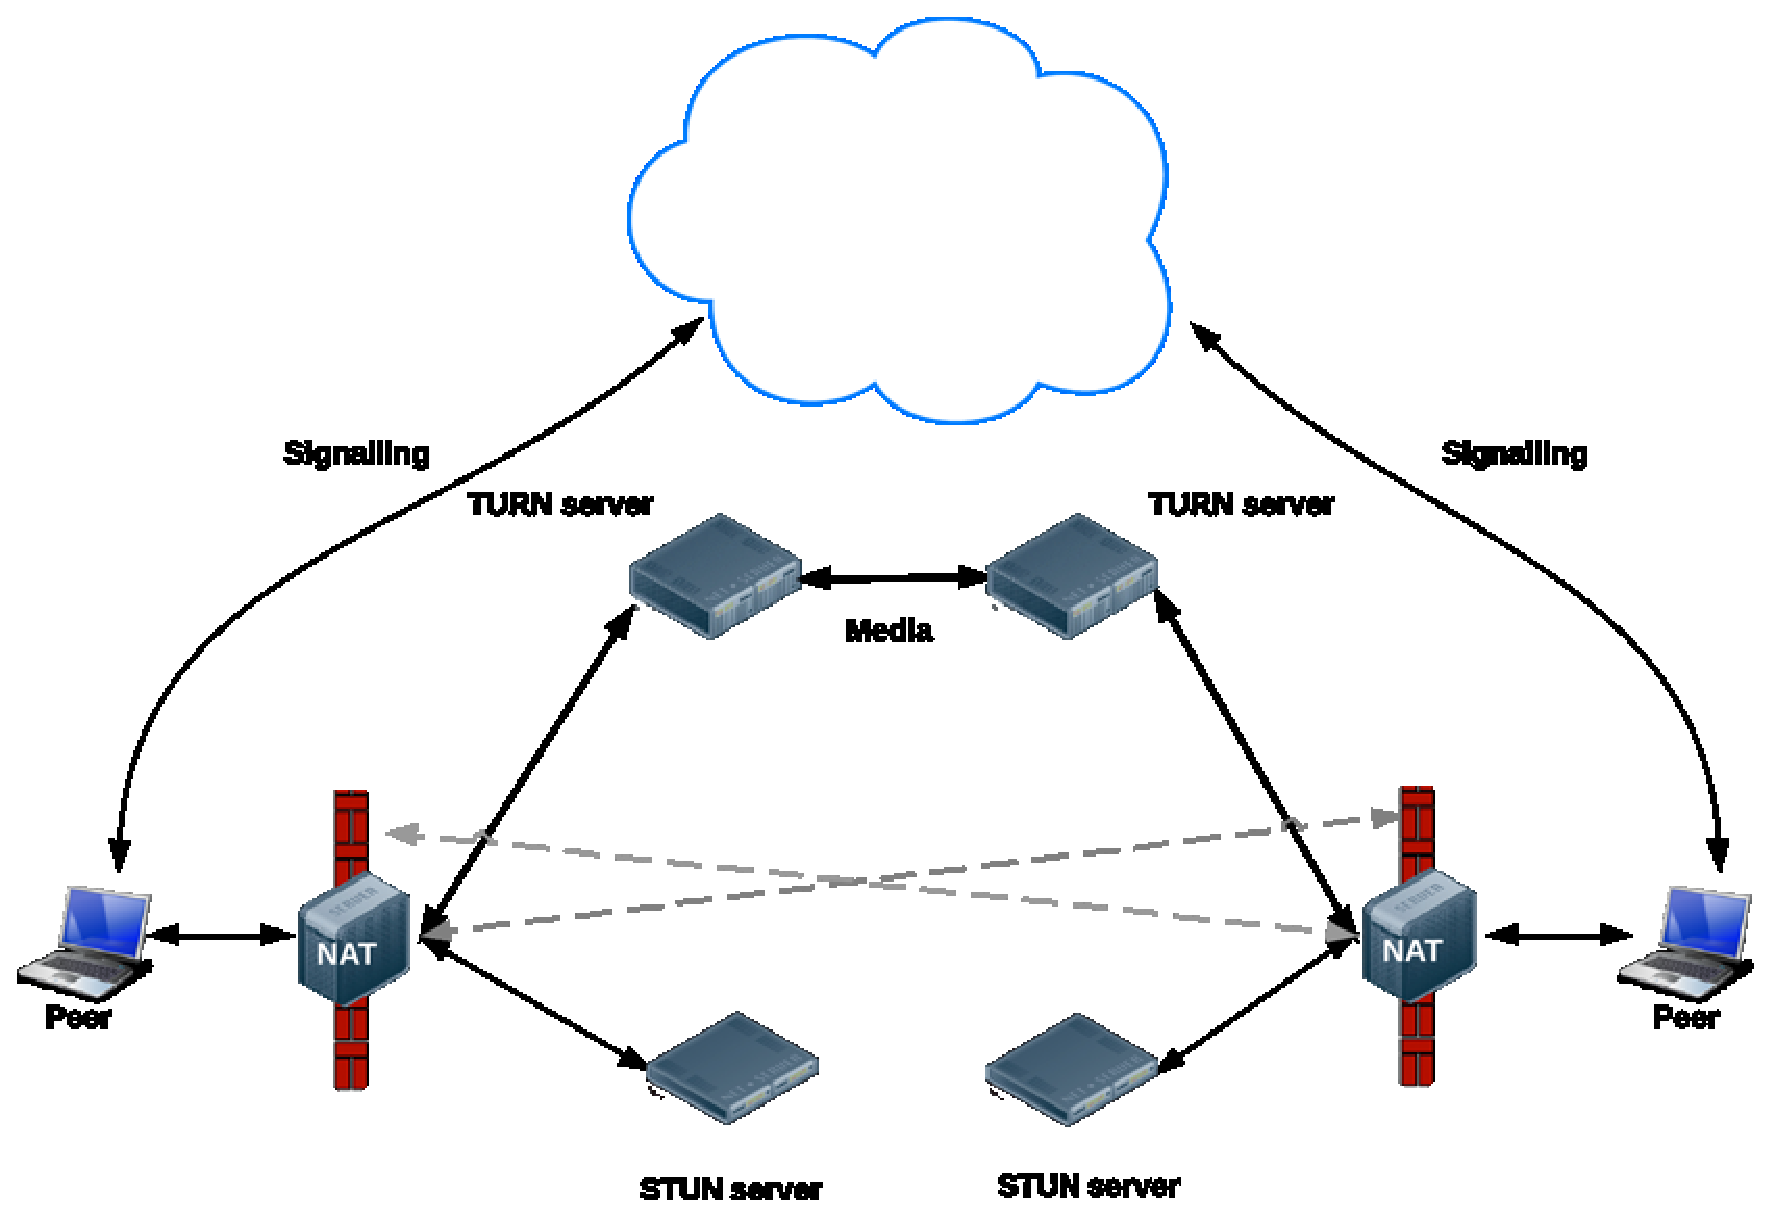
\includegraphics[width=0.7\columnwidth]{turn.eps}
	\caption{STUN, TURN et signalisation}
	\label{fig:turn}
\end{figure} 

La Figure \ref{fig:turn} représente le cas le plus complexe que l'on peut 
rencontrer pour établir une connexion WebRTC. Le plus simple des réseaux P2P 
peut être résumé comme deux machines connectées directement l'une à l'autre. 
Cette vision un peu utopique ne tient pas compte des routeurs qu'une connexion 
internet peut rencontrer. 
Chaque routeur peut posséder un \gls{NAT} afin de faire correspondre 
les adresse IP à d'autres adresse IP (dans le cas d'un intranet par exemple). 
Cela permet de faire communiquer des machines non uniques et non routables en 
faisant semblant d'utiliser des adresses externes, uniques et routables. 
Pour permettre à un client situé derrière un routeur \gls{NAT} de connaître son 
adresse IP publique et le type de serveur \gls{NAT}, l'utilisation d'un serveur 
\gls{STUN} est requise. 
L'utilisation d'un \gls{NAT} dynamique impose des restrictions sur l'adresse de  
destination. Dans ce cas, le \gls{STUN} est remplacé par l'utilisation d'un serveur 
\gls{TURN}. Le \gls{TURN} est considéré comme une extension du \gls{STUN} et fait office de 
proxy. 
Une fois que le client est parvenu à récupérer une adresse IP, il peut participer à 
l'initialisation d'une connexion WebRTC (signalisation). L'utilisation de protocoles 
tels que \gls{ICE} avec son \gls{ICEF} permet de faciliter la mise en relation des 
clients derrière un \gls{NAT}. Le \gls{ICEF} choisit le chemin le plus court entre les 
deux pairs et va utiliser le protocole adapté pour établir la connexion (\gls{STUN} 
d'abord puis en cas d'échec, \gls{TURN}).


%Du point de vue sécurité des communications, le standard requiert 
%obligatoirement le chiffrement pour tous les composants \gls{WebRTC}. 
%Cependant, les mécanismes de signalisation n'étant pas définis par le standard, 
%cela signifie que les développeurs sont assez libres d'utiliser les protocoles de 
%signalisation qu'ils souhaitent (SIP, \gls{WebSocket}, \gls{XHR}, une \gls{API} 
%externe\dots). Dans le cas où la connexion subit une attaque, la connexion peut 
%être stoppée, 
%redirigée ou enregistrée, altérée ou encore subir de l'injection de contenu. Pour 
%sécuriser la connexion l'utilisation de protocoles sécurisés comme HTTPS ou 
%\gls{WebSocket} (basé sur \gls{TLS}), assure qu'un message ne peut être 
%déchiffré.

\subsection{Quel protocole dans quel EVC3D ?}
%\improve{reformuler paragraphe}
Un des aspects prépondérant dans les \gls{EVC3D} concerne la communication et 
la transmission des données lors de la collaboration. Que ce soit dans dans un 
\gls{EV}, un jeu sérieux multi-utilisateur, les 
participants interagissent en (quasi) temps réel alors qu'ils sont situés à 
différents endroits géographiques. 
Le développement d'un \gls{EVC3D} nécessite donc des connaissances issues de 
plusieurs domaines comme la conception et l'implémentation de protocoles 
réseaux et de réseaux distribués.

Comme l'indique \cite{Roberto2014}, le protocole le plus souvent rencontré dans 
les \gls{EVC3D} est l'\gls{UDP}. 
Cette prépondérance s'explique selon deux facteurs. Premièrement, dans des 
réseaux où l'accès est fiable, ces environnements n'ont 
pas (ou peu) de perte de paquet (ex : \gls{LAN}). Deuxièmement, dans un contexte 
d'application où la perte de paquet n'est pas critique (ex : jeu vidéo, diffusion en 
continu de son, vidéo, \gls{3D}\dots). 
\gls{UDP} peut également s'utiliser dans tout type de réseaux -- \gls{LAN} ou 
\gls{WAN} (comme internet) --, car il est basé sur des datagrammes. Le fait qu'il 
n'effectue pas de vérification de délivrance lui donne un avantage quant 
à la taille des données gérées dans les \glspl{EVC}. La responsabilité de 
vérifier quels sont les 
paquets qui n'ont pas été délivrés et leur ordre d'arrivée incombe à l'application.

\gls{TCP} est le protocole qui vient en seconde position. Les \gls{EVC3D} qui sont 
implémentés sur des réseaux haut-débit ne sont pas affectés par les étapes de 
vérifications que nécessitent une connexion \gls{TCP}. D'après \cite{Sung2006}, 
l'utilisation du protocole \gls{TCP} sur internet dans le cadre des \gls{EVC3D} n'est 
pas recommandée à cause de la taille de l'en-tête et du ACK qui réduisent le débit 
des paquets.
Dans ce contexte, le protocole \gls{UDP} obtient de meilleurs résultats dans le cas 
où le flux de données est local (\gls{LAN}). 
Les protocoles les plus adaptés pour communiquer dans un \gls{EVC3D} sont 
cependant \acrshort{SCTP} et \gls{RTP}/\gls{RTCP}. Ils combinent les 
fonctionnalités de 
\gls{TCP} et \gls{UDP} et sont optimisés pour les applications multimédia (flux et 
temps-réel). \gls{SCTP} offre la possibilité de choisir entre un système de 
livraison fiable (pour les paquets clés par exemple) ou non fiable (pour des mises 
à jour normales).

Depuis plusieurs décennies, les architectures \gls{P2P} sont utilisées dans les 
\gls{EVC}. Par exemple, l'assistance au rendu \gls{3D} par les pairs \cite{Zhu2011}
est une méthode qui permet aux pairs hébergés sur des appareils avec des capacités 
limitées (bande passante, processeur, processeur graphique) de demander une 
partie du contenu de l'environnement aux autres pairs.
Ce système d'assistance par les pairs peut également être utilisé pour améliorer le 
rendu dans les environnements virtuels en ajustant la qualité du rendu en fonction 
du coût de calcul. 
Des systèmes récents comme celui de Martinez et al. \cite{Martinez2009} 
utilisent la localisation d'un utilisateur pour transmettre uniquement les mises 
à jours à son plus proche voisin.  
Koskela et al. \cite{Koskela2014} sont allés plus loin dans cette direction en 
proposant la méthode RADE (\textit{Ressource-Aware P2P-assisted 3D Delivery 
Method}). RADE repose sur l'utilisation du \gls{P2P} pour alléger le chargement 
et donc réduire le coût d'exploitation des fournisseurs de service. Les 
clients peuvent également être inclus en tant que fournisseurs de services dans 
cette architecture. 
Le système utilise un serveur qui connaît la localisation des ressources et 
effectue le \textit{load balancing} nécessaire pour distribuer les données en 
fonction des capacités des clients. L'impact énergétique d'un tel système a été 
évalué sur les mobiles ciblant trois optimisations possibles : la qualité visuelle, les 
performances et la consommation d'énergie. 
Les architectures hybrides, combinant client-serveur et \gls{P2P} sont également 
des solutions utilisées dans le cadre de l'apprentissage en ligne 
\cite{Ekadiyanto2012} et du BIM \cite{Chen2014} par exemple. 
En général, les systèmes \gls{P2P} semblent n'être supportés que dans les 
environnements virtuels \gls{3D}. Ce phénomène est probablement dû au lien étroit 
entre la séparation spatiale de l'utilisateur et le besoin de distribuer les données à 
tous les participants.
%
%
%	\subsection{Introduction}
%	\subsection{Les approches centralisées}
%	\subsection{Les approches décentralisées}
%	\subsection{Conclusion}

%\section{Systèmes d'édition collaborative}
%	\subsection{Le modèle de cohérence CCI}
%	\subsection{Les approches pour les données 3D}
%	\subsection{Conclusion}

\section{Les systèmes distribués orientés événements pour la collaboration}

	\subsection{Introduction}
% old evenements et collaboration
Les systèmes orientés événements (\gls{EDA}) sont très populaires lorsqu'il s'agit 
de systèmes collaboratifs \cite{Helmer2011}. Les événements sont utilisés dans la 
communauté  \gls{CSCW} pour la sensibilisation aux activités distribuées 
\cite{Cai2014a} et également l'analyse de conceptions collaboratives 
\cite{Bang2017}, la spécification d'événements composites pour le support de la 
collaboration dans la conception logicielle \cite{Yuan2002} ou encore la définition 
de patrons de conception dédiés à la collaboration dans les architectures basées 
événements \cite{Verginadis2009}. Dans ce dernier domaine 
Papageorgiou et al. \cite{Papageorgiou2011} proposent un assistant à la 
création de ces patrons dédiés à la collaboration. Ils s'appuient sur un système de 
recommandation basé sur le contexte qui utilise une représentation sémantique 
(\gls{OWL}).

CoDesign est un exemple de \gls{framework} permettant de faire de la 
conception logicielle de manière collaborative \cite{Bang2010}. L'utilisation d'une 
architecture basée événement permet à l'application d'être très extensible car très 
peu couplée. Chaque instance CoDesign intègre un intergiciel appelé CoWare en 
charge de la synchronisation de contenus édités de manière concurrente sur les 
différentes instances CoDesign, ainsi qu'un module chargé de notifier les 
architectes de situations de modélisation conflictuelles. 


Eventuate est une plateforme qui se base sur un modèle de programmation 
événementielle ayant pour but de résoudre les problèmes liés à la gestion de 
données distribuées inhérents aux architectures microservices en utilisant \gls{ES} et
\gls{CQRS}. Une de leurs applications exemples est un tableau Kanban collaboratif 
temps réel construit sur leur plateforme
\footnote{https://github.com/eventuate-examples/es-kanban-board}. 
%	\subsection{Les événements comme base du comportement réactif}
	\subsection{Systèmes Publish-Subscribe}

Le système \glsreset{PubSub}\gls{PubSub} est un mécanisme basé sur le 
paradigme des 
messages qui est beaucoup utilisé en \gls{EP}. 
Les éditeurs (ceux qui émettent des messages) et les abonnés 
(ceux qui souscrivent) sont couplés de manière lâche. 
Autrement dit, l'éditeur n'est pas forcément au courant de l'existence de 
ses abonnés et n'a donc pas de contrainte forte le liant à ces derniers. 
De son côté, l'abonné est souvent indifférent à l'éditeur qui lui 
fournit les événements qui l'intéressent. La Figure \ref{fig:pubsub} représente le 
modèle \gls{PubSub}.
Le service de notification d'événement est utilisé comme passe-plat d'événements 
entre l'éditeur et les abonnées. Son rôle est de gérer les abonnements 
(abonnement / désabonnement) et de notifier les abonnés concernés par la 
publication d'un événement par un éditeur.
%TODO expliquer la figure 

\begin{figure}[ht!]
	\centering
	\inputTikZ{1}{eps/tikz/pubsub}
	\caption{Architecture Publish-Subscribe}
	\label{fig:pubsub}
\end{figure}


Les modèles utilisant le paradigme \gls{PubSub} supportent naturellement une 
communication plusieurs-à-plusieurs (\textit{many-to-many}) 
entre les éditeurs (\textit{publishers}) et les abonnés (\textit{subscribers}).  
De cette manière, le passage à l'échelle d'une application est facilité 
grâce à une topologie du réseau plus flexible. 


Pour répondre à des besoins de passage à l'échelle, d'interopérabilité, de fiabilité, 
d'expressivité et d'utilisabilité, un modèle \gls{PubSub} peut s'appuyer sur :
\begin{itemize}
\item
 le contenu du message transmis (content-based)  -- l'intérêt de l'abonné est décrit par le type et les valeurs de l'événement qu'il veut recevoir ;
\item le sujet du message (topic-based) -- le système dédie un canal à des événements d'un type en particulier. Les éditeurs publient sur le canal approprié, alors que les abonnés exprime leur intérêt à recevoir les messages d'un certain type.  
\end{itemize}
En spécifiant d'abord le type et ensuite en filtrant sur les attributs des 
événements, ce modèle rend le routage des données intuitif pour le 
développement d'applications distribuées à grande échelle comme le commerce 
en ligne (\textit{e-commerce}). Scribe \cite{Castro2002} et Hermes 
\cite{Pietzuch2002} sont des exemples de systèmes \gls{PubSub} basés sur les 
\glspl{DHT}. 
Le premier se concentre sur la catégorie du sujet (\textit{topic-based}) tandis que 
le second supporte à la fois la communication orientée sujet et la communication 
orientée contenu (\textit{content-based}) en utilisant un 
filtrage par agrégat. Les deux utilisent un n\oe ud \textit{rendezvous} pour chaque 
sujet ou type d'événement dans la couche réseau et construisent et maintiennent la 
distribution à partir de ce n\oe ud \textit{rendezvous}. TERA \cite{Baldoni2007} 
propose une dissémination sur deux couches orientées sujets. Le but est d'effectuer 
une distribution uniforme en fonction des intérêts des n\oe uds. La dissémination 
se déroule en deux phases. Pendant la première phase, un algorithme de marche aléatoire (succession de pas aléatoires dans le graphe)
est utilisé sur la couche basse qui connecte les n\oe uds dans le but de localiser 
le n\oe ud qui a souscrit au sujet. La seconde phase commence lorsqu'un 
\textit{subscriber} est trouvé pour le connecter à la grappe (\textit{cluster}) correspondante au 
sujet  sur la couche haute. C'est là que l'événement est disséminé.

En juin 2017, Leonardo Quernozy présente une rétrospective des systèmes 
\gls{PubSub} en \gls{P2P} massifs lors de la conférence DEBS'2017 à 
Barcelone. 
Les premières traces d'une telle architecture remontent à 1987 avec 
la publication de Birman et Joseph \cite{Birman1987} lorsqu'ils évoquent \og 
the ''News'' service in the ISIS system\fg{}:

\blockcquote{Birman1987}{
	\og\textit{ This service allows processes to enroll in a 
		system-wide news facility. Each subscriber receives a
		copy of any messages having a "subject" for which it 
		has enrolled in the order they were posted. Although 
		modeled after net-news, the news service is an active 
		entity that informs processes immediately on learning 
		of an event about which they have expressed interest.}\fg{}
}

Après cette publication, les premiers systèmes \gls{PubSub} commencent à 
se développer. Le concept de routeur d'information est introduit par Oki et al. 
\cite{Oki1993} : un seul bus d'information pour tous les services, objets, 
données\dots Les protocoles de communication ont une sémantique minimale, 
les objets (instances de classe) sont auto-descriptifs - i.e. ils sont 
capables d'introspection (service, opérations, attributs) pour adapter leur 
comportement au changement, les types peuvent être définis dynamiquement et 
la communication est anonyme. 
Puis des solutions plus avancées sont apparues avec le projet 
GRYPHON d'IBM \cite{Banavar1999}, SIENA \cite{Carzaniga2000}, REBECA 
\cite{Parzyjegla2010} et également REDS, JEDI, PADRES présentés plus en 
détails dans \cite{Tarkoma2012}.
Ces différentes solutions ont été conçues comme des systèmes de gestion avec 
des gestionnaires d'événements dédiées. Le passage à l'échelle est 
principalement effectué par un routage efficace des événements (comme le 
filtrage d'événements). Seuls quelques travaux ont utilisé le concept de grappe  
par intérêt (\textit{clustering}) comme moyen de réduire le nombre de 
notifications d'événement et éviter la surcharge. 
A partir des années 2000, les systèmes \gls{P2P} ont commencé à émerger avec 
l'apparition de Gnutella\cite{Ripeanu} et consorts, les \glspl{DHT} (Chord, Pastry, 
Kademlia) et  réseaux non-structurés (Cyclon, Scamp, ADH). 
Ces systèmes ont pour objectif de gérer des réseaux massifs, dynamiques 
(client gagnés / clients perdus), résistants aux erreurs, et offrants des primitives 
de communications basiques.
Les réseaux \gls{P2P} promettent alors des propriétés intéressantes pour les 
infrastructures logicielles comme les systèmes \gls{PubSub} concernant le 
passage à l'échelle. Cependant, les systèmes \gls{PubSub} d'alors reposent sur 
une connaissance 
totale du réseau pour être efficaces, du fait de leur taille limitée. À grande échelle, 
suivre et collecter l'information de chacun devient complexe. 
Le modèle \gls{PubSub}, très peu couplé est une approche efficace pour collecter et analyser 
les échanges dans les réseaux \gls{P2P}. La paternité de chaque événement peut être 
tracée facilement tout au long du routage notamment dans un environnement décentralisé.
Il est cependant important de garder en tête que la connaissance peut vite devenir 
viciée (\textit{staleness}) dans un système dynamique décentralisé, ce qui impose de trouver une méthode 
efficace pour garantir la fraîcheur des données, leur accessibilité avec une gestion 
de la dynamicité des pairs efficace.

Les systèmes \gls{PubSub} ont donc l'avantage de proposer une \gls{EDA} dont le 
fonctionnement s'adapte à plusieurs types de communication, que ce soit client-serveur
ou P2P. Cette flexibilité a l'avantage de proposer un système à couplage 
lâche qu'il reste cependant difficile d'observer à grande échelle.

\subsubsection{Outils de surveillance, contrôle de performances et validation ergonomique}
Dans un système distribué comme \gls{PubSub}, les outils de comparaison 
sont souvent très hétérogènes et ne permettent pas forcément d'évaluer sur une 
même base la montée en charge. 
Carzaniga and Wolf \cite{Carzaniga2002} proposent quelques 
lignes directrices pour concevoir une suite de \textit{benchmark} dans un système 
\gls{PubSub}, sans fournir de résultat spécifique, dont le but est double : la 
validation de l'interface et l'évaluation de la performance. 
La pertinence de l'interface a été définie par une série de questions / réponses 
posée au développeur. Elle adresse plusieurs aspects propres à l'\gls{IU} : 
\begin{itemize}
	\item le modèle de publication (structure, domaines de valeur, taille des objets);
	\item le modèle de souscription (portée de l'évaluation d'une publication reçue, 
	type de langage, expressivité du langage pour la sélection);
	\item les méthodes d'accès à l'interface (accès local, mémoire partagée) ; 
	\item la portabilité du système (support multi-plateforme) ;
	\item le type de service (fiabilité) et les fonctionnalités auxiliaires. 
\end{itemize}

Pour évaluer la charge de travail d'un système distribué basé événements, 
Kounev et al. \cite{Kounev2008} ont utilisé des techniques d'analyse 
opérationnelle pour caractériser le trafic du système et dériver une approximation 
de la moyenne des délais de livraison d'événements. 

%TODO precisier quelles recherches
Beaucoup de recherches ont été menées dans le but d'améliorer les performance 
des systèmes collaboratifs utilisant une architecture distribuée. Bien que ces 
approches permettent de passer à l'échelle de grandes quantités de données, cela 
requiert de lourds investissements pour installer et maintenir plusieurs serveurs 
dédiés. Une alternative à bas coût est d'utiliser les différents clients à disposition 
(qui sont en relation par le biais de la collaboration) pour avoir un traitement réparti 
des données sur les utilisateurs (\textit{crowd computing})\cite{Li2015}. De ce fait, le 
contenu \gls{3D} est distribué par les pairs et non plus par le serveur. En 
combinant les 
ressources réseau du serveur et de plusieurs clients, on peut réaliser une 
distribution des données (événements) en améliorant les performances du 
système pendant les sessions de travail collaboratif. 




\subsection{Domain Driven Design}
%\subsection{Domain Driven Design : lier le fonctionnel et le code}
	
\glsreset{DDD}\gls{DDD} ou Conception Pilotée par le Domaine est une 
approche de 
développement logicielle qui a pour objectif de définir une vision et un langage 
partagé (\textit{ubiquitous language}) pour les personnes impliquées dans la 
construction d'une application \cite{Evans2003}.
Avec le \gls{DDD}, un projet est vu à travers le prisme du domaine d'application 
qui le concerne (métier) et la logique du domaine en basant des conceptions complexes
sur un modèle du domaine. Cela s'inscrit dans l'objectif d'initier une collaboration 
créative entre les experts techniques et les experts du domaine pour produire un modèle 
conceptuel -- qui relève de problèmes spécifiques au domaine -- raffiné itérativement.
Les différents concepts du \gls{DDD} sont listés en suivant :
\begin{itemize}
	\item \textit{Le contexte.} est le cadre dans lequel un mot apparaît qui détermine sa 
	signification ;
	\item \textit{Le domaine.} est une ontologie, une influence, ou une activité. 
	L'étendue du sujet auquel l'utilisateur applique un programme est le domaine 
	du logiciel ;
	\item \textit{Le modèle.} est un système d'abstractions qui décrit les aspects 
	sélectionnés du domaine et qui sont utilisés pour résoudre les problèmes liés 
	à ce domaine ;
	\item \textit{Le langage partagé.} est un langage structuré autour du modèle du 
	domaine utilisé par tous les membres de l'équipe pour faire référence aux 
	activités de l'équipe permettant d'éviter la redondance et les ambigüités dans
	un contexte donné.
\end{itemize}

\begin{figure}
	\noindent
	\centering
	\includegraphics[width=0.9\columnwidth]{ddd.eps}
	\caption[Illustration du patron \gls{DDD} et de ses artefacts]{Illustration du 
	patron \gls{DDD} et de ses artefacts (issue de 
	\cite{Avram2006} sous licence Creative Commons)}
\label{fig:ddd}
\end{figure}

Le \gls{DDD} permet de connecter le modèle et son implémentation en offrant 
plusieurs avantages. La plasticité du système est mise en avant par l'expression 
de règles et de comportements qui facilitent les changements fréquents.
L'accent mis sur l'identification des interactions dans le système encourage la 
mise en \oe{}uvre d'une interface orientée tâches (\textit{task-based UI}).
La testabilité fonctionnelle est intégrée via les règles métier explicitées 
et concentrées dans une couche spécifique de l'application. Cela les rend 
plus facilement identifiables et testables automatiquement.
La robustesse est améliorée face aux changements dans le système d'information.

En \gls{DDD}, il existe des artéfacts qui permettent d'exprimer, créer et stocker un 
modèle lié à un domaine (voir Figure \ref{fig:ddd}). Parmi les principaux se trouvent 
:
\begin{itemize}
	\item L'\textbf{entité} (\textit{entity}) : un objet qui n'est pas défini par ses 
	attributs mais plutôt par une continuité et son identité. 
	Par exemple, chaque scène possède des maillages qui utilisent des 
	géométries. Si l'on considère un maillage comme unique dans chacune des scènes alors chaque 
	maillage est une entité. Si on considère que ce sont les mêmes maillages qui 
	sont réutilisés alors un maillage est considéré comme un objet-valeur.
	
	\item L'\textbf{objet-valeur} (\textit{value object}) : un objet qui contient des 
	attributs mais n'a pas d'identité conceptuelle. Il doit être traité comme un objet
	immuable. Par rapport à l'exemple précédent, on peut considérer que si les 
	géométries sont réutilisées d'une scène à l'autre, ce sont des objets-valeurs qui 
	ne seront jamais modifiés car les utilisateurs ne sont intéressés que par les 
	informations qu'elles portent.
	
	\item L'\textbf{agrégat} (\textit{aggregate}) : une collection d'objets qui sont 
	liés ensemble par une entité commune (\textit{root entity}), connue sous le nom 
	d'agrégat souche (\textit{aggregate root}). Ce dernier garantit la cohérence des 
	modifications faites au sein de l'agrégat en interdisant aux objets externes de 
	faire référence à ses membres. Par exemple, dans une modélisation \gls{3D} 
	collaborative un utilisateur ne peut pas modifier le nom d'un autre utilisateur. Un 
	maillage n'a également pas d'intéret à connaître les informations des 
	utilisateurs, c'est la scène qui gère l'interface entre les maillages et les 
	utilisateurs.
	\item L'\textbf{événement du domaine} (\textit{domain event}) : un 
	événement auquel 
	l'expert du domaine s'intéresse. Il est défini par un objet du domaine.
	\item Le \textbf{dépôt} (\textit{repository}) : les méthodes pour récupérer les 
	objets du domaine doivent être déléguées à un \textbf{dépôt} spécialisé afin de 
	faciliter les implantations 
	alternatives de stockage.
\end{itemize}



Les notions plus détaillées qui se rapportent au \gls{DDD} sont présentées dans 
\cite{Evans2003} et \cite{Vernon2013}\footnote{Les différents ouvrages publiés par 
Vernon s'attachent également à montrer la nécessité pour les différentes 
branches de l'informatique à proposer des 
systèmes d'information plus robustes et flexibles face aux nouvelles demandes.}.
%\info{source: 
%http://blog.octo.com/domain-driven-design-des-armes-pour-affronter-la-complexite/}

Le \gls{DDD} a également l'avantage de fonctionner en harmonie avec les 
principes de l'\gls{ES}. L'approche logicielle \gls{DDD} étant conçue pour refléter 
les événements se déroulant dans la réalité métier qui ne sont pas 
interchangeables -- la plupart du temps. L'utilisation d'architectures 
basées événements est naturelle dans ce genre d'environnement. 

Les disciplines liées à la \gls{3D} dans un contexte industriel ont besoin de pouvoir 
communiquer sur un langage partagé pour permettre à chacun des 
intervenants de s'exprimer dans la création du produit. Par exemple, la \gls{CAO} 
est très utile dans un contexte d'ingénierie grâce à l'utilisation de quatre propriétés 
fondamentales telles que l'historique, les fonctionnalités, la paramétrisation et le 
haut niveau de contrainte.



\subsection{Command Query Responsability Segregation}
%	\subsection{Command Query Responsability Segregation : garantir de 
%	l'intégrité 
%	des données }
\label{sec:CQRS}
Une solution architecturale courante en \gls{DDD} contient quatre 
couches : l'interface utilisateur (présentation), la couche application (coordination 
de l'activité de l'application), la couche domaine (c\oe ur du logiciel métier), la 
couche infrastructure (interface entre les couches, persistance des objets 
métier\dots). La Figure \ref{fig:dddcqrs} montre que ces quatre couches s'accordent
bien avec l'architecture \gls{CQRS} qui sépare les flux d'écriture et de lecture dans 
le logiciel.

Introduit par Greg Young en 2009 \cite{Young2009}, \gls{CQRS} est un patron de 
conception qui repose sur le principe de séparation des composants de traitement 
métier de l'information (écriture) et de la restitution de l'information (lecture). Le 
cadre offert par ce principe permet de lever certaines contraintes d'architecture 
comme le passage à l'échelle en faisant apparaître de nouvelles forces : la gestion 
de la concurrence dans la collaboration sur des règles métiers propres à la 
modélisation \gls{3D} dans des cadres d'application spécifiques. En effet, selon le 
type d'application, un ensemble de règles régit les droits concernant les types de 
modifications acceptables et qui est autorisé à le faire.

\begin{figure}[ht]
	\noindent
	\centering
	\inputTikZ{1}{eps/tikz/ddd/dddcqrs}
	\caption{Architecture en 4 couches du DDD (gauche) en miroir avec 
		l'architecture CQRS 
		(droite)}
	\label{fig:dddcqrs}
\end{figure}


Le caractère vicié d'une donnée dans un environnement 
collaboratif est récurrent. Une fois que la donnée a été montrée à un utilisateur, la 
même donnée peut être changée par un autre utilisateur, elle est altérée. 
\gls{CQRS} pallie cela en répondant aux besoins suivants :
\begin{itemize}
	\item \textbf{En traitement / écriture} : besoins transactionnels, garantie de cohérence 
	des données, de normalisation ;
	\item \textbf{En consultation / lecture}: dénormalisation, passage à l'échelle.
\end{itemize}

La plupart des architectures en couches ne font pas explicitement référence à ces 
problèmes. Le fait de tout sauvegarder dans une base de données centralisée peut 
être une étape dans la gestion de la collaboration, mais l'altération des données est 
souvent exacerbée par l'utilisation de caches comme accélérateur de performance.
L'immuabilité en \gls{CQRS} est un concept clé qui prévient la  
modification de l'état interne d'une commande ou d'un événement. Les 
commandes sont immuables car leur usage nécessite un envoi direct au domaine 
pour être traitées. Quant aux événements, ils sont immuables car ils représentent 
ce qui s'est produit dans le passé (qu'on ne peut donc pas changer). 

\subsection{Event Sourcing}
%\subsection{Event Sourcing : certifier la fiabilité et traçabilité des données}
\label{sec:es}

Le Reactive Manifesto, apparu en 2014, est un document qui résume les 
propriétés clés des systèmes distribués et encourage notamment le 
développement de systèmes \og plus flexibles, à couplage faible et 
extensibles\fg{}\cite{Boner2014} comme le \gls{CQRS} et l'\gls{ES}.

L'\glsreset{ES}\gls{ES} est une approche complémentaire au \gls{CQRS} pour 
gérer la concurrence des données et capturer l'intention de l'utilisateur. 
Ce patron de conception stocke les événements en mode ajout seulement 
(\textit{append-only}) pour sauvegarder le résultat des commandes sur le 
domaine. Cela permet de conserver tous les changements qui ont mené à un 
état plutôt qu'uniquement l'état actuel. Ce paradigme permet de recréer n'importe quel 
état d'un agrégat à partir d'une séquence d'événements donnée. Cette séquence 
représente la source primaire de données du système, i.e. elle immuable et 
toujours accessible dans le système. 
L'\gls{ES} réduit l'essentiel de l'information à l'événement permettant de passer d'un 
état à l'autre. L'événement est générique et auto-descriptif ce qui permet réduire la 
complexité des structures de données en encapsulant de la connaissance dans un élément 
atomique. 

L'\gls{ES} est souvent présent dans des architecture asynchrones qui ont 
l'avantage de pouvoir utiliser des queues de message, plusieurs bases de 
données, et où la partie lecture est éventuellement consistante.
La plupart de la littérature concernant ce patron se trouve en ligne, dans des 
billets de blog, des présentations ou de la documentation logicielle. La 
littérature académique est relativement réduite et se rapporte principalement
à l'étude de l'évolution de graphes dans le temps \cite{Erb2015,Erb2017}. Cette section fournit un aperçu des différentes 
définitions données de l'\gls{ES} et du vocabulaire lié à ce patron de conception.

Martin Fowler a été le premier à utiliser le terme d'\acrlong{ES} en 2005\cite{Fowler2005}. 
Il définit l'\gls{ES} comme \og une série de changements de l'état d'une 
application\fg{}. Il voit les événements comme immuables et le journal 
d'événement (\textit{event log}) comme un stockage linéaire 
(\textit{append only store}) des événements (Figure \ref{fig:es-event}). 
Les événements ne sont jamais supprimés, le seul moyen de l'\og annuler\fg{} consiste à 
générer un événement rétroactif. 
Une fois qu'un événement rétroactif est ajouté, l'événement rétroactif agit à 
l'inverse de l'événement précédent pour compenser ses effets 
(Figure \ref{fig:es-transaction-delete}). 
Dans ce billet, Fowler n'établit pas clairement la distinction entre les 
événements et les commandes qui déclenchent ces événements. Ce problème est 
considéré dans plusieurs travaux fondamentaux \cite{Prakash1994,Sun2002,Weiss2009a,Weiss2010}, 
et approfondi par une revue de Chen et al. \cite{Cheng2013}.

Greg Young, important contributeur au domaine de l'\gls{ES} (et particulièrement du \gls{CQRS}), 
décrit l'\gls{ES} comme \og le stockage de l'état courant sous la forme 
d'une série d'événements et la reconstruction de l'état du système en rejouant 
cette série d'événements\fg{}. D'après lui, le journal d'événements a également 
un comportement linéaire : les événements qui sont déjà arrivés ne peuvent 
être défaits. Ce que Fowler appelle événements rétroactifs, Young le décrit 
comme des actions inverses.

Udi Dahan est également un auteur de billets de blog 
prolifique sur les systèmes \gls{ES}. Dans sa définition de l'\gls{ES}, Dahan 
insiste sur le fait que \og l'état du modèle du domain est persisté comme un 
\textit{flux} d'événements plutôt qu'un simple instantané\fg{}.


%
	\begin{figure}[!h]
		
		\centering
		\noindent
		\subfloat[Nouvel événement en \gls{ES}]{
			\inputTikZ{1}{eps/tikz/eventsourcing/es.tex}
			\label{fig:es-event}
		}
	
	\subfloat[Transaction avec compensation en \gls{ES}]{
		\inputTikZ{1}{eps/tikz/eventsourcing/escompensation.tex}
		\label{fig:es-transaction-delete}
	}
		\caption{Transaction en \gls{ES}}
		\label{fig:es-transaction}
	\end{figure}

	
	\begin{figure}[t]
		\centering
				\subfloat[Lecture normale d'un agrégat]{
			\includegraphics[width=0.5\textwidth]{eps/tikz/streams/aggregate-normal.pdf}
			\label{fig:es-without-snapshot-aggregate}
		}
		
		\subfloat[Reconstruction sans la notion de Snapshot]{
			\includegraphics[width=0.45\textwidth]{eps/tikz/streams/snapshot-no.pdf}
			\label{fig:es-without-snapshot}
		}\hfill
		\subfloat[Reconstruction avec la notion de Snapshot]{
			\includegraphics[width=0.45\textwidth]{eps/tikz/streams/snapshot-yes.pdf}
			\label{fig:es-snapshot}
		}
		\caption{Snapshot en \gls{ES}}
	\end{figure}

Les avantages et les inconvénients de l'approche \gls{ES} dépendent du
cadre dans lequel elle est utilisée. En reprenant ceux cités par Klamer 
\cite{Klamer2013a}, ils peuvent être envisagés sous l'angle de la modélisation 
\gls{3D} 
collaborative.

L'\gls{ES} peut apporter beaucoup d'avantages à une application, notamment 
lorsque les besoins en traçabilité de l'information sont importants comme dans 
la modélisation collaborative de données \gls{3D}.
L'historique du système est accessible tout au long de la vie de l'application, ce 
qui implique qu'il est non seulement possible d'accéder à l'état courant du 
système, mais également à toutes les actions ayant mené jusqu'à cet état. C'est 
un avantage certain pour les système critiques, les applications d'Informatique 
Décisionnelle ou les applications collaboratives. La pratique la plus 
courante est de proposer un système principal et d'ajouter une multitude de 
sous-systèmes qui enregistrent les différentes métriques (analyse d'un ou 
plusieurs axes, \textit{reporting} sur une propriété) du système principal. Avec 
l'\gls{ES}, il est toujours possible de regarder \og dans le passé\fg{} et de 
récupérer les données à partir de ce moment. Par comparaison, les avantages 
exprimé par Fowler \cite{Fowler2003} de l'\gls{ES} sur l'Active Record sont :
\begin{itemize}
	\item un journal complet de tous les changements d'état,
	\item une traçabilité et un débogage efficace,
	\item de très bonnes performances,
	\item pas de mapping objet-relationnel (ORM).
\end{itemize}

	
\paragraph{Exemple} 
Une revue de projet d'une scène est effectuée dans le cadre d'une application 
collaborative de modélisation \gls{3D} en ligne. Le chef de projet remarque qu'un 
objet a subi énormément de modifications par rapport aux autres. Il examine en 
particulier cet objet pour en connaître les causes. Voici deux exemples 
d'observations possibles : 
\begin{enumerate*}[label=(\roman*)]
	\item les spécifications ne sont pas assez claires ;
	\item deux collaborateurs sont opposés sur la façon de modifier l'objet.
\end{enumerate*}
L'origine de ces changements identifiée, le chef de projet pourra alors intervenir 
et clarifier le sujet. 

\paragraph{Résolution} Avec un système classique, la fonctionnalité doit être 
créée pour enregistrer ce traitement, puis être testée et implémentée (dans cet 
exemple, il en faudrait deux). Ensuite seulement, un rapport pourra être délivré. 
Dans un environnement utilisant l'\gls{ES}, tous les événements existent déjà 
donc les données sont déjà disponibles et ont seulement à être analysées 
(dans notre exemple, les informations sont inhérentes aux événements). De plus, 
les événements étant stockés depuis le début de la vie -- mise en route -- de l'application , beaucoup plus de données peuvent être analysées. Par 
exemple : demander toutes les modifications d'un objet depuis la dernière 
connexion d'un utilisateur pour lui communiquer visuellement les différences par 
rapport à sa dernière visite.



En revanche, les performances de l'application peuvent être affectées par 
l'utilisation de 
l'\gls{ES}. En effet, pour récupérer l'état courant à partir de l'Event Store, il est 
nécessaire de le calculer à partir des événements reçus.
Le processus  va s'alourdir car chaque événement créé (et stocké) ne sera pas supprimé. Plus la pile d'événements est longue, plus cela va prendre 
du temps (linéaire), surtout en considérant que les commandes ont parfois besoin 
de connaître une partie de l'état courant issu de ces événements pour être 
déclenchées (Figure \ref{fig:es-without-snapshot-aggregate}).
 
Un \gls{snapshot} est une capture de l'état de l'agrégat à un 
moment qui correspond à l'empilement d'événements ayant mené à cet état. Créer 
un \gls{snapshot} évite de reconstruire un état à partir du début de la 
vie de l'agrégat (Figure \ref{fig:es-without-snapshot}) ; les nouveaux 
événements sont empilés à partir de ce snapshot (Figure \ref{fig:es-snapshot}). La 
ré-hydratation d'un agrégat est réduite au différentiel qui existe entre le snapshot et 
l'état courant de la projection. 
L'utilisation du \gls{snapshot} est intéressante à partir du moment où la pile 
d'événements devient plus lourde que le \gls{snapshot} lui-même.
Il est donc important de bien déterminer la périodicité du déclenchement du 
\gls{snapshot} (temporelle ou selon le nombre d'événements).

% \info{rehydratation d'un agrégat diff avec projection -> eventually consistence 
%(proj  = EC /rehy -> valides}

Le parcours des événements se fait classiquement du premier au dernier 
(\textit{bottom-up}). Si on utilise les \gls{snapshot}, on peut se permettre de les 
parcourir dans l'autre sens (\textit{top-bottom}) jusqu'à trouver un \gls{snapshot} 
puis appliquer tous les événements qui sont arrivés entre ce \gls{snapshot} et 
l'état courant. Pour accéder à des données historiques 
plus anciennes que le dernier \gls{snapshot}, le second parcours fonctionne 
aussi. Cependant, il doit être évitée pour ne pas créer de dépendance entre 
les \gls{snapshot}. Sans les snapshots le modèle peut encore varier 
\og librement \fg{} tant que l'on sait comment lui appliquer un événement passé. 
Le fait de travailler avec des \gls{snapshot} crée une dépendance des 
snapshots qui doivent intégrer les modifications du domaine. Une solution est 
de recalculer les snapshots quand le domaine est modifié mais cela reste 
coûteux (et à éviter).
%\info{versionning event -> retro compatibilité}

\paragraph{Event Sourcing versus Command Sourcing}
\label{sec:es-vs-cs}
Les patrons de conception \gls{CS} et \gls{ES} sont strictement déterministes pour 
avoir une exactitude rigoureuse de ce qui se passe dans le système.

Un événement représente quelque chose qui est arrivé dans le domaine. Un 
événement appliqué sur un état, donne un nouvel état. 
La condition pour appliquer un pur déterminisme en \gls{ES} est la fonction 
suivante : \texttt{État~$\rightarrow$~événement~$\rightarrow$~État}. 
Cette fonction met en correspondance les (mêmes) entrées avec les (mêmes) 
sorties ; ce qui permet de se reposer dessus pour reconstituer un état à 
n'important quel moment dans le temps. 
Le déterminisme est appliqué en assurant à l'événement tous les 
informations lui permettant de faire la transition (i.e. sans effet de bord). 
L'événement est alors considéré comme une encapsulation de toutes les 
informations pertinentes concernant la transition du système d'un état à l'autre.

Une commande va être déclenchée par l'utilisateur qui veut modifier le domaine. 
Une commande appliquée sur un état va produire un ou plusieurs événements (qui 
ne sont pas forcément appliqués à l'état courant de l'application par la suite): 
\texttt{État~$\rightarrow$~Commande $\rightarrow$~Liste d'événements}.

La différence principale entre un événement et une commande réside donc dans 
l'\textbf{inten\-tion}. D'un point de vue fonctionnel, le \gls{CS} est un patron de 
conception lié à une décision qui produit plusieurs événements, tandis que 
l'\gls{ES} se contente d'appliquer un changement à l'état courant. De plus, en 
\gls{ES}, l'événement stocké a été produit par l'agrégat. 
La différenciation majeure des deux patrons de conception s'accentue lors de 
l'interaction avec des systèmes externes. L'aspect fonctionnel de l'application de 
changement d'état de l'\gls{ES} a l'avantage de permettre de reconstruire l'état sans 
effet de bord car elle ne travaille que sur l'état interne de l'application. 

Historiquement, l'\gls{ES} de Fowler dans ses premières versions ressemblait plus 
à du \gls{CS}. L'évolution de l'\gls{ES} a conduit à revoir ce patron théoriquement 
sous une forme fonctionnelle pure, avec l'apparition, par exemple, de bases de données fonctionnelles comme EventStore ou de langages de programmation plus adaptés comme F\#. Les deux 
patrons peuvent cohabiter si le \gls{CS} a un cadre d'action bien délimité 
et que les composants de l'architecture ont un couplage lâche afin que seuls les 
événements produits par les agrégats ne modifient l'état interne de l'application. 

\section{Conclusion}

La manipulation et la visualisation d'objets \gls{3D} sur le web est une 
problématique qui peut se découper en différentes parties.
La première concerne la modélisation collaborative \gls{3D} sur le web. Les 
plateformes existantes essayent de répondre à plusieurs challenge : conserver la cohérence 
de l'environnement, proposer des solutions performantes et économiques (bande 
passante, énergie, graphique, stockage)  pour s'adapter aux évolutions du web.
L'un des aspects fondamentaux du web est l'accessibilité. Cela passe par la 
standardisation des technologies web par le \gls{W3C}.  L'émergence des 
standards comme WebGL (affichage \gls{3D}) et WebRTC (connexion P2P entre 
navigateurs) a fait apparaître de nouvelles possibilités concernant la visualisation 
et le partage de données \gls{3D}. 


La seconde partie concerne la communication en temps réel au sein d'une 
application collaborative. Il existe plusieurs critères pour choisir le protocole de 
transport adapté à un \gls{EVC3D} : la fiabilité, l'ordonnancement et le risque 
d'erreur. 
Jusque là souvent cantonnés aux traditionnelles 
applications client-serveur sur web, les \glspl{EVC} se montrent malgré tout 
intéressés par les architectures de communications P2P (éventuellement 
combinées à une architecture client-serveur). Pour les \glspl{EVC3D}, et 
particulièrement pour la modélisation 3D collaborative, le choix d'une 
architecture \gls{P2P} combiné à la haute fréquence des mises à jour, suggère le 
choix d'un mode non fiable, non ordonné et sans erreur. C'est l'application qui gère 
les paquets manquants et leur ré-ordonnancement pour favoriser la rapidité 
de la livraison.

La troisième partie s'intéresse aux propriétés des architectures orientées 
événements ou \gls{EDA}. Le couplage lâche est une propriété 
qui s'accorde bien avec les systèmes distribués \gls{P2P} ou hybrides. Les 
\glspl{EDA} ont l'avantage de proposer une intégration de la partie métier 
transparente. Dans les différents systèmes de modélisation \gls{3D} pour la 
visualisation ou la manipulation d'objets \gls{3D} collaboratifs sur le web, 
cet aspect est souvent mis de côté. Or dans le cadre de 
la \gls{CAO}, du \gls{BIM} ou d'application au cadre industriel, ces points sont 
prépondérants.
Différentes approches parmi les architectures orientée événements dans un 
système collaboratif permettent d'intégrer les règles liées au métier dans une 
application de modélisation collaborative. Dans un premier temps, l'architecture 
\gls{PubSub} propose un système de notifications pour les différents 
n\oe uds d'un réseau de manière lâche. De cette manière, la communication est 
homogénéisée et repose uniquement sur des notifications d'événement pour les 
entrées et sorties des clients. Le mécanisme d'abonnement autorise une 
grande variété de stratégies quant au routage des messages.
Dans un second temps, différents patrons de conceptions sont présentés. Le 
\gls{DDD} est plutôt considéré comme un patron de conception stratégique. Ses 
principes permettent de donner au logiciel une vision orientée métier. 
A partir de ces orientations, \gls{CQRS} vient proposer une discrimination entre la 
partie écriture (commande) et lecture (requête) dans l'application. Le passage à 
l'échelle côté lecture est favorisé grâce à la création de projections des données. 
Elles facilitent la restitution des données sans risques d'effets de bord. 
Le côté écriture permet de valider le contenu entrant selon les règles métiers 
du domaine. L'\gls{ES} est le patron qui introduit la notion d'événement (\og 
ce qui s'est passé\fg{}). L'état de l'application se reconstruit à 
partir de ces événements issus de l'expertise métier -- déduite grâce au \gls{DDD}. 
Les événements générés par \gls{CQRS} sont stockés dans le journal des 
événements qui les partage aux autres collaborateurs, ce qui peut 
provoquer des conflits qu'il faut pouvoir détecter pour éviter les incohérences dans 
l'\gls{EVC}. 
%\todo{parler de la concurrence} 



% ----- chapitre Contributions scientifiques
%!TEX root = main.tex
\chapter{Contributions}
\label{sec:chap:contrib}
\chaptertable
\glsresetall
\section{Introduction}
Les \glspl{EVC3D} doivent considérer beaucoup de critères pour proposer un 
système réactif, robuste et permettant le passage à l'échelle en intégrant les 
contraintes liées à la gestion de données \gls{3D}. La dimension collaborative 
ajoute les problématiques de gestion de données concurrentes.
S'intéresser d'abord aux spécificités liées à l'assemblage d'objets \gls{3D} dans 
une scène partagée permet de mieux comprendre les fonctionnalités spécifiques à 
la \gls{3D} (transformations), à l'historique et à la visualisation des données. 
De plus, les données générées doivent suivre un flux de validation avant d'être 
intégrées totalement au système.
Les ressources nécessaires à la collaboration demandent une haute disponibilité 
et une forte réactivité qui implique la modélisation d'une architecture 
de communication répondant aux contraintes fonctionnelles (détection de conflit) 
et technologiques (web).

Ce chapitre détaille les contributions scientifiques de cette thèse.
Tout d'abord, il présente le modèle orienté événements pour la visualisation et la 
manipulation d'objets \gls{3D} dans un environnement web. 
Cette première contribution insiste sur l'intégration de la partie métier de la 
\gls{3D} par l'utilisation des patrons de conception \gls{DDD}, \gls{CQRS} et 
\gls{ES}. 
La réflexion concernant le découpage des opérations \gls{3D} liées à la 
manipulation d'objets \gls{3D} est d'abord expliquée ; puis, pour procurer plus 
d'autonomie aux utilisateurs, la contribution intègre le fait de déporter le patron 
\gls{CQRS} uniquement sur le client afin qu'il soit capable de gérer la partie métier 
seul. La valeur ajoutée par le modèle orienté événements est l'intégration des 
aspects métiers de la modélisation 3D des actions des utilisateurs à la 
visualisation. 

La seconde contribution de cette thèse concerne l'architecture de 
communication dans un environnement web. Celle-ci doit permettre au système 
d'être résilient, léger et transparent. 
L'architecture hybride proposée repose sur une combinaison de l'architecture 
client-serveur et l'architecture \gls{P2P}. 
Cela tient à la nécessaire centralisation de l'information dans un contexte industriel 
et à la haute disponibilité des ressources que permettent les propriétés du 
\gls{P2P}. Cette contribution est découpée en deux parties. 

La première expose une preuve de concept, sur la base du modèle présenté dans 
\\ \cite{Desprat2015a}, avec une architecture de communication simple proposant 
une diffusion des mises à jour par différentiel d'état. La seconde partie 
tire avantage de la mise en place du \gls{framework} orienté événements 
présentée 
dans \cite{Desprat2016} et utilise la méthode de distribution des informations 
présenté dans \cite{Desprat2017} pour améliorer la résilience du système. 

%%%%%%% SECTION %%%%%%%
%\section{Modèle événementiel pour l'intégration du domaine 3D lors de la 
%manipulation d'objets 3D}
%!TEX root = main.tex

%%%%%%% SECTION %%%%%%%
\section{Modèle évènementiel pour l'intégration du domaine 3D lors de la 
manipulation d'objets 3D}

%\subsection{Introduction}

L'\gls{EP} occupe, dans le champ de l'informatique, une place centrale dans 
beaucoup de systèmes comme l'énergie, la santé, l'environnement, les transports, 
la finance, les services et l'industrie. L'\gls{EP} réunit des méthodes et des outils 
pour filtrer, transformer, et détecter des motifs dans des évènements, dans le but 
de réagir à des conditions qui changent, généralement liées à des contraintes de 
temps \cite{Chandy2011}. L'\gls{EP} intègre plusieurs fonctionnalités:
\begin{itemize}
	\item Obtenir des données à partir de plusieurs sources en temps (quasi) réel
	\item Agréger et analyser ces données pour détecter des motifs qui indiquent la 
	présence de situation critiques qui nécessitent une réponse
	\item Déterminer la réponse la plus adaptée à ces situations
	\item Surveiller (\textit{monitor}) l'exécution de cette réponse
\end{itemize}

Le panorama d'applications et de technologies proposé par \cite{Hinze2009} 
permet de définir les termes et les interprétations communes à différents 
domaines se basant sur le paradigme de l'\gls{EP}. 


La méthodologie orientée évènements intègre plusieurs aspects souvent laissés 
de côté dans la littérature concernant le développement les environnements 
virtuels collaboratifs pour la visualisation et la manipulation d'objets 3D. Par 
exemple, elle a l'avantage de proposer un couplage lâche. Dès lors, la réutilisation 
des données produite lors de la collaboration peut facilement être réutiliser pour un 
traitement secondaire comme la sensibilisation aux éléments de l'environnement. 

%L'intégration de la partie métier L'un des aspects principaux a été de 
%combiner tous les aspects reliés aux évènements dans le \textit{pipeline} de 
%visualisation et de manipulation d'objets 3D. 
Le découpage de la modélisation logicielle et l'abstraction qu'elle apporte est aussi 
l'occasion de s'intéresser à la façon dont sont générées les données produites par 
les utilisateurs et la façon dont elles sont affichées. 

\subsubsection{Constat}

Par nature, une architecture orientée évènements est extrêmement peu couplée et 
hautement distribuée. Le créateur de l'évènement sait seulement que l'évènement 
se produit. 
Le créateur de l'évènement n'a aucune idée du traitement l'évènement va subir par 
la suite ou qui cela va concerner. La traçabilité peut donc devenir difficile lorsqu'un 
évènement empreinte de multiples chemin. C'est pourquoi les architectures 
orientée évènements sont plus utilisées dans un contexte de flux d'information 
asynchrone. 

Il existe différent types de traitement d'évènement : simple, en continu, complexe. 
Ils peuvent être utilisés ensemble dans le cadre.
\begin{itemize}
\item Traitement d'évènement simple. (\textit{simple event processing}). 
Dans le traitement simple d'évènement, un évènement notable arrive, initiant une 
cascade d'actions. Le traitement simple d'évènement est généralement utilisé pour 
orienter un flux temps-réel qui peut prendre un peu de temps, n'entraînant pas de 
coût sur la partie métier.
\item Traitement de flux continu d'évènement. (\textit{stream event 
processing}). 
\item Traitement d'évènement complexe. (\textit{complex event 
processing}). 

\end{itemize}

Le choix de baser la gestion des données sur le patron de conception \gls{CQRS} 
combiné à de l'\gls{ES} repose sur le constat suivant: dans un cadre industriel, le 
besoin de traçabilité de l'information est très important. 

\gls{CQRS} est principalement utilisé sur des applications \gls{CS} qui sont 
toujours connectées (pour récupérer les mises à jour). Ce fonctionnement ne 
permet pas le travail hors ligne.

Côté serveur, le stockage des données est de moins en moins cher, on peut donc 
se permettre de stocker beaucoup de données de manière distante notamment 
grâce au \gls{cloud}\info{definir le cloud}. Le serveur a une puissance de calcul 
plus importante (et surtout ajustable).

Côté client, la puissance de calcul des machines sur lesquelles sont installés les 
navigateurs web évolue rapidement (notamment les appareils mobiles comme les 
\textit{smartphones} et les tablettes). Les navigateurs suivent cette tendance en 
puisant dans ces ressources pour effectuer des traitements similaires à ceux que 
l'on trouve côté serveur traditionnellement et pour proposer des fonctionnalités 
avancées telles que le stockage important de données sur le client (IndexedDB, 
storageAPI), pour l'affichage 3D (WebGL) et pour la communication en \gls{P2P} 
(\gls{WebRTC}). En déportant ainsi la charge que pourrait subir une architecture 
traditionnelle client-serveur côté client, les échangent réseaux sont limités car qui 
sont très coûteux d'un point de vue énergétique pour les appareils mobiles 
\cite{Koskela2015}. De plus, l'utilisation de la bande passante est onéreuse et 
parfois limitée voire inexistante, il est donc nécessaire de tirer parti de tous les 
appareils participants à la collaboration au lieu de tout faire reposer sur le serveur. 
Chaque appareil participant à la collaboration doit être autonome et le plus 
indépendant possible en termes de ressources (données, réseaux, validation 
experte). 


\subsubsection{Contribution}
Pour répondre à cette problématique, nous proposons une solution pour la 
transmission des données 3D et collaboratives qui permet de  limiter  le nombre 
de requêtes et la taille des données transmises sans perdre la traçabilité de 
celles-ci. L'idée est de profiter de la puissance du client pour créer une 
architecture assurant l'autonomie de l'utilisateur en cas de déconnexion volontaire 
(travaille hors ligne) ou involontaire (coupure). On garantit ainsi à l'utilisateur 
l'utilisation du système avec un historique performant où chaque connexion est 
l'occasion de mettre le système à jour.


\subsection{Modèle général}
La composition de l'architecture s'est effectuée avec en arrière pensée les lignes 
directrices données par  énoncées plus haut\info{ref section} \cite{Xhafa2010}. 
Utiliser une architecture orientée évènements pour faire de la modélisation 3D peut 
sembler non nécessaire. Cependant lorsqu'on s'intéresse aux apports que cela 
peut générer pour tous les métiers engagés (utilisateurs, développeurs, analystes 
métier) on peut se demander pourquoi cela n'a pas été plus mis en avant 
auparavant. La sensibilisation à l'historique des données et aux interactions 
inter-utilisateurs est partagée  par les utilisateurs et les analystes métier. Quand à 
la sensibilisation à la distribution des données elles est une composante 
importante pour les utilisateurs et les développeurs. Concernant les premiers, cela 
garantie une certaine autonomie dans la création. Pour les seconds, la répartition 
de la charge permet de profiter du potentiel computationnel de toutes les parties 
prenantes du réseau. 

Dans 3DEvent, le langage partagé se réfère au domaine de la manipulation 
d'objets 3D mais aussi au domaine de la collaboration. Par exemple le terme de 
maillage peut se référer à la fois au maillage géométrique ou bien au maillage de 
l'architecture réseau, d'où l'importance de définir les différents contextes en amont. 
Notons que le contexte de l'application peut faire varier les frontières d'un 
domaine. Le modèle issu du domaine défini permet de mettre en valeur les 
aspects métiers liés à l'application.



Le patron \glsreset{ES}\gls{ES} permet de capturer tous les changements d'état 
d'une application sous la forme d'une séquence d'évènements. 
Ces évènements sont conservés dans un journal d'évènements et peuvent être 
rejoués pour retrouver l'état de l'application. 
Les évènements représentent des faits immuables qui sont 
seulement ajoutés au journal les un après les autres, ce qui permet des taux de 
transaction élevés et une réplication efficace (cf Section 
\ref{sec:es}). Dans 3DEvent, plusieurs composants d'\gls{ES} sont étendues selon 
les applications :

\begin{description}
	\item[Acteur] Un acteur consomme des évènements à partir d'un journal 
	d'évènements et produit des évènements pour le même journal d'évènements. 
	L'état interne dérivé à partir des évènements consommés est un modèle 
	d'écriture 
	en mémoire (\textit{in-memory}) et contribue à la partie commande (C) du 
	CQRS\info{reference à la section}.
	\item[Vue] Une vue est un acteur qui ne fait que consommer des évènements à 
	partir du journal d'évènement. L'état interne dérivé à partir des évènements 
	consommés est un modèle de lecture en mémoire et contribue à la partie 
	requête (Q) du CQRS\info{reference à la section}.
	\item[Producteur] Un producteur est un acteur qui produit des évènements à 
	partir 
	du journal d'évènements pour mettre à jour la base de données. L'état interne 
	dérivé 
	à partir des évènements consommés est un modèle de lecture en mémoire et 
	contribue à la partie requête (Q) du CQRS\info{reference à la section}.
	\item[Processeur] Un processeur est un acteur qui consomme des évènements 
	à 
	partir d'un journal d'évènements et produit les évènements traités pour un autre 
	journal d'évènements. Les processeurs peuvent être utilisés pour connecter les 
	journaux d'évènement au traitement des évènements.\info{reference à la 
	section}.
	
\end{description}

%\subsubsection{Collaboration évènementielle}

Les évènements produits par un des composants présentée ci-dessus
peuvent être consommés par d'autres de ces abstractions s'ils partagent un 
journal d'évènements local ou distribué. 

Un journal d'évènements peut fonctionner sur un seul site ou alors être répliqué sur 
plusieurs sites. Le site est considéré comme une zone disponible qui accepte 
l'écriture d'un journal d'évènements local même s'il est partitionné sur plusieurs 
sites. Les journaux d'évènements locaux situés sur plusieurs sites peut être 
connectés par le biais d'un journal d'évènements dit \og repliqué\fg{} qui a pour 
responsabilité de préserver l'ordre causal des évènements.

Les sites peuvent être situés à des endroits géographiquement distincts ou sur 
des nœuds à l'intérieur d'une même grappe (\textit{cluster}) ou encore être sur le 
même nœud mais traités séparément selon les zones disponibles nécessaires au 
fonctionnement de l'application. Les Acteurs et les Processeurs écrivent 
cependant toujours sur leur journal d'évènements local. Les composants peuvent 
soit collaborer sur un journal d'évènements local sur le même site, ou bien au 
travers d'un journal répliqué sur différents sites.

Il est important de différencier le journal d'évènements de la base de données 
(côté serveur). 
La base de données peut ne contenir qu'une partie du journal. Une base de 
données peut également être considérée comme un élément complémentaire au 
journal d'évènements, cependant et bien que parfois confondus, ils restent bien 
distincts conceptuellement.

Le journal d'évènements commun est la base des échanges pour communiquer 
par le biais d'évènements de collaboration. Ce type d'architecture se retrouve dans 
différents cas d'utilisation :
\improve{est ce que cette section est nécessaire?}
\begin{itemize}
	\item \textit{Processus métier distribués.} Les acteurs de différents types 
	utilisent des évènements pour communiquer et parvenir à résoudre un problème 
	commun. Bien qu'ils jouent des rôles différent dans le processus métier, ils 
	réagissent à la réception d'évènements (\textit{reactive programming}) en 
	mettant à jour l'état de l'application et en produisant de nouveaux évènements. 
	Cette forme de collaboration est appelée collaboration dirigée par les 
	évènements.\improve{ref}
	\item\textit{Réplication d'état d'Acteur.} Les acteurs de même type consomme 
	les évènements de chacun pour répliquer l'état interne avec une cohérence 
	causale. Dans 3DEvent, les opérations concurrentes sont autorisées dans pour 
	mettre à jour l'état des acteurs répliqués et permettre la résolution interactive de 
	conflit en cas de mises à jour concurrentes et conflictuelles. \improve{miuex 
	expliquer}
	\item \textit{Agrégation d'évènement.} Les vues et les producteurs agrègent des 
	évènements a partir d'autres composants pour générer des vues spécifiques à 
	l'application.
	La collaboration évènementielle apporte de la fiabilité dans la gestion des 
	données dans un système distribué. Par exemple, si un processus distribué 
	échoue à cause d'un problème sur une partie du réseau, le système reprend 
	automatiquement dès les répliques sont à jour.
\end{itemize}

%\paragraph{Bus d'évènement}
Les composants souscrivent à leur journal d'évènements en s'accrochant au bus 
d'évènements. 
Les évènements nouveaux sont poussés vers les souscripteurs, 
ce qui leur permet de mettre à jour l'état de l'application avec une latence 
minimale. 
Un évènement écrit à un endroit est publié de manière fiable aux souscripteurs sur 
ce site et aux souscripteurs des sites distants. 
Par conséquent, les composants qui échanges par le biais d'un 
journal d'évènements répliqué communiquent via un bus qui préserve l'ordre causal 
des évènements de manière durable et tolérant au partitionnement. De ce fait, les 
services sur les partitions du réseau inter-sites (lien entre les sites) peuvent 
continuer d'écrire des évènements localement. La livraison des évènements sur 
les sites distants reprend automatique lorsque les partitions sont à jour.


Le journal d'évènements répliqué localement et fournit un ordre total des 
évènements stockés et appartient à un site. 
Le site est une zone de disponibilité qui héberge un ou plusieurs 
journal d'évènements. Les évènements d'un journal d'évènements sont 
répliqués de manière asynchrone sur les autres des journaux d'évènements 
des sites distants. 
Afin de lier des journaux d'évènements (localisés sur différents sites) à un journal 
d'évènements répliqué, les 
journaux d'évènements locaux doivent être accessibles à partir des points 
d'entrées de réplication. De plus, ces points d'entrée doivent être 
connectés entre eux afin de créer un réseau de réplications. 
Un journal d'évènements répliqué est représenté par un journal d'évènements local 
sur chacun des sites participants.

\info{point d'entrée = network bridge}

Les points d'entrée permettent de gérer un ou plusieurs journaux d'évènements. 
Ces journaux sont identifiés pour permettre à la réplication de ne s'intéresser 
qu'aux journaux de même identifiant. 
Les journaux avec différents identifiants sont ainsi isolés les uns des autres et 
leur distribution peut donc varier selon les sites.

Les journaux répliqués fournissent l'ordre causal des évènements stockés : l'ordre 
de stockage est le même sur tous les sites, ce qui veut dire que les 
consommateurs qui lisent les évènements du journal local vont toujours voir les 
effets avant leurs causes.




\subsection{Mécanisme de gestion de version}
3DEvent intègre une procédure de gestion de version dans l'\gls{EventStore} afin 
de gérer au mieux la cohérence des données. 
Chaque gestion de commande (Figure \ref{fig:gestionCommande}) entraîne la 
génération d'un ou plusieurs évènements. Ces évènements sont considérés 
comme \og soumis\fg{} (\textit{uncomitted}) mais pas encore <<~publiés~>> 
(\textit{comitted}).  Pour qu'ils le deviennent, l'agrégat concerné par ces 
évènements doit produire une nouvelle version sans être en conflit avec la 
précédente. En passant la version attendue $v_a$ au gestionnaire de conflit, on 
est à même de la comparer avec la version courante $v_c$. Il existe deux cas où 
un conflit est levé~: 
\begin{enumerate}[label=\alph*)]
	\item \label{i:vi} La version $v_a$ correspond à la valeur d'initialisation
	\item \label{i:vdiff} La version $v_a$ est différente de la version $v_c$
\end{enumerate}
Dans \ref{i:vi}, on s'assure qu'après une action la version initiale de l'agrégat ne 
peut être la même. Cet item peut sembler évident mais il est important de le noter 
car il dépend entièrement la valeur initiale choisie pour les agrégats du 
\gls{framework} (on peut commencer à n'importe quelle valeur -- -1, 0\ldots).



\subsection{Cohérence Éventuelle en CQRS}

La \gls{CE}, ou \textit{eventual consistency} en anglais, propose dans un système 
distribué contenant plusieurs répliques d'avoir une coordination lâche entre ces 
répliques. Cela apporte de nombreux avantages en termes de disponibilité, 
tolérance aux fautes et sécu rité des données et évite l'intégration de protocoles 2 
phase commit ou de protocoles Paxos (consensus) complexifiant les échanges. 
La\gls{CE} introduit l'idée que toutes les répliques se réconcilient au bout d'un 
moment (\textit{forward progression}) pour avoir le même état final. Si le caractère 
vicié d'une information est détecté, le système doit le \og réparer\fg{} pour obtenir 
le bon état. 

L'ordre de livraison des évènements durant les mises à jour reste identique lorsque 
les évènements sont rejoués par la suite car l'ordre de livraison des évènements 
issus de l'\gls{ES} est déterminée par l'ordonnancement des évènements stockés 
localement. Au sein d'une réplique, tous les composants \gls{CQRS}

%Linéaire (strong consistency)
%one version replace another -- one parent and one children in the sequence
%each version is immutable 
%each version has an identity
%each new version is a replacement of the previous (earlier)
%directed acyclic graph (eventual consistency)
%each version may have one or more parent
%each parent may have one or more parent
%each parent may have children with different parents
%each version is immutable
%each version has an identity
%
%each version may be viewed as one of many replacement version for its parents
%
%version are immutable and (should) have immutable names


%\begin{algorithm}[caption="titi"]
%	
%    saveEvents(itemId:string, events:EventMessage[], expectedVersion:number) 
%{\\
%    	var eventDescriptors:EventDescriptor[] = 
%this.eventDescriptorsByAggregate[itemId];\\
%    	if (!eventDescriptors) {\\
%    		eventDescriptors = this.eventDescriptorsByAggregate[itemId] = [];\\
%    	} else if (eventDescriptors.length > 0 \&\& 
%eventDescriptors[eventDescriptors.length\\ - 1].version != expectedVersion \&\& 
%expectedVersion != -1) {\\
%    	throw new Error("ConcurrencyException");\\
%    }
%    var i = expectedVersion;\\
%    events.forEach((event:EventMessage) => {\\
%    	i++;\\
%    	event.version = i;\\
%    	var eventDescriptor = {id: event.AggregateId(), version: i, eventData: 
%event};\\
%    	eventDescriptors.push(eventDescriptor);\\
%    	this.\_publisher.publish(event);\\
%    	this.\_network.publishEvent(event);\\
%    });
%}
%\end{algorithm}
\subsection{Potentielles applications et autres utilisations}
La conception et l'implémentation d'une plateforme comme 3DEvent qui est 
asynchrone, distribuée et orientée évènements  (notamment la persistance) peut 
être appliquée à différents champs.
\begin{description}
	\item[GIT-like app] Les solutions pour faire de la gestion de version, comme 
	MeshGit~\cite{Denning2013} par exemple qui fait du
	\textit{diff and merge} de maillages polygonaux pour des données 3D, 
	sont rarement implémentées (a fortiori en 
	temps-réel) sur des plateformes web à cause du coût et de la complexité que 
	cela peut apporter dans des architectures traditionnelles. 3DEvent peut 
	reconstruire n'importe quel état antérieur grâce à son architecture orientée 
	évènements et indiquer les différences entre deux états.
	
	\item[Scenarii et \textit{path recording}] Pour des jeux sérieux, les graphistes 
	3D ou des études d'ergonomie, cette fonctionnalité est particulièrement 
	pertinente. Le \gls{framework} peut proposer une comparaison entre deux traces 
	laissées par un ou plusieurs utilisateurs. Dans le cas où les utilisateurs ont la 
	même tâche à réaliser, il est facile de faire la différence entre deux réalisations 
	pour comparer, analyser et montrer les résultats	pour des raisons 
	pédagogiques ou pour relever des habitudes (de travail) par exemple. Dans 
	l'exemple du jeu sérieux, on peut comparer la trace utilisateur à la trace experte 
	et permettre de rejouer le même scénario plusieurs fois facilement pour 
	observer l'évolution. Ce type de fonctionnalité est intrinsèque à 3DEvent. 
	
	\item[Traçage utilisateur et \textit{crowdsouring}] 3DEvent peut se révéler être 
	un bon outil pour enregistrer la trace d'un utilisateur lorsqu'il navigue dans la 
	scène. Si on choisit d'enregistrer le chemin de la caméra et les actions 
	utilisateur comme des évènements que l'on considère comme des informations 
	"issues de la foule" (\textit{crowdsouring}). En utilisant un processus 
	d'apprentissage, il est possible de proposer de meilleurs chemins, repérer des 
	points d'intérêt, ou même proposer des résumés de scène générés à partir des 
	traces des collaborateurs (que s'est-il passé depuis la dernière connexion du 
	collaborateur X ?).
	\item[Audit et monitoring de données 3D] L'\gls{ES} fournit un mécanisme 
	d'audit intégré qui assure la cohérence des données transactionnelles. Utiliser 
	ce mécanisme pour faire un audit ou surveiller en temps réel l'activité de 
	l'application peut fournir une meilleure compréhension du travail d'équipe ainsi 
	que l'évolution de la conception. Cela peut permettre de repérer (avec du 
	\gls{CEP}) et corriger certaines fonctionnalités afin d'améliorer l'ergonomie de 
	l'application. Par exemple, si un évènement est anormalement représenté dans 
	le journal des évènements, on va pouvoir lever une alerte facilement.
\end{description}
\begin{figure}[htb]
	\centering
	
\includegraphics[width=0.3\columnwidth]{gitgraph}
	\caption{Exemple d'arbre de commits Git}
	\label{fig:git}
\end{figure}
\subsection{Bilan}

%%%%%%% SECTION %%%%%%%
%\section{Architecture de communication hybride}

%%%%%%% SECTION %%%%%%%
\section{Architecture de communication hybride}

%\subsection{Introduction}

Dans la section précédente, l'introduction du modèle orienté événements 
s'intéresse principalement à ce qui se passe au sein d'un seul client. 
Or la collaboration passe par la mise en relation des différents collaborateurs, mais aussi par  
l'échange des données nécessaires à la collaboration (données de connexion, 
mises à jour de la scène, sensibilisation\dots)
Afin de pouvoir proposer un \gls{SEC} adapté aux besoins de l'édition de scènes 
3D, plusieurs types de granularité sont à distinguer : 
\begin{itemize}
	\item une granularité fine pour l'édition massive ;
	\item une granularité liée aux spécificités de la modélisation \gls{3D} ;
	\item et une granularité reposant sur des technologies web (réseau, interface, 
	interaction \gls{3D}).
\end{itemize}

Les systèmes \gls{P2P} qui sont orientés événements consistent en plusieurs 
n\oe uds interconnectés dont les fonctions et l'exécution des tâches sont
similaires. Les pairs partagent directement leurs ressources (contenu, CPU, 
stockage, bande passante) sans nécessiter de serveur central. A la place, les 
pairs coopèrent au moyen d'événements qui prennent la forme de messages lorsqu'ils
se les échangent. Les systèmes \gls{P2P} sont capables de s'adapter aux 
dysfonctionnements et à la dynamicité des pairs, tout en maintenant des 
performances acceptables. Les systèmes \gls{P2P} sont généralement utilisés 
comme soutien aux services de l'application pour la communication et la 
collaboration, le calcul distribué, la distribution de contenus et pour les services 
d'intergiciel comme le routage et la localisation, ou encore l'anonymat et la confidentialité.

\paragraph{Constat} Les \glspl{SEC} ont connu un fort développement avec 
l'intérêt 
croissant 
pour le \gls{P2P} dans les années 2000. 
La base théorique des \glspl{SEC} s'appuie sur les propriétés de 
convergence, préservation de la causalité et préservation de l'intention du modèle 
\acrshort{CCI} \cite{Sun1998}. 
La plupart des travaux liés aux \glspl{SEC} \gls{P2P} s'intéressent à 
l'édition collaborative massive de documents textuels dont les propriétés 
de commutativité sont plus faciles à gérer (insertion / suppression) en 
comparaison à celles concernant la \gls{3D} (multiplication de matrices de 
rotation). La génération de conflits en \gls{3D} peut vite devenir incontrôlable. Il est 
donc nécessaire de mettre en place des mécanismes de détection de 
conflits et de maintenir une cohérence au cours des sessions de 
collaboration. 





%\gls{WebRTC} est une technologie qui fournit aux navigateurs 
%\textit{destkop} et mobiles la possibilité de communiquer en temps-réel 
%(cf \ref{sec:webrtc} via une collection de standards, 
%protocoles et \glspl{API} JavaScript. 
%L'un des atouts de cette technologie est de permettre de façon simple et 
%sans module d'extension la capture d'un flux audio et / ou vidéo (ex : 
%applications de VoIP), ainsi que l'échange de données arbitraires entre 
%navigateurs sans nécessiter d'intermédiaires (ex : partage de fichiers en 
%\gls{P2P}).
%Techniquement, \gls{WebRTC} supporte un canal temps-réel 
%bidirectionnel pour l'échange de données. Contrairement à 
%\gls{WebSocket}, qui est basé sur \gls{TCP}, \gls{WebRTC} repose sur 
%\acrshort{UDP} en intégrant une pile de plusieurs protocoles (Figure 
%\ref{fig:protocolstack}) qui lui offre des fonctionnalités similaires (fiabilité, 
%ordonnancement, sécurité). 

%TODO parler chargeet distribution


\paragraph{Contribution}
La mise en place d'une architecture de communication 
hybride permet de concilier à la 
fois les avantages d'une architecture client-serveur et ceux du \gls{P2P}, en évitant 
certains désavantages occasionnés dans ces derniers (engorgement du serveur, 
pair seul sur le réseau\dots). 
Le terme \og hybride\fg{} invoque un compromis entre la 
centralisation de l'information nécessaire à la prise de décision globale et 
la décentralisation des échanges utile à l'amélioration du partage de 
contenus \gls{3D} à l'échelle locale. 
En agissant sur ces deux échelles, la granularité de la collaboration est plus fine. 
Par exemple, le passage à l'échelle est facilité par la présence de 
ressources locales et la coordination des utilisateurs se fait à une échelle 
globale, ce qui permet également l'accès à une source de vérité 
centralisée (base de données) et commune.
Dans le contexte des \glspl{EVC3D}, le but 
est d'obtenir une architecture de communication : 

\begin{itemize}
	\item entièrement basée web ; 
	\item robuste face à l'évolution du nombre de collaborateurs ; 
	\item efficace en termes d'accès et de distribution de la donnée ; 
	\item et qui s'adapte à l'échelle selon les besoins de la collaboration.
\end{itemize}


Tous les travaux liés à cette thèse 
\cite{Desprat2015a,Desprat2015b,Desprat2016,Desprat2017} s'appuient sur une 
architecture de communication hybride tripartite (Figure \ref{fig:hybrid}) pour 
faire de la modélisation \gls{3D} collaborative : serveur, persistance 
et les pairs\footnote{Les pairs sont appelés \og Clients\fg{} dans les premiers 
travaux}. 

Les contributions portées par Desprat et al. dans \cite{Desprat2015a} et \cite{Desprat2015b} 
s'appuient sur des pairs ayant un rôle simple et proposent une transmission des 
mises à jour en tant que différentiel d'état. Les conflits lors d'opérations 
concurrentes sont évités grâce à un mécanisme de verrouillage. 
Plus tard, dans \cite{Desprat2016}, les auteurs mettent en place le modèle 
orienté événements qui impose l'évolution, au niveau réseau, du protocole 
de transmission (celui-ci reposant sur 
des notifications d'événements et la gestion des flux d'agrégat). 
Plus récemment, dans \cite{Desprat2017}, est apparue la distinction entre 
les deux rôles parmi les pairs : la 
partie serveur se compose désormais de pairs qui ont un rôle de vérification 
de la cohérence et de relais des données dans la couche \gls{P2P}. Cette 
contribution intervient dans le but d'encourager la résilience du système et la 
vitesse de dissémination des informations dans le réseau, en favorisant la prompte 
détection de conflits (source de vérité plus proche des pairs producteurs). 
Cette extension repose sur la présence d'un journal d'événements partagé et 
répliqué sur les pairs participants à la collaboration.

\begin{figure}[h!]
	\centering
	\includegraphics[width=0.7\columnwidth]{eps/hybrid5.eps}
	\caption{Architecture hybride tripartite : serveur, persistance 
		et les pairs.}
	\label{fig:hybrid}
\end{figure}

Cette section décrit le modèle d'architecture mis en 
place pour gérer la transmission de contenu entre les différents clients 
qui participent à l'édition collaborative d'un espace de travail \gls{3D} partagé. 
Les différents protocoles de transmission, issus des travaux sus-nommés, 
sont présentés. Ils montrent ainsi l'évolution de l'architecture de communication de 
sa version naïve à la version étendue, plus proche des considérations métiers et 
offrant plus de liberté dans la création grâce la mise en place d'un système inspiré 
des \glspl{CRDT}.
 
Les différents éléments constitutifs d'un pair sont détaillés avant la présentation 
des deux types de pairs rencontrés dans l'architecture.
Sont expliqués ensuite les mécanismes de mise en relation de 
ces composants pour que les différents participants d'une session 
collaborative puissent communiquer de manière transparente, cohérente et 
résiliente.

%TODO reprendre pour partie implantation
%Les travaux présentés s'inscrivent dans un contexte où les besoins 
%d'interopérabilité et de standardisation sont élevés pour permettre à des 
%utilisateurs de prendre le système rapidement en main sans installer autre chose 
%qu'un navigateur. 


\subsection{Éléments constitutifs d'un pair}
Dans un réseau \gls{P2P}, chaque pair est considéré comme un système à part 
entière qui contient ses propres problématiques d'implémentation. Avant de 
présenter la contribution liée à l'intergiciel dans 3DEvent, il est nécessaire 
d'introduire les composants et les fonctions clés qui constituent un pair du point de 
vue strictement réseau en 
présentant une vue minimaliste d'un pair dédié au partage de contenu 
\cite[p.135-136]{Buford2009}. Les 
fonctions sont divisées en trois :
\begin{itemize}
	\item la couche de routage et d'échange de messages ;
	\item la recherche et le stockage de contenu ;
	\item ainsi que la configuration et sélection du rôle du pair.
\end{itemize}


\begin{figure}[ht]
	\centering
	\inputTikZ{0.9}{eps/tikz/middleware/middleware}
	\caption{Composants de chaque pair dans 3DEvent (point de vue réseau)}
	\label{fig:middleware}
\end{figure}


Chaque pair générique fournit de base une \gls{API} pour les fonctions d'échange 
de messages et de recherche. 
L'\gls{API} de recherche est principalement en lien avec le 
gestionnaire d'instances qui se charge de la recherche, mais il est possible de se 
connecter à des pairs via d'autres pairs si le serveur est absent ou pour renforcer 
le maillage.
L'élément responsable de la couche de routage et d'échange de messages permet 
à chaque pair de maintenir un état de connexion avec ses voisins dans la couche 
; maintenir cet état inclut la découverte de voisins et la maintenance  à jour des 
états des voisins.
Un pair possède un mécanisme d'amorçage (\textit{bootstrap}) qui permet de 
localiser les autres pairs qui lui permettront de rejoindre la couche \gls{P2P}. Les 
étapes pour rejoindre ou quitter la couche sont proposées par le protocole 
d'établissement de connexion 
(cf signaling mecanism\todo{ref section signaling}).
La couche applicative permet  d'échanger des messages avec les autres pairs 
dans le réseau en utilisant l'\gls{API} réseau, et les messages reçus peuvent être 
transférés à leur destination en utilisant la fonction de transfert de messages. 

Le contenu partagé est stocké localement pour pouvoir être accessible par d'autres 
pairs, ainsi que l'interface de l'application du pair courant. Le contenu doit être 
organisé pour la recherche d'informations afin de fournir une indexation et une 
interface de requête. 
L'espace de stockage pour les données partagées va correspondre aux différents 
états des agrégats \cite{Desprat2015a,Desprat2015b} ou au journal d'événements 
\cite{Desprat2016,Desprat2017}.


La dernière fonction concerne la manière dont le pair auto-organise, à la fois, ses 
ressources locales et son rôle dans le réseau. Le pair détermine les 
ressources du système et du réseau disponibles et peut surveiller les 
changements éventuels régulièrement.
Le pair a connaissance du rôle qui lui est attribué à sa création dans le réseau. Les 
rôles des pairs (super pair, relai, producteur\dots) dépendent de 
capacités comme les ressources du système et du réseau. Le rôle induit les 
capacités et la configuration de chaque pair, i.e. un pair actif est configuré 
uniquement pour produire, stocker et relayer les données tandis qu'un pair passif ne fait que stocker et relayer les données. La stabilité du pair peut être indiquée par son niveau de 
\textit{churn} (dynamicité : rejoindre et quitter un réseau) par exemple. 
La Figure \ref{fig:middleware} peut être affinée en fonction du type de 
réseaux et d'applications. Chaque pair comprend un protocole pour la gestion
de sessions (ex: REST API) et pour l'échange de données (ex: RTCDataChannels)  
pour pouvoir participer à la collaboration.



Les architectures de communication des contributions se divisent en deux parties, 
chacune correspondant au paradigme qu'elles utilisent respectivement : état ou 
événement. Selon le paradigme auquel elles font référence, elles peuvent 
être décrites par plusieurs critères:
\todo{revoir}
\begin{description}
	\item[Spécificité des composants de l'architecture] Les pairs sont la base de la 
	dissémination de l'information. La partie serveur 
	centralise les données liées à la persistance long  terme et
	décentralise la réplication des données à court terme. Cela évite au 
	serveur 
	d'être le point central des échanges en déchargeant les canaux passant par le 
	serveur.
	\item [Gestion de la session] 
	La gestion de la session suit le cycle de vie des pairs au sein du réseau 
	lorsqu'ils participent à une session collaborative. 
	Pour intégrer le réseau \gls{P2P} et participer à l'édition d'une scène \gls{3D} de 
	manière collaborative, les clients passent par les étapes suivantes :
		\begin{enumerate}
		\item Phase de \textit{signaling}
		\label{phase1signaling}
		\begin{enumerate}
			\item Signification de la présence auprès du serveur de \textit{signaling}
			\item Récupération de la liste des identifiants des pairs auxquels se 
			connecter
			\item Création d'une connexion \gls{P2P} avec les autres pairs
			\item Souscription aux flux
			
		\end{enumerate}
		\item Phase de synchronisation
		\label{phase2sync}
		\begin{enumerate}
			\item Requête des données manquantes
			\item Récupération des données manquantes
			\item Ré-ordonnancement des messages reçus
			\item Maintien de la cohérence (détection de conflit)
		\end{enumerate}
		
		\item Phase de génération de nouvelles données valides 
		\label{phase3gen}
		\begin{enumerate}
			\item Publication des données aux voisins
		\end{enumerate}
		
		\item Phase d'abandon
		\label{phase4quit}
		\begin{enumerate}
			\item Notification aux voisins 
			\item Fermeture des canaux
		\end{enumerate}
	\end{enumerate}
	
	Ces quatre phases sont distinctes même si, lorsqu'un pair initialise ou rejoint 
	une 
	session collaborative (séquence d'initialisation), les phases 
	\ref{phase1signaling}, \ref{phase2sync} et \ref{phase3gen} s'enchainent pour 
	ce pair. Durant la session collaborative, les phases \ref{phase2sync} et 
	\ref{phase3gen} s'alternent. La phase \ref{phase4quit} se produit lorsque qu'un 
	client quitte une scène de manière volontaire (changement de scène, fermeture 
	de l'onglet du navigateur) ou involontaire (fausse manipulation, navigateur en 
	panne, coupure internet) signifiant la fin de la session collaborative.
	
	\item [Gestion du stockage et structure des données] 
	Le stockage peut prendre plusieurs formes : \textit{in-memory}, stockage local, 
	disque dur\dots selon le type de stockage adapté et disponible. 
	Dans l'architecture hybride, il existe deux niveaux de stockage : la persistence 
	long-terme, distante -- la base de données -- et la persistence court-terme, 
	locale -- le navigateur.
	Le serveur assure, d'une part, la centralisation du stockage à long-terme, et 
	d'autre part, la mise en relation des différents clients.
	\item [Gestion de la synchronisation et de la cohérence (détection des conflits)] 
	Il existe différentes possibilités de synchronisation des pairs. 
	
	L'édition concurrente lors de la collaboration peut être gérée de différentes 
	manières, selon si elle est plutôt pessimiste ou optimiste lors de la réplication 
	des 
	données (voir Section \ref{sec:concurrence}). L'intégration d'une solution ou 
	l'autre 
	a de lourds impacts sur l'expérience utilisateur (fonctionnalités, interface 
	utilisateur) et la gestion de la cohérence dans le réseau \gls{P2P}.  
	
	\item [Protocole d'échange]
	La couche \gls{P2P} fournit une dissémination rapide de l'information et 
	\todo{finir}
\end{description}


%
%\subsection{Architecture de communication \og orientée états\fg{}}
%\label{sec:comm_state}

\subsection{Architecture hybride \og orientée états\fg{}}
\label{sec:comm_state}

Les premiers travaux liés à cette thèse \cite{Desprat2015a,Desprat2015b} se sont 
intéressés principalement à la mise en place de l'architecture de communication 
en basant les structures de données sur des états (plutôt que des événements). 
Cette section décrit les choix faits lors de la modélisation de l'architecture \og 
orientée état\fg{}, pour le stockage et le transfert par exemple, en lien fort avec les 
technologies web sous-jacentes.  
%l'architecture est principalement s'app
%The client-server part is based on a REST (Representa- tional State Transfer) 
%architecture [TV10] that benefits from distributed hypermedia systems such as 
%our. 
%
%
%Pros
%Easier to maintain
%No need to keep a permanent an open connection
%Web context: use of HTTP protocol, URI as resource representative, server 
%caching
%
%
%Cons
%Bandwidth increasing and latency: client needs to keep locally all the necessary 
%data to send the request
%  Table 1 resumes the advantages and the drawbacks of a RESTful system. It 
%fits 
%  well for web distributed sys- tems even if mobile devices should have limited 
%  perfor- mance due to back and forth requests that are energy consuming.
%  
\subsubsection{Spécificité des composants de l'architecture}
Le système présenté repose sur une architecture \acrshort{REST} 
(\acrlong{REST}) concernant les échanges clients-serveur. Cette architecture 
permet de séparer les responsabilités entre le client et le serveur en séparant 
l'\gls{IU} du stockage. \gls{REST} propose une interface uniforme. Cela implique 
que chaque ressource est identifiée et manipulable par des représentations définies 
(modification, suppression). 

Chaque pair correspond a un client (navigateur web) qui contient l'intergiciel 
\gls{P2P} offrant des fonctionnalités limitées, l'interface utilisateur contenant 
l'environnement \gls{3D} et un espace de stockage reposant local (IndexedDB).

La persistance long terme est une base de données NoSQL. Ce type de bases de 
données a tendance à être optimisée en lecture (grâce à un 
langage de requête dédié) et permet d'éviter les 
structures rigides. Cette flexibilité est utile lors du stockage des modèles \gls{3D} 
et 
encourage la conservation d'autres métadonnées (ex: relations entre les différents 
objets) pour faciliter la traçabilité. 
Avec une base de données centralisée, le système possède une source de 
données fiable et autoritaire qui permet à un utilisateur de récupérer le bon contenu 
quand il revient sur une scène. La totalité du document, contenant la scène, est 
envoyé à l'utilisateur lorsqu'il y accède.


\subsubsection{Gestion du stockage et structure de données}

Avec une base de données NoSQL utilisant des schémas dynamiques, les 
données sont stockées sous forme de document. Chaque document est 
auto-descriptif et peut contenir des valeurs qui s'imbriquent sous la forme d'une 
structure en arbre hiérarchique. Une collection consiste à grouper des documents, 
équivalent dans une base de données relationnelle à la notion de table. La base de 
données contient deux types de collections : les scènes et les géométries. Une 
collection de scènes contient des scènes qui sont décrites par leur identifiant et 
les méta-données de l'espace virtuel \gls{3D}, ainsi que la liste des contributeurs et 
la 
liste des maillages. Cette liste correspond à une association entre un identifiant de 
maillage, les méta-données de l'objet et l'identifiant d'une géométrie existante. 
Les géométries sont, quant à elles, stockées avec leur identifiant propre et l'objet 
3D complet donné sous le format \gls{JSON}.

Sur chaque pair, il existe un stockage relationnel (IndexedDB) pour 
chaque objet de la base de donnée récupérée. Cela permet au client de faire des 
requêtes directement dans son espace local si besoin, par exemple en ajoutant un maillage. 
C'est également une source pour transférer ses modifications aux autres clients.
Les navigateurs permettent désormais de stocker des quantités de données 
importantes localement avec une durée de vie illimitée. 
Les paramètres des opérations fondamentales effectuées sur la base de données 
(\gls{CRUD}) sur les collections sont très bien supportés par les requêtes 
\gls{REST}.


\subsubsection{Gestion de la session}
Lorsqu'un utilisateur rejoint une session, il suit le déroulement des opérations 
décrit dans la Figure \ref{fig:sequence_state}. 
Dans un premier temps, afin de récupérer les données liées à l'espace de travail, 
le client web de l'utilisateur qui se rend sur une scène récupère 
tous les objets associés à la scène dans la base de données. Les objets de la 
scène sont renvoyés à l'éditeur pour les afficher. 
Dans un second temps, le système établit les connexions \gls{P2P} entre les 
clients de manière automatique et complète (topologie réseau en maillage 
complet) après avoir récupéré les identifiants des autres utilisateurs auprès du 
serveur de \textit{signaling}. Une fois la connexion établie, chaque collaborateur 
voit son environnement \gls{3D} dans l'éditeur mis à jour, indiquant la position du 
nouvel 
arrivant. Les collaborateurs éditent ensuite la scène \gls{3D} qui produit, sur les 
différents objets, des requêtes \gls{CRUD} -- incluant les opérations de translation, 
rotation et homothétie -- destinées au serveur (qui transmet les 
modifications à la base de données) puis aux collaborateurs.
Enfin, dans un dernier temps, lorsque l'utilisateur quitte la scène, il en notifie le 
serveur de \textit{signaling} qui s'occupe d'indiquer aux clients restants l'abandon 
du client pour qu'ils puissent mettre à jour leur interface en conséquence.

\begin{figure}[ht!]
	\centering
	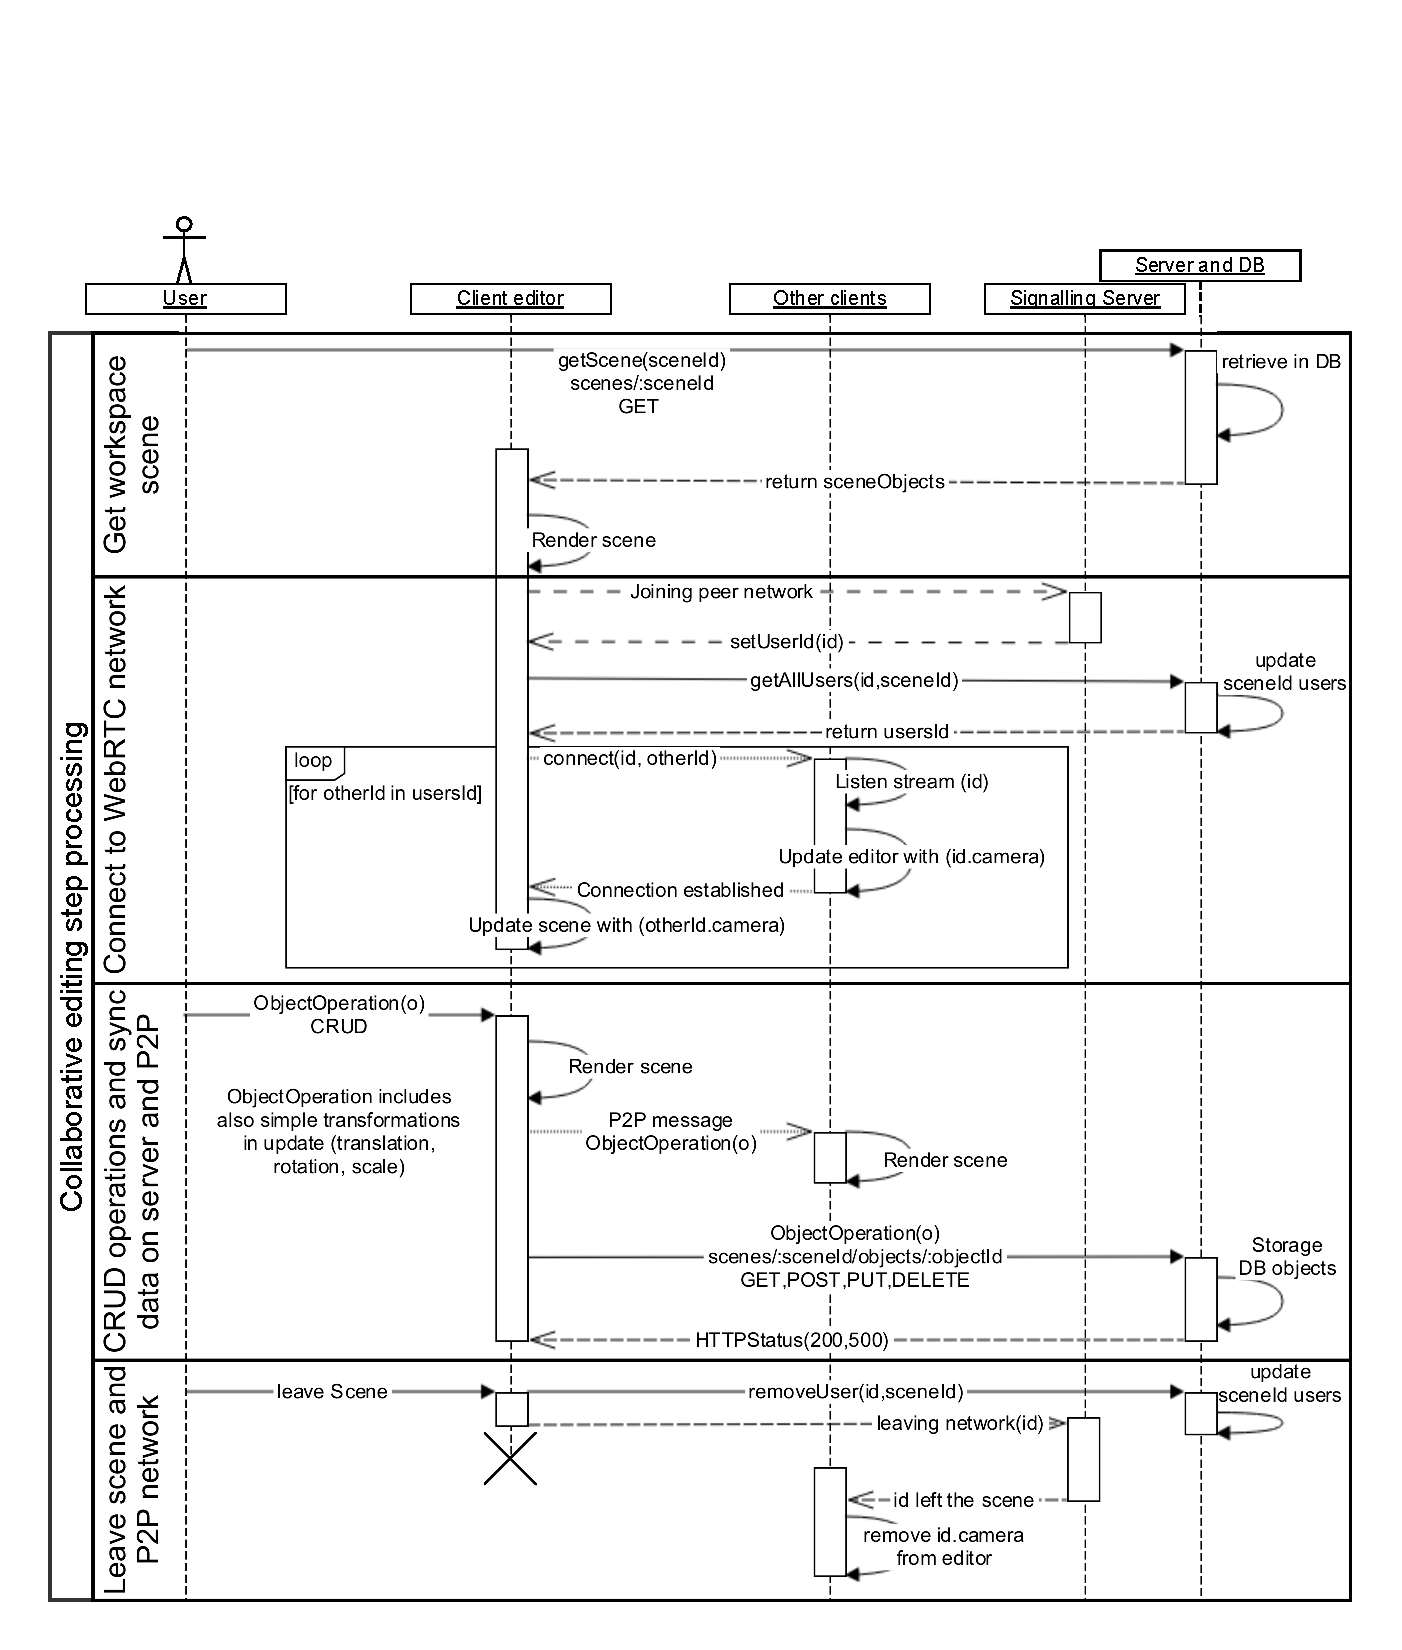
\includegraphics[trim={0 0 0 3cm},clip,width=1\columnwidth]
	{eps/sequence_wscg.eps}
	\caption{Diagramme de séquence de la gestion de la session dans une 
	architecture \og orientée état\fg{}}
	\label{fig:sequence_state}
\end{figure}

%
%We propose to auto connect users on a scene with a We- bRTC connection. As 
%each user send their ID to the database at their arrival, they also retrieve those 
%which where already present on the scene. We are able to cre- ate a full mesh 
%topology network in order to make them communicate the updates.
%
%Even if we have a full mesh topology, the P2P message layer is more similar 
%the 
%star topology. Indeed, the Fig- ure 2 shows the path of a sent message 
%operation 
%on the connection and it is only sent to the one degree neigh- bors of the original 
%broadcaster (the “B” node on the Figure 2).
%
%
%We choose to keep reliable and in order delivery for now. The RTCDataChannel 
%API supports many data types (strings, binary types: Blob, ArrayBuffer. . . ). 
%These types are helpful in a 3D multi user environment to broadcast messages 
%including the objets and their transformations. We tried to limit the amount of 
%data 
%by sending only relevant information but there is actually no particular 
%optimization. The channel can be over- feed when an object is imported then 
%pushed through the network.
%

\subsubsection{Gestion de la synchronisation et de la cohérence}
\label{sec:synchronisation-client-serveur}

Les travaux \cite{Desprat2015a} et \cite{Desprat2015b} présentent une version 
naïve du processus de synchronisation. La cohérence est garantie par un système 
de verrouillage des objets. Cela évite notamment les sélections concurrentes et par 
conséquent les éditions concurrentes. 
Lors de la récupération de la scène, elle est considérée comme cohérente. 
Ensuite, le choix d'avoir des connexions \gls{P2P} ordonnées et fiables, ainsi qu'un 
maillage de pair complet, implique que toute donnée envoyée par un pair est 
forcément reçue par les autres. 

Lors de la connexion d'un nouveau client, a lieu la synchronisation des deux 
systèmes de persistance pour obtenir les mises à jour : 
\improve{l'échange des mises à jour entre le client (persistance à court terme) et la 
	base de données (à long terme) afin de synchroniser les deux éléments avec. 
	La base de données peut également servir en cas de conflits importants ; elle sert 
	de référent.}
\begin{enumerate}
	\item depuis le client, où l'on distingue trois cas :
	\begin{enumerate}
		\item travail "\textit{offline}" (hors ligne) : l'utilisateur a travaillé hors ligne et 
		doit maintenant publier "en ligne" son travail. Les mises à jour sont publiées sur la 
		base de données ; le serveur vérifie si aucun conflit ne survient puis 
		fusionne (\textit{merge}) les nouvelles entrées avec l'existant; 
		
		\item travail "\textit{serverless}" (en collaboration avec entre pairs sans le 
		serveur) : dans le cas où le serveur est absent, les clients peuvent continuer 
		de créer en collaborant. Ces données n'étant stockées que sur le client, il est 
		nécessaire de les transmettre à la base de données dès qu'une connexion 
		est possible. 
		Cela peut être fait en une fois ou de manière partagée\improve{ça veut dire 
			quoi?};
		
		\item travail "\textit{online}" (en collaboration entre pairs comprenant la partie
		serveur) : le client envoie régulièrement \improve{combien de temps} ses 
		nouvelles modifications pour qu'elles soient intégrées à la base de données.
	\end{enumerate}
	\item depuis la base de données :
	Le client reçoit toutes les nouvelles mises à jour de la scène depuis la dernière 
	fois qu'il s'est connecté. Cela peut également inclure des mises à jour qui sont 
	en conflit avec ce qu'il y a dans son propre espace de stockage, qu'il lui faut 
	donc modifier.
	Dans le cas où un utilisateur est seul connecté, la base de données est la 
	seule source disponible pour la mise à jour du client. 
\end{enumerate}


Le fait de synchroniser un client avec une base de données NoSQL dès que cela 
est possible permet de supporter les connexions intermittentes comme pour les 
appareils mobiles dans cette architecture ; cette approche est connue sous le nom 
de \og\textit{offline first}\fg{} \cite{Gadea2016}.
\subsubsection{Topologie et protocole d'échange}
Cette architecture est basée sur une topologie de maillage complet (\textit{full 
mesh topology}) pour le réseau \gls{P2P}.
Les échanges se font donc à deux niveaux: entre les pairs, ainsi qu'entre chaque 
pair et la base de données. Pour le premier niveau, la couche réseau \gls{P2P} est 
assez 
naïve dans le sens où les connexions sont considérées comme fiables et 
ordonnées ; le client n'a alors qu'à publier toutes les modifications qu'il effectue et 
les envoyer à tous les clients (auxquels il est nécessairement connecté).
Les pairs échangent des différentiels d'état sur les objets. Ces messages ne 
contiennent pas d'information sémantique sur le type d'action effectuée par chaque 
utilisateur. 

\subsubsection{Discussion des problématiques liées à une architecture de 
communication orientée \og états\fg{}}

La base de données centralisée est beaucoup sollicitée lors des sessions 
collaboratives, ce qui peut mener à une surcharge similaire aux architectures 
uniquement client-serveur. 
En combinant client-serveur et \gls{P2P}, la charge aurait dû être réduite et 
transférée aux autres pairs, notamment lors de la phase de récupération d'une 
nouvelle scène qui repose entièrement sur le serveur. 
Chaque pair assume la responsabilité dans l'envoi de ses modifications à tous les 
autres pairs. Cette tâche ne profite pas du réseau \gls{P2P} de manière optimale 
car la topologie ne profite pas de la fonction relais des pairs. Cela pourrait alléger  la 
distribution dans la couche \gls{P2P} et responsabiliser un peu plus les pairs pour 
faciliter le passage à l'échelle.
En effet, la topologie en maillage complet limite le passage à l'échelle car le 
nombre de connexions va croître de manière exponentielle. 

Par ailleurs, les requêtes \gls{CRUD} ne sont pas très expressives concernant le 
métier. 
Aucune vérification n'est donc effectuée sur la validité des données transmises 
dans cette architecture. De plus, il peut arriver, du fait de latences réseaux que les 
modifications des différents utilisateurs s'entrelacent à l'arrivée et ne rendent pas 
l'intention de l'utilisateur. Cela peut mener à des dé-synchronisations fortes.

Concernant la gestion de la concurrence, l'utilisation d'une solution pessimiste 
dans un environnement \gls{P2P} peut parfois mener à des inter-blocages si un 
utilisateur quitte la scène sans avoir relâché l'objet, c'est à dire sans en avoir 
informé la base de données et les autres 
utilisateurs. 
Même si l'application peut prendre le relais et permettre la relâche du 
verrou au bout d'un certain temps, l'expérience utilisateur peut être dégradée 
pendant cette période.
Le maintien de la cohérence est a peu près garanti dans ce modèle si l'on 
considère un environnement où la fréquence des modifications n'est pas très 
élevée, et que tous les clients communiquent leur horloge locale pour établir un 
référentiel de temps concernant les mises à jour. 

Enfin, le transfert par différentiel d'état utilisé pour réduire la taille des 
données liées au changement d'état des objets lors de la transmission des 
données peut varier grandement selon le type de changement 
effectué, rendant peu prévisible la charge des canaux de communication. 
%
%Some issues remain in RTCDataChannel API : the com- patibility and 
%interoperability is still not complete be- tween browsers6, some browsers (like 
%Chrome) im- pose a send limit (about 6MB) for the data transmitting through 
%DataConnections and the security of the com- munication is still vulnerable7. 
%The 
%system overview (Figure 4) illustrates the communication architecture topology 
%between the peer clients and server (plus sig- naling).



%\subsection{De l'état à l'événement}
%\label{sec:statetoevent}

\subsection{De l'état à l'événement}
\label{sec:statetoevent}
Afin d'intégrer la notion d'historique dans une application web, plusieurs indicateurs 
sont nécessaires (version, granularité de l'historisation, type et taille des données 
manipulées). Cette section décrit le processus pour passer d'un système basé 
états à un système basé événements dans l'intérêt de réduire la somme des 
données transmises sans perdre d'information concernant la logique métier.
\paragraph{Description des variables}
Une scène $S$ contient l'ensemble des $n$ objets $x$ ($S =\{x_0,x_1,...,x_n\}$). 
Chaque élément de $S$ est associé à une taille calculée comme la somme des 
modifications $m$ selon la version $v$. 

Pour tout objet $x$ appartenant à la scène $S$ on associe une taille $w \in 
\mathbb{R}$. $w$ correspond à la taille totale des données transmises pour 
modifier l'objet à chaque version $v$ ($v$=0 correspond à la taille de l'objet à l'état 
original, i.e. l'\gls{EventStore} est vide). La taille totale de la scène, notée $Sw$, 
correspond à sommer la taille de tous ses objets (équation \ref{eq:sw}). Toutes les 
variables évoquées sont exprimées en octet pour avoir des termes avec des 
unités homogènes.

\begin{equation}
\label{eq:sw}
\text{Taille d'une scène $S$ : } S_w= \sum_{i=0}^{n}w_i
\end{equation}


\paragraph{Transmission par état}
Dans un système où à chaque modification on transmet l'état complet (équation 
\ref{eq:complet}), la taille des éléments transmis correspond à la somme de tous 
les états par lesquels l'objet est passé. Cette valeur va augmenter par paliers de 
tailles du même ordre de grandeur.
La transmission par état propose un historique issu d'une sauvegarde 
chronologique. Cependant elle est lourde voire redondante et n'offre pas 
d'information sur l'intention de l'utilisateur (quelle opération a permis d'arriver à cet 
état?).

\begin{equation}
\label{eq:complet}
\text{Par état : } w_i = \sum_{v=0}^{n}state_{v}
\end{equation}


\paragraph{Transmission par différentiel d'état}
\label{par:diff}
Dans un système où l'on transmet un différentiel d'état (équation 
\ref{eq:différentiel}), la différence entre deux états peut être difficile à exprimer (ex: 
MeshHisto \cite{Salvati2015})
car il s'agit d'un objet 3D dont les informations, stockées dans 
un fichier, ne sont pas linéaires. Le différentiel peut beaucoup varier jusqu'à 
atteindre une taille proche de l'état actuel si une transformation génère beaucoup 
de modifications par rapport à l'état précédent. A contrario, une modification sur la 
position d'un objet peut être très légère. La fonction représentant la taille des 
ressources transmises augmentera par palier avec au pire les propriétés de la 
proposition précédente (équation \ref{eq:complet}). Le différentiel d'état permet 
d'alléger la transmission par rapport à la proposition précédente, ne contenant 
cependant pas d'information sémantique sur ce qui est transmis et les opérations 
qui ont conduit à l'état d'un objet 3D de la scène.

\begin{equation}
\label{eq:différentiel}
\text{Par différentiel d'état : } w_i = state_0 + \sum_{v=1}^{n}(\underbrace{state_{v} 
- state_{v-1}}_{differential})
\end{equation}

\paragraph{Transmission par événement}
La transmission par événement (équation \ref{eq:evenement}) repose sur le 
principe du différentiel d'état ($differential$) exprimé ci-dessus (équation 
\ref{eq:différentiel}) en ajoutant la notion de type d'événement ($eventType$). Le 
type d'un événement indique le nom de la transformation à appliquer pour passer 
d'un état à l'autre. Un événement contient par nature une sémantique <<métier>> 
associée à chaque opération qui donne des indications sur l'intention de 
l'utilisateur. 

\begin{equation}
\label{eq:evenement}
\text{Par évènement : } w_i= state_0 + \sum_{v=1}^{n}(\underbrace{eventType + 
differential}_{event}) 
\end{equation}

Dans un \gls{EVC3D}, il y a des événements concernant à la fois la manipulation 
3D, la navigation et les éléments se rapportant à la collaboration (par exemple: 
prendre le point de vue d'un collaborateur). La taille d'un événement est variable 
(comme un différentiel d'état) avec un minimum contenant le type d'événement 
($eventType$) dû à sa structure type/paramètres. Cette proposition est un peu 
plus lourde à transmettre que la précédente mais ajoute une valeur sémantique à 
l'historique.



%\subsection{Architecture de communication \og orientée événements\fg{}}
%\label{sec:comm_event}

\subsection{Architecture de hybride \og orientée événements\fg{}}
\label{sec:comm_event}



\subsubsection{Persistance à long terme}\label{sec:persistance-a-long-terme}
Dans un contexte industriel de collaboration, l'information doit être disponible sur le 
long terme, facilement accessible par l'entreprise. La persistance à 
long-terme stocke le journal d'événement qui est la 
source de vérité de l'application. Elle peut également stocker des projections 
prédéfinies, calculées à la volée ou encore des \textit{snapshots} de l'application.



\subsubsection{Mécanisme de gestion de version}
3DEvent intègre une procédure de gestion de version dans l'\gls{EventStore} afin 
de gérer au mieux la cohérence des données. 
Chaque gestion de commande (Figure \ref{fig:gestionCommande}) entraîne la 
génération d'un ou plusieurs événements. Ces événements sont considérés 
comme \og soumis\fg{} (\textit{uncommitted}) mais pas encore <<~publiés~>> 
(\textit{committed}).  Pour qu'ils le deviennent, l'agrégat concerné par ces 
événements doit produire une nouvelle version sans être en conflit avec la 
précédente. En passant la version attendue $v_a$ au gestionnaire de conflit, on 
est à même de la comparer avec la version courante $v_c$. Il existe deux cas où 
un conflit est levé~: 
\begin{enumerate}[label=\alph*)]
	\item \label{i:vi} La version $v_a$ correspond à la valeur d'initialisation
	\item \label{i:vdiff} La version $v_a$ est différente de la version $v_c$
\end{enumerate}
Dans \ref{i:vi}, on s'assure qu'après une action la version initiale de l'agrégat ne 
peut être la même. Cet item peut sembler évident mais il est important de le noter 
car il dépend entièrement de la valeur initiale choisie pour les agrégats du 
\gls{framework} (on peut commencer à n'importe quelle valeur -- -1, 0\ldots).


%
%\subsubsection{Gestion de la cohérence}
%
%
%\subsubsection{Respect de la causalité}
%\subsubsection{Convergence des répliques}
%\subsubsection{Préservation de l'intention}
\subsubsection{Extension : Event Store distribué}


%\paragraph{Connexion des pairs en début de session}
Dans \cite{Desprat2017}, lorsqu'un pair initialise ou rejoint, la séquence pour 
rejoindre une session collaborative évolue 
pour prendre en considération l'intégration des événements et la synchronisation 
des journaux d'événements.
La Figure \ref{fig:connexionpairs} représente la séquence d'actions nécessaire à 
une instance 3DEvent ($idA$) pour rejoindre le réseau contenant déjà d'autres 
instances 3DEvent. L'action \textit{join} est exécutée lorsqu'un utilisateur envoie 
ses informations de connexion sur un portail de connexion (à partir d'une instance 
web) ou lorsqu'une instance serveur est lancée. Cette action ajoute le nouveau 
pair à la liste des pairs présents sur le réseau. La liste est gérée par le 
gestionnaire 
d'instance, et retourne la liste des pairs avec lesquels le pair doit se connecter. 
Pour chaque pair $idB$ de la liste retournée $ids$, $idA$ utilise le mécanisme de 
signalisation (offre/demande). Le mécanisme est déclenché par l'instanciation d'un 
\textit{network bridge}\info{definir} dans l'\textit{event store} \info{definir} de $idA$ 
puis celui de $idB$. Afin de resynchroniser les deux pairs (après cette série 
d'échanges asynchrones), $idA$ et $idB$ s'échangent des métadonnées sur la 
situation respective de leurs \textit{ESM} \info{definir} afin de se synchroniser 
\info{(see refernece sync mechanism}.

\begin{figure}[h]
	\noindent
	\centering
	\includegraphics[width=\columnwidth]{connection.eps}
	\caption{Protocole de connexion au réseau d'instance 3DEvent}
	\label{fig:connexionpairs}
\end{figure}



L'Event Store est un composant clé dans le traitement des événements. Il prend 
en entrée des événements générés ou reçus extérieurement et produit en sortie 
des événements cohérents qui peuvent être par la suite publiés. Les événements 
sont considérés comme cohérents lorsqu'il n'y a pas d'erreur de cohérence, i.e. 
lorsque les numéros de versions sont bien ordonnés. Chaque Event Store contient 
deux éléments: l'Event Stream Manager (ESM) et des Network Bridges (NB). Un
ESM est une structure de données représentée par une collection de flux 
d'événements. Un flux d'événement est représenté par un tableau d'événements 
indexés en séquence permettant de stocker les événements d'un aggrégat dans 
l'ordre temporel. Si un flux ne rencontre pas de problème de cohérence alors le 
dernier index correspond au numéro de version de l'agrégat. Lorsque l'Event Store 
reçoit un événement de l'instance courante\info{utilisation du terme 
	instance?}, l'ESM récupère (ou crée) le flux d'événements associé à l'agrégat 
référencé par l'événement. Alors, la cohérence de la version est vérifiée en 
comparant la version attendue (exposée dans les métadonnées de l'événement) 
et la version actuelle de l'agrégat. Si les deux numéros de versions sont égaux, 
l'événement est ajouté à la fin du tableau du flux pour être stocké, sinon une 
exception est levée. La gestion des exceptions est expliquée dans \info{détails 
	exception}. Une fois le stockage effectué dans l'ESM, l'événement est publié.


\subsection{Comparaison des deux architectures}

% Please add the following required packages to your document preamble:
% \usepackage{booktabs}
\begin{table}[h]
\centering
\caption{Récapitulatif des deux approches d'architecture de communication}
\label{ta:recap-approche}
\begin{tabular}{@{}lll@{}}
\toprule
\textbf{Critère}    & 
\textbf{HybridEvent}                                                                                      & 
\textbf{HybridState}                                                                                      \\ 
\midrule
Type stockage pair  & Fonctionnel 
(event)                                                                                       & 
Relationnel                                                                                               \\
Type BDD            & Fonctionnel 
(event)                                                                                       & NoSQL (Doc. 
JSON)                                                                                         \\
Cohérence           & 
Éventuelle                                                                                                & 
Forte                                                                                                     \\
Synchronisation     & 
Push-pull                                                                                                 & 
Push                                                                                                      \\
Gestion de conflit  & 
Flexible                                                                                               & 
Verrouillage des objets                                                                                   \\
Robustesse          & \begin{tabular}[c]{@{}l@{}}Plusieurs pairs sont liés \\ au 
serveur BDD : \\ disponibilité ++\end{tabular} & 
\begin{tabular}[c]{@{}l@{}}Lourde charge pour le \\ serveur lié à la BDD:\\ 
disponibilité - -\end{tabular} \\
Connectivité pair   & One-to-many 
(policy)                                                                                      & 
One-to-all                                                                                                \\
Passage à l'échelle & 
Oui                                                                                                       & 
Faible                                                                                                    \\
Orientée métier     & 
Oui                                                                                                       & 
Non                                                                                                       \\
Transmission        & Notification 
événement                                                                                    & Diff. 
état                                                                                                \\
Topologie Maillage  & 
Partiel                                                                                                   & 
Complet                                                                                                   \\
Type données        & 
Évènement                                                                                                 & 
État                                                                                                      \\
Type requêtes       & Projection / 
DTO                                                                                          & CRUD / 
REST                                                                                               \\
Historique des données         & 
Oui                                                                                                       & 
Non                                                                                                       \\
Défaire / Refaire   & Oui 
(compensation)                                                                                        & 
\begin{tabular}[c]{@{}l@{}}Oui (annulation commande \\avec effets de 
bord)\end{tabular}                \\ \bottomrule
\end{tabular}
\end{table}



\subsection{Bilan comparatif}
Le Tableau \ref{ta:recap-approche} propose un récapitulatif des deux approches 
utilisées. HybridEvent correspond à l'architecture hybride \og orientée 
événements\fg{} tandis qu'HybridState est l'architecture \og orientée états\fg{}.
Il est important de noter qu'HybridEvent a été conçue après HybridState et que les 
choix de modélisation ont évolué avec le temps. Globalement, HybridEvent a une 
approche très peu couplée par rapport à HybridState que ce soit concernant la 
connectivité, le type de transmission ou encore le mode de cohérence choisi.

HybridEvent propose une gestion des données mieux répartie compte tenu de la 
possibilité de \og composer\fg{} le réseau \gls{P2P} en fonction des besoins avec 
l'ajout à la volée de nouvelles instances Serveur. Cependant, le choix d'une 
synchronisation par les pairs rend la garantie de la cohérence plus complexe à 
faire aboutir contrairement à HybridState. Cette dernière consomme les 
ressources par à-coups alors qu'HybridEvent repose principalement sur la 
transmission de flux de données en continu.

% Please add the following required packages to your document preamble:
% \usepackage{booktabs}
\begin{table}[h]
\centering
\caption{Récapitulatif des deux approches d'architecture de communication}
\label{ta:recap-approche}
\begin{tabular}{@{}lll@{}}
\toprule
\textbf{Critère}    & 
\textbf{HybridEvent}                                                                                      & 
\textbf{HybridState}                                                                                      \\ 
\midrule
Type stockage pair  & Fonctionnel 
(event)                                                                                       & 
Relationnel                                                                                               \\
Type BDD            & Fonctionnel 
(event)                                                                                       & NoSQL (Doc. 
JSON)                                                                                         \\
Cohérence           & 
Éventuelle                                                                                                & 
Forte                                                                                                     \\
Synchronisation     & 
Push-pull                                                                                                 & 
Push                                                                                                      \\
Gestion de conflit  & 
Flexible                                                                                               & 
Verrouillage des objets                                                                                   \\
Robustesse          & \begin{tabular}[c]{@{}l@{}}Plusieurs pairs sont liés \\ au 
serveur BDD : \\ disponibilité ++\end{tabular} & 
\begin{tabular}[c]{@{}l@{}}Lourde charge pour le \\ serveur lié à la BDD:\\ 
disponibilité - -\end{tabular} \\
Connectivité pair   & One-to-many 
(policy)                                                                                      & 
One-to-all                                                                                                \\
Passage à l'échelle & 
Oui                                                                                                       & 
Faible                                                                                                    \\
Orientée métier     & 
Oui                                                                                                       & 
Non                                                                                                       \\
Transmission        & Notification 
événement                                                                                    & Diff. 
état                                                                                                \\
Topologie Maillage  & 
Partiel                                                                                                   & 
Complet                                                                                                   \\
Type données        & 
Évènement                                                                                                 & 
État                                                                                                      \\
Type requêtes       & Projection / 
DTO                                                                                          & CRUD / 
REST                                                                                               \\
Historique des données         & 
Oui                                                                                                       & 
Non                                                                                                       \\
Défaire / Refaire   & Oui 
(compensation)                                                                                        & 
\begin{tabular}[c]{@{}l@{}}Oui (annulation commande \\avec effets de 
bord)\end{tabular}                \\ \bottomrule
\end{tabular}
\end{table}

\section{Conclusion du chapitre}
Dans ce chapitre est décrit l'ensemble des contributions théoriques de la thèse. 
Dans un premier temps, le modèle événementiel propose une architecture 
complète permettant à un client d'intégrer les règles métiers liées à la manipulation 
et la visualisation d'objets 3D. Le modèle événementiel est utilisé pour traiter les 
événements à plusieurs niveaux : validation des données en fonction des règles 
métier, du stockage, de la détection de conflits interne et de la visualisation flexible. Tous 
ces aspects permettent d'ouvrir sur la deuxième contribution : 
l'architecture de communication hybride combinant client-serveur et \gls{P2P}.
Cette seconde partie se partage entre une architecture \og orientée états\fg{} et 
une architecture \og orientée événements\fg{}. Pour chacune de ces architectures, chaque composant est décrit en fonction des spécificités du paradigme utilisé. 

L'utilisation de la 
technologie WebRTC permet de proposer une 
architecture qui respecte les standards du web et l'interopérabilité nécessaire aux \glspl{EVC3D}. La mise en place d'une architecture décentralisée dans un 
environnement distribué permet de mettre à contribution tous les acteurs de la 
collaboration. De ce fait, l'accessibilité des ressources est renforcée par la 
présence de nombreuses unités sur le réseau. Cela permet à la fois 
de récupérer du contenu rapidement, et d'octroyer une autonomie aux 
contributeurs. 

Différentes problématiques liées à la cohérence et la synchronisation ont été 
évoquées. L'architecture semi-décentralisée proposée fournit plusieurs 
pistes pour la détection de conflits. Les choix effectués lors de l'implantation permettront d'analyser les différents échanges entre tous 
les composants de chaque modèle et de souligner les avantages et les 
inconvénients des choix de modélisation exprimés dans les contributions.


% ----- chapitre Implantation
%%!TEX root = main.tex

\chapter{Implantation}
\chaptertable

\section{Introduction} 
Cette section présente l'implantation de 3DEvent, la plateforme web de 
manipulation et visualisation collaborative d'objets 3D réalisée à partir du modèle 
présenté dans le chapitre précédent.

La première partie s'intéresse à l'intégration 
du framework pour proposer une application d'assemblage d'objets 3D. La 
présentation commence avec la description de l'\gls{IU} et des fonctionnalités 
proposées dont le principe de sélection fantôme et le système de visualisation 
flexible reposant sur le système de projection du modèle orienté événements. 

La seconde présente l'implémentation de l'architecture de communication avec les 
différentes implémentation des acteurs du système, les politiques de connexion et 
l'intergiciel \gls{P2P} qui permettent l'échange de données entre les collaborateurs.

Enfin, la troisième section récapitule et discute les choix techniques pour 
l'interface utilisateur et la partie réseau qui ont été fait dans l'implémentation.


\section{3DEvent : Plateforme web de manipulation collaborative d'objets 3D}
Dans le chapitre précédent une des contribution présentée correspond au 
modèle orienté événements : le \gls{framework} 3DEvent. 
Son implémentation prend la forme d'une application web qui intègre un éditeur 
pour la visualisation et la manipulation d'objets 3D de manière collaborative (aussi 
appelée \og application 3DEvent\fg{}).

%\chapter{Implantation}
%\section{3DEvent : Plateforme web de manipulation et visualisation 
%	collaborative 
%	d'objets 3D}
\subsection{Éditeur 3DEvent}
L'intérêt de proposer une application web se 
retrouve principalement dans 
l'accessibilité qu'elle propose. En effet, n'importe 
quel terminal muni d'un 
navigateur web peut y accéder, ce qui la rend distribuée et multi-plateforme. 
Les fonctionnalités graphiques proposées par WebGL sont un peu réduites par 
rapport à celles d'OpenGL dont l'\gls{API} évolue plus vite et propose plus de 
flexibilité et d'optimisations. Cependant, les performances graphique restent très 
correctes car le navigateur est quand même capable d'utiliser les processeurs 
graphiques du terminal (GPU) pour les calculs et rendus \gls{3D}.

Pour faire le lien entre le modèle et l'expérimentation, l'implantation du modèle a 
pris la forme d'un éditeur pour la modélisation \gls{3D} haut niveau permettant de 
visualiser et manipuler des objets \gls{3D} de manière collaborative dans un 
environnement web (aussi 
appelée \og application 3DEvent\fg{}). Au sein de la plateforme, les interactions 
possibles sont : 
\begin{description}
	
	\item[Visualiser, naviguer, utiliser les outils de transformation] L'utilisateur peut, 
	com\-me dans un environnement \gls{3D} classique, interagir avec la vue en 
	utilisant 
	la souris (survol, clic) et en bougeant la caméra (déplacements). Il peut 
	utiliser les commandes clavier et souris pour effectuer des opérations de 
	translation, de rotation et d'homothétie de trois manières différentes: directement dans le \textit{viewport}, via le 
	menu ou via la console du navigateur.
	\item[Charger des modèles \gls{3D}] L'éditeur gère la plupart des formats de 
	fichier 
	3D \info{ref [Bou12]}(OBJ, PLY, DAE, glTF\ldots)
	\item[Changement de référentiel] La modification des coordonnées de 
	réfé\-ren\-ces (local/global)  pour les différentes transformations possibles
	\item[Grid snapping] Cette fonctionnalité permet d'aligner les modèles avec la 
	grille avec un effet de magnétisme sur les intersection de la grille.
	\item[Changement de point de vue] L'utilisateur peut à tout moment passer de 
	son point de vue à celui d'un autre utilisateur. Le choix d'implanter ce type de 
	fonctionnalité s'inscrit dans la perspective de sensibilisation de l'utilisateur au 
	travail de ses collaborateurs. Ainsi, lors de la session, le fait de prendre le 
	point de vue d'un collaborateur est une manière de 
	comprendre son fonctionnement et d'imaginer ses 
	perspectives de conception à travers son angle de caméra qu'il a choisi.
\end{description}



\subsection{Interface utilisateur orientée tâche}

Dans le but de proposer une \gls{IU} proche des fonctionnalités métiers liées à la 
modélisation \gls{3D}, l'éditeur possède une interface orientée \og tâche\fg{}, en 
comparaison avec des \gls{IU} \gls{CRUD}. En effet, les \gls{IU} \gls{CRUD} 
réduisent la sémantique métier du domaine d'application à la création, la lecture, la 
mise à jour et la suppression, omettant toutes les subtilités que peuvent dégager 
ces actions en perdant l'intention de l'utilisateur dès le niveau de l'interface. Une 
interface orientée tâche a tendance à s'attarder sur toutes les nuances que le 
domaine possède en caractérisant chaque action sans subir d'effet de 
simplification. Cette proximité avec le métier permet de calquer directement 
l'interface du modèle événementiel sur l'\gls{IU} et de guider l'utilisateur dans ses 
activités. L'utilisabilité, qualité de l'expérience utilisateur fournit par un système 
pour réaliser une tâche, est alors maximisée en terme d'efficacité, d'efficience et 
de satisfaction. 
Ce type d'\gls{IHM} s'organise autour de cas d'utilisation. Cela permet, 
d'une part, de présenter clairement les 
actions (\og ajouter une géométrie à la 
bibliothèque à partir d'un fichier\fg{} plutôt que \og téléverser un fichier\fg{}) : 
l'intention est clairement définie. D'autre part, lorsque l'utilisateur s'apprête à faire 
une action, seules les informations utiles sont affichées. Enfin, l'application fournit 
simplement l'information dans le contexte où elle doit être présentée, évitant à 
l'utilisateur d'aller la chercher ailleurs.
L'\gls{IU} devient alors une couche de l'application qui nécessite d'agréger, croiser 
et filtrer des données. La dénormalisation proposée par \gls{CQRS} remédie à ce 
besoin dans le cadre de la consultation de données. 


\subsubsection{Présentation de l'interface}


%\begin{figure}[h!]
%	\centering
%	\begingroup
%	
%	\subfloat[Rotation (vue \gls{3D}) et outils de manipulation d'objet 
%	\gls{3D} 
%	(panneau 
%	
%latéral)]{\includegraphics[width=0.75\textwidth]{eps/2rotatedetail.eps}\label{fig:ui2}}\hfill
%	
%	\subfloat[Translation (vue \gls{3D}) et visualisation de l'historique 
%	(panneau 
%	
%latéral)]{\includegraphics[width=0.75\textwidth]{eps/1translatehisto.eps}\label{fig:ui1}}\hfill
%	
%	\subfloat[Mise à l'échelle (vue \gls{3D}) et liste des collaborateurs 
%	(panneau 
%	
%latéral)]{\includegraphics[width=0.75\textwidth]{eps/3scalecollab.eps}\label{fig:ui3}}\hfill
%	
%	\endgroup
%	\caption{Interface utilisateur pendant une session collaborative (trois 
%personnes)}
%	\label{fig:screenshots}
%\end{figure}
Lorsqu'un utilisateur se connecte à une scène, il a accès à une interface web 
(dans un navigateur) qui représente l'espace de travail collaboratif lui permettant 
d'utiliser différentes fonctionnalités. Les deux modalités d'interaction sont le clavier 
et la souris\info{est ce qu'on parle de mobile?}. Le premier niveau de cette 
interface est scindée en deux panneaux~: 
\begin{enumerate}
	\item L'espace \gls{3D} consacré à la visualisation des objets et à leur 
	manipulation 
	dans l'environnement \gls{3D}~;
	\item La barre d'outils qui contient trois onglets~:~
	\begin{enumerate}
		\item "Scene" contient tous les détails de la scène et des maillages qu'elle 
		inclue~; 
		\item "Collaboration" fournit les informations liées à la collaboration~;
		\item "History" liste tous les événements qui ont eut lieu dans la scène et 
		leurs  détails. 
	\end{enumerate}
\end{enumerate}

\begin{figure}[ht]
	\centering
	\begingroup
	
	\subfloat[Onglet \og outils de manipulation sur la 
	scène\fg{}]{\includegraphics[width=0.38\textwidth]{eps/scenecontrol.eps}\label{fig:uicontrol}}
	\hfill
	\subfloat[Onglet \og collaboration\fg{}]
	{\includegraphics[width=0.27\textwidth]{eps/collaboration.eps}\label{fig:uicollab}} 
	\hfill
	\subfloat[Onglet \og 
	historique]{\includegraphics[width=0.32\textwidth]{eps/history.eps}\label{fig:uihisotry}}
	
	\endgroup
	\caption{Onglets du panneau latéral de l'interface}
	\label{fig:uipanneau}
\end{figure}
La Figure \ref{fig:uipanneau} montre quelques captures d'écran durant une 
session collaborative sur le modèle Rotor.

L'onglet "Scene" (Figure \ref{fig:uicontrol}) possède un bloc contenant les détails 
d'un 
maillage en cours de 
sélection. Cela permet d'avoir la description des propriétés de l'objet sélectionné et 
une manipulation de ses paramètres (position, rotation et mise à l'échelle) plus 
précise que via l'espace \gls{3D} avec le cliqué / déplacé. "Scene" intègre 
également un espace réservé aux géométries disponibles dans la scène appelé 
Bibliothèque (de géométries).

L'onglet "Collaboration" (Figure \ref{fig:uicollab}) présente la liste des 
collaborateurs qui 
participent à la 
scène. Chacun d'eux est décrit par son nom, son état  (connecté ou déconnecté) 
et son rôle (administrateur, éditeur, lecteur ou autre\footnote{Un rôle peut être 
défini par le biais du \gls{framework} 3DEvent}). En cliquant sur un élément de la 
liste, l'utilisateur accède au dernier point de vue dans l'espace \gls{3D} connu du 
collaborateur représenté.

L'onglet "History" (Figure \ref{fig:uihisotry}) liste tous les événements passés dans 
la 
scène en fournissant 
l'accès à leur détail. Pour chaque événement, le système est capable de montrer 
dans l'espace \gls{3D} la différence entre l'état  après l'événement cliqué $state_x$ 
et l'état courant $state_n$. L'utilisateur peut à partir de cette visualisation choisir 
de \og revenir en arrière\fg{} sans perdre les données entre $state_n$ et $state_x$ 
car dans notre système cela s'effectue par compensation (cf Event-Sourcing 
Section X)\improve{annulation d'un événement ou juste ES}.

Dans chaque onglet se trouvent différents blocs \gls{HTML}, avec des 
comportements spécifiques à un agrégat et injectés dynamiquement. Ces blocs 
correspondent aux Views de notre modèle.

Les boîtes englobantes représentent la sélection des différents collaborateurs 
pendant la session.

Parmi les Views disponibles dans le système, une grande partie est dédiée à 
l'\gls{IU} de l'application web pour le cas d'utilisation de la modélisation 3D. 
D'autres Views sont disponible pour un autre cas d'utilisation destiné à 
l'observation des comportements des utilisateurs qui est primordiale dans le cadre 
des expérimentations.



\paragraph{Exemple d'interaction}
La Figure \ref{fig:cqrs-example} décrit la façon dont le système traite l'exécution 
d'une commande de translation déclenchée par l'utilisateur et comment cette 
information est diffusée à ces collaborateurs\footnote{Pour que l'exemple 
fonctionne, la scène, la géométrie du cube et le maillage \textit{cube1} doivent 
avoir été créés en amont.}.
Dans l'étape (a), la commande déclenchée par l'utilisateur s'adresse à l'agrégat 
$cube1$ et contient les paramètres de la translation (vecteur x,y,z). L'agrégat qui 
modélise le domaine d'un maillage, génère l'événement de translation $e1$ (étape 
(b)) si tout est valide d'un point de vue métier. L'événement $e1$ est ensuite 
passé à l'Event Store. 
Le composant responsable de la détection de conflit permet au développeur 
d'implémenter ses propres règles de résolution de conflit. Le composant déclenche 
une exception lorsque le numéro de version reçu et le numéro de version courant 
de l'agrégat sont identique (Figure \ref{fig:cqrs-example} étape (c)). Selon les 
règles métiers définies et les exceptions liés à la cohérence, l'événement peut être 
rejeté. Ce traitement peut être à l'origine de la génération de nouveaux 
événements.


\begin{figure}[]
	\centering
	\includegraphics[width=\columnwidth]{eps/example10.eps}
	\caption[Flux de la collaboration dans le framework 3DEvent entre 3 
	utilisateurs]{Exemple d'édition collaborative où User A est connecté à User  B, 
		lui 
		même connecté à User C. Le cycle montre les différentes étapes du 
		déclenchement de la commande au rendu visuel en passant par la 
		génération 
		de l'événement, la 
		synchronisation du journal d'événements et l'impact sur le rendu des autres 
		utilisateurs pour une translation sur un cube.}\label{fig:cqrs-example}
\end{figure}
\subsection{Flexibilité de la visualisation}
\label{sec:flexviz}
Dans l'approche \gls{CQRS}, une projection est définie comme une dérivation de l'état courant à 
partir du flux d'événements. Pour Abdullin, \og la projection est le processus de 
conversion (ou d'agrégation) d'un flux d'événement en une représentation 
structurelle. Cette dernière (qui est mise à au moment où le flux est parcourue) 
peut être avoir différentes appellations : modèle de lecture persistent, vue ou 
état\fg{}\cite{Abdullin2011}.
La partie lecture du modèle (l'affichage sur interface utilisateur) bénéficie des 
projections en lui permettant de réduire l'afflux des événements, ne laissant filtrer 
que ceux qui sont pertinents pour la vue. La projection fournit une vue adaptée 
(filtrée, enrichie\ldots) du flux d'événements au client. Elle peut également être 
utilisée pour mettre en avant des aspects experts (notifications, déclenchement 
d'action) ou des raisons de confidentialité.
Une projection peut être créée de manière synchrone (à la volée) au fur et à 
mesure de la publication des événements ou de manière asynchrone et donc 
découplée du flux des événements. 


Du fait de la nature d'un réseau \gls{P2P}, les pairs ne reçoivent pas forcément les 
paquets réseau de manière ordonnée.
Par conséquent, les messages peuvent arriver dans n'importe quel ordre.
Qu'arriverait-il alors si un événement A ($eA$) nécessitant un autre événement B ($eB$) arrivait avant celui-ci? Dans cette situation, le système génére une 
erreur en essayant d'appliquer $eA$ sur un état inadéquat car il n'a pas 
d'information sur la hiérarchie d'application des événements ($eB$ puis $eA$).

Pour pallier ce problème, l'introduction du système de projection permet d'avoir un 
mécanisme (comme un automate fini) qui défini les transitions nécessaires pour 
passer d'un état à l'autre. Les transitions réalisent les actions déterminées en fonction des 
événements qui arrivent. Par exemple, si on essaie d'ajouter un objet dans une 
scène  ($eA$) sans avoir créer la scène ($eB$) la projection met en attente $eA$ 
jusqu'à recevoir $eB$. Dans le cas où $eB$ n'arrive jamais, la projection ne pourra 
jamais utiliser $eA$.

\begin{figure}
	\centering
	\inputTikZ{0.9}{eps/tikz/streams/aggregate.tex}
	\caption{Exemple d'agrégats}{Structure d'un agrégat et ses versions. Chaque 
	version est un état de l'agrégat qui correspond à l'empilement des instances 
	d'événements (ei) qu'il contient. Les types des événements sont relatifs au type 
	d'agrégat dans lequel il est contenu.}
	\label{fig:aggregate}
\end{figure}

\paragraph{Projections}
chaque partie de l’interface est liée à une proj de la bdd
les actions user et les actions des autres users passent par le meme cycle
pas de diff de prise en compte des evnts de l’interaction user ou de la couche 
reseau
en CS : les actions users -> actions -> recup info
action push du servuer qui peuvent etre gerees de maniere diff
\subsection{Bilan}

 L'application 3DEvent repose sur les principes et les 
technologies du web pour permettre de visualiser et manipuler des objets \gls{3D} 
de 
manière 
collaborative en temps-réel.

\section{Intergiciel P2P pour l'échange de données 3D pour le paradigme 
événementiel}

L'architecture de communication décrite dans le chapitre précédent nécessite 
l'implémentation d'un intergiciel \gls{P2P} compatible avec les besoins liés à la 3D, le 
web et la collaboration. Cette section décrit les politiques de connexion pour 
l'éditeur présenté dans la section précédente ainsi que les mécanismes de 
synchronisation nécessaire à l'échange de données dans l'application. 

%!TEX root = main.tex
%\chapter{Implantation}
%editeur...
%\section{Intergiciel P2P pour l'échange de données 3D}
%\subsubsection{La virtualisation des clients}
%\label{virtualisation}
%\todo{mettre ailleurs?}
%Une des problématiques soulevée par la collaboration \gls{P2P} est de permettre 
%la reproductibilité des expérimentations dans un environnement contrôlé et 
%réaliste.
%Réussir à simuler un réseau virtuel de clients en \gls{P2P} en utilisant le 
%protocole 
%\gls{WebRTC} est un défi encore compliqué. Il existe des outils pour simuler des 
%réseaux \gls{P2P} tels que PeerSim \cite{Montresor2009} ou \textit{ns-3} 
%\cite{Riley2010}. Ces outils sont 
%plus orientés sur la façon de distribuer les informations lors de la simulation et 
%leur 
%dissémination au sein du réseau plutôt que de reproduire les protocoles et 
%l'infrastucture de manière réaliste avec des données issues de l'\gls{IU}. Dans 
%de 
%récents travaux utilisant \gls{WebRTC}, les expérimentations ne 
%sont pas encore facilement reproductibles du fait qu'il n'existe pas d'outil facile à 
%prendre en main pour effectuer ce genre de simulation à base d'entrées 
%utilisateur 
%fiables vis à vis des impératifs métier. 
%
%La virtualisation implique également de pouvoir simuler des comportements sur 
%la base d'interactions issues de \gls{IU} \cite{Hu2017} comme on peut le trouver 
%dans la simulation d'\gls{IU} web.
%Dans ce contexte, ce type de tests permet de vérifier la compatibilité et la 
%réactivité des différentes plateformes, versions de navigateurs et types 
%d'appareils 
%en fonction d'entrées utilisateur. C'est également utile pour faire des tests de 
%performance ou de montée en charge 
%concernant l'interface. 
%Le service testRTC\footnote{\url{testrtc.com}. Consulté le 
%	07/07/2017} est un service payant qui propose un outil de test et de monitoring 
%pour un grand banc de machines de sessions audio et vidéo WebRTC .
%
%
%%TODO mettre ailleurs?
%L'intérêt d'utiliser un modèle de réseau \gls{P2P} virtuel comporte plusieurs 
%avantages. En reprenant les points proposés par \cite{Haque2016}, on peut citer 
%: 
%\begin{itemize}
%	\item Pas d'installation nécessaire. Plusieurs outils et logiciels existent pour 
%	simuler des réseaux \gls{P2P} \cite{Montresor2009} ou nécessite encore 
%	l'installation de clients lourds (clients BitTorrent) par les utilisateurs pour 
%réaliser 
%	les mesures. Cela implique le fait de comprendre les principes de base 
%	concernant la configuration réseau (routeurs, pare-feu) et le protocole utilisé 
%	(BitTorrent). Très peu de travaux concernant \gls{WebRTC} ont réussi à 
%	virtualiser les clients participants aux expérimentations.
%	\item Opérabilité et interopérabilité dans un environnement contrôlé.  
%	L'installation d'un client sur une machine requiert certaines autorisations liés à 
%	la politique de l'organisation, la licence logicielle et le support logiciel. Ce type 
%	d'environnement est assez typique dans l'industrie, c'est pourquoi il est 
%	intéressant de proposer un modèle qui puisse s'exécuter sans difficulté grâce 
%à 
%	l'utilisation de clients web. Les navigateurs qui servent de clients web 
%	s'accordent généralement avec les standards proposés par le \gls{W3C}, ce 
%qui 
%	facilite également l'interopérabilité du logiciel souvent déployé dans un parc 
%	hétérogène de machines.
%	\item Indépendance de la situation géographique. Tout comme les 
%	infrastructures \textit{cloud} (souvent un service tiers) qui sont distantes par 
%	l'intermédiaire d'un réseau , généralement internet les utilisateurs peuvent se 
%	connecter sur un réseau virtuel  \gls{P2P} à partir de n'importe quel lieu. 
%	\item Simplification de la maintenance. Les applications, standards et 
%	protocoles autour du \gls{P2P} sont en constante évolution. L'implémentation 
%de 
%	la méthode de distribution des données nécessite par conséquent de 
%fréquente 
%	mises à jour pour être la plus efficace possible. Dans le cas d'une 
%	implémentation d'un client virtuel, la mise à jour qui est distribuée par le 
%serveur 
%	sera automatique et la même sur tous les clients ce qui facilite la 
%maintenance 
%	car c'est le distributeur qui est responsable de la mise à jour et non le client.
%	\item Mobilité et accès au réseau. La mise en place d'un réseau P2P permet 
%de 
%	découpler l'accès à l'information et aux ressources du système. De ce fait, 
%	les clients peuvent travailler directement entre eux sans supervision après 
%mise 
%	en relation et partager leurs ressources avec les autres clients qui en ont 
%	besoin. Le réseau peut évoluer sans que cela ait un fort impact sur la 
%	collaboration. Les clients peuvent être plus mobiles du fait de la grande 
%	disponibilité offerte par cette architecture à moindre coût.
%	\item \gls{NATT} et pare feu. Les applications traditionnelles de P2P comme 
%	BitTorrent ne permettent pas à deux pairs de communiquer directement 
%	lorsqu'ils sont derrière un \gls{NAT}. Grâce à l'utilisation du protocole \gls{ICE} 
%	les appareils peuvent atteindre plus de pairs, augmentant la vitesse d'échange.
%\end{itemize}
%
%Cette liste est un point de départ pour créer un service de virtualisation de 
%clients 
%pour le partage de données (3D) avec WebRTC. 
%La mise à disposition volontaire de ressources (calcul, mémoire) en partage sur 
%le 
%réseau permet d'une part la coopération entre personnes afin de résoudre des 
%problèmes nécessitant un haut degré de computation et d'autre part l'utilisation 
%de 
%ressources qui ne seraient pas ou sous utilisées.
%
%
%
%
%En 2001, le standard \gls{DDS} est un standard machine-à-machine massif, en 
%temps-réel, hautement performant avec un système d'échange de données 
%interopérables. \gls{DDS} s'adresse principalement à des problématiques 
%d'échanges financiers, de contrôle aérien, et de réseau électrique intelligent 
%(\textit{smart grid}). Il a fortement été promu pour mettre en place des 
%applications 
%liées à l'internet des objets. Les spécifications proposent deux niveaux 
%d'interfaces. Le premier se concentre sur la mise à disposition d'un système 
%\gls{PubSub} bas niveau centré données pour permettre la livraison efficace de 
%la 
%bonne information au bon destinataire. Le second, niveau optionnel, 
%est une couche de reconstruction locale de la donnée permettant une integration 
%plus simple de \gls{DDS} au sein d'une application. \gls{DDS} est donc un 
%intergiciel réseau basé sur une architecture \gls{PubSub} qui gère la livraison 
%de messages sans nécessiter l'intervention d'un utilisateur. Il détermine qui doit 
%recevoir les messages, où sont situés les destinataires et ce qu'il se passe si 
%un 
%message n'est pas délivré. En cela, \gls{DDS} permet une gestion plus fine de la 
%qualité de service notamment concernant les paramètres de découverte des 
%pairs.



L'assomption est faite que tous les clients utilisent des navigateurs qui 
implémentent et supportent le protocole WebSocket et l'\gls{API} 
RTCDataChannel. 

La topologie de l'architecture de communication repose sur la mise en relation 
automatique des clients par le biais du serveur pour établir une connexion 
\gls{WebRTC}. Pour ce faire, chaque client envoie son identifiant (ID) lors de sa 
première requête au serveur qui le stocke. Selon le paramétrage de la connectivité 
directe minimum établie préalablement, le serveur recherche aléatoirement l'ID 
d'autres clients qui satisfont la règle de connectivité. Cette règle de connectivité 
minimum permet d'ajuster la densité du maillage (connectivité élevée: maillage 
partiel dense, voire complet ; connectivité faible: maillage partiel éparse) et 
d'obtenir une topologie maillée adaptée aux besoins de l'application en termes de 
synchronisation (temps-réel ou non) ou aux capacités des appareils. Il faut noter 
cependant que plus la connectivité est faible, plus l'information a besoin de transiter par des intermédiaires pour atteindre tous les pairs et par conséquent le temps de 
transmission est augmenté (exemple d'une distribution en ligne). 

\subsubsection{Implantation du serveur}
La connexion entre un pair (client) et le serveur est établie sur la base du protocole 
\gls{WebSocket}. Cette connexion bi-directionnelle est initialisée lors de la 
première requête du client pour récupérer le contenu de l'application. Cette 
connexion sert à la fois pour la phase de \textit{signaling} lors de l'établissement 
d'une connexion \gls{WebRTC} mais également pour que le client puisse envoyer 
des mises à jours originales à la base de données via les pairs reliés à la base de 
données. 

Lors de la phase de \textit{signaling} c'est donc la partie gestion des instances du 
serveur qui gère la politique de connexion des données. Dans le prototype réalisé 
la connectivité minimum entre les différents pairs participant à la même scène est 
fixée à 2. Cette politique permet de créer un maillage réseau qui n'est pas trop 
dense en considérant que le nombre maximum d'utilisateur dépassera pas dix.



\subsubsection{De navigateur à navigateur}
Lors de la connexion d'un nouveau client à la scène, le serveur effectue la phase 
de \textit{signaling} permettant de le mettre en relation avec un autre client. Le 
mécanisme est répété tant que la règle de connectivité peut s'appliquer. Le client 
reçoit une notification de l'établissement de la connexion avec un autre client ce 
qui lui permet de démarrer l'échange de données.

L'API RTCDataChannel permet à chaque pair d'échanger des données arbitraires 
avec d'autres à partir du navigateur avec des propriétés de livraison 
personnalisables -- fiable ou non fiable (Section \ref{sec:fiabilite}), ordonné ou non 
ordonné (Section \ref{sec:ordre}). 

Dans 3DEvent, le choix d'avoir un transport 
fiable et non ordonné a été fait pour respectivement 
garantir l'arrivée d'une donnée émise par l'utilisateur au sein de l'application et 
permettre des échanges asynchrones.
\improve{add \S sur "en cas de défaillance? }
En cas d'arrêt soudain du serveur, si une connexion a été établie préalablement 
entre les clients et est toujours en cours, elle n'est pas impactée par la défaillance 
du serveur.

\subsection{Données d'échange}
En sachant que le modèle est conçu pour des applications web, 3DEvent a besoin 
d'un format de données permettant de faire communiquer des acteurs hétérogènes 
du système.
Le format \gls{JSON} est assez générique pour être aussi utilisé pour lors de la 
sérialisation et la désérialisation des 
événements et plus largement des paquets transmis par RTCDataChannel. 
L'\acrshort{API} RTCDataChannel supporte beaucoup de types de données 
différents (chaînes de caractères, types binaires : Blob, ArrayBuffer\dots). Dans 
un environnement multi-utilisateurs tel que 3DEvent avec des données 
hétérogènes (3D, images, 
informations) l'interopérabilité est facilitée.

Le Listing  \ref{jsonstore} représente la structure de données utilisée sur le réseau 
lorsqu'un événement est transmis. Seule la partie $data$ est utilisé au sein du pair 
pour faire les manipulations en \gls{CQRS} car le type de l'instance d'événement 
manipulé est connu. 

La structure représentant l'événement transporte un numéro de version \og 
attendue\fg{} 
qui correspond à la version que l'agrégat doit avoir lorsque l'événement lui est 
appliqué. De cette manière la cohérence interne du pair est maintenu grâce à ce 
numéro de version.
Les événements contenant les objets 3D ($importGeometryEvent$) ont une 
propriété contenant la géométrie sous la forme d'un Blob contenant le fichier. 
\\


%\begin{lstlisting}[language=json,firstnumber=1,label=jsonevent,caption=Événement
% MeshAddedToScene et ses paramètres]
%{
%	{
%		"sceneId": "scene-turbine",
%		"meshId":"406514c6-306b-f0f9643a037e",
%		"geometryId": "37076875-ea1c-bbd300481345",
%		"name": "blade",
%		"color": "#963912",
%		"version": 17,
%		"author": "Foo"
%	}
%}
%\end{lstlisting}

\begin{lstlisting}[language=json,firstnumber=1,label=jsonstore,caption=Format
 du Message transitant sur le réseau contenant l'événement MeshAddedToScene 
et ses 
paramètres]
{
	"packetId" : "567826g6-766b-f0g9676b677r",
	"streamId" : "scene-turbine",
	"eventType" : "MeshAddedToSceneEvent",
	"version" : 17,
	"data" : {
		"sceneId": "scene-turbine",
		"meshId":"406514c6-306b-f0f9643a037e",
		"geometryId": "37076875-ea1c-bbd300481345",
		"name": "blade",
		"color": "#963912",
		"author": "Foo"
	}
}
\end{lstlisting}

%\begin{lstlisting}[language=json,firstnumber=1,label=jsonexemple,caption=Format
%de l'événement MeshAddedToScene stocké dans la base de données Event 
%Store]
%{
%	"eventId": "9935bfa5-542e-2a44-add0-d3fb1abb7488",
%	"eventType": "MeshAddedToSceneEvent",
%	"eventNumber": 230,
%	"data": {
%		MeshAddedToSceneEvent : {
%			"sceneId": "scene-turbine",
%			"meshId":"406514c6-306b-f0f9643a037e",
%			"geometryId": "37076875-ea1c-bbd300481345",
%			"name": "blade",
%			"color": "#963912",
%			"version": 17,
%			"author": "Foo"
%		}
%	},
%	"streamId": "scene-work_living_room",
%	"positionEventNumber": 17,
%	"positionStreamId": "scene-work_living_room",
%	"title": "23@scene-work_living_room",
%	"id": "http://127.0.0.1:2113/streams/scene-work_living_room/17",
%	"updated": "2017-03-05T22:04:33.982814Z"
%}
%\end{lstlisting}
\subsection{Synchronisation des données}
\subsubsection{Persistance à court terme}
Le navigateur (client) offre un espace de stockage avec l'interface \textit{Storage} 
de l'API Web Storage qui donne accès au \texttt{session storage} ou au  
\texttt{local storage}. Ce stockage est présent sur le client et fonctionne sur un système de clé / valeur. La configuration du client est également 
stockée localement. Grâce à ce système, il est possible d'avoir une 
persistance des données à travers les sessions du navigateur. Le contenu stocké 
correspond aux données générées par un utilisateur et par ses collaborateurs. Les 
répliques stockées sur chaque navigateur permettent à un utilisateur une plus 
grande 
autonomie en cas de déconnexion. C'est également un moyen de distribuer entre les clients les 
mises à jour qu'ils génèrent grâce au protocole de 
\gls{streaming3D} (cf. \ref{streamingprotocol}) sans passer par le serveur.

événements enregistrés sur le client. La configuration du client est également 


\subsubsection{Protocole de streaming pour la synchronisation}
\label{streamingprotocol}

Il existe plusieurs méthodes de transmission de contenu au sein d'un réseau 
\gls{P2P} que l'on peut catégoriser selon deux modes : le téléchargement 
(\textit{download}) 
et le flux continu (\textit{streaming}). Le téléchargement requière que le contenu 
soit entièrement téléchargé pour pouvoir être lu, tandis que le flux continu peut 
être lu au fur et à mesure de sa récupération. Ce dernier mode, principalement 
utilisé pour la lecture de vidéo en ligne, s'applique bien à la transmission de 
contenu \gls{3D} : niveaux de détails \cite{Chu2012,Hu2008}, progressif 
\cite{Cheng2009,Limper2014}, mise en cache \cite{Jia2014}, compression / 
décompression
\cite{Lavoue2013,Ponchio2015,Maglo2013a}. 
Une catégorisation plus précise du flux continu peut être donnée selon quand le 
contenu est généré : 
en direct (\textit{live} ou \textit{push}) et à la demande (\textit{on-demand} ou 
\textit{pull}).  


Le mécanisme de routage que nous avons utilisé dans \cite{Desprat2015a} est 
proche du routage de GNutella. 





pour chaque event sauvé , l’Event store publie (push) l’event

\begin{algorithm} % enter the algorithm environment
	\caption{Sauvegarde d'événements d'un agrégat dans l'Event Store} % 
	%give the algorithm a caption
	\label{algo:saveEvent} % and a label for \ref{} commands later in the document
	\begin{algorithmic} % enter the algorithmic environment
		\REQUIRE aggregateId : string, uncommitedEvents : eventMsg[ ], 
		version : number
		%\ENSURE $y = x^n$
		\STATE $expectedVersion \Leftarrow version$
		\FOR{$eventMsg $ \textbf{in} $uncommitedEvents$}	
		\STATE{$newMsg \Leftarrow \{type : eventMsg.typeEvt, data : eventMsg, 
streamId : aggregateId\}$}
		\STATE{$publish(aggregateId, newMsg, expectedVersion++)$}
		\ENDFOR
	\end{algorithmic}
\end{algorithm}

\begin{algorithm} % enter the algorithm environment
	\caption{Ajout d'un événement dans l'Event Store} % 
	%give the algorithm a caption
	\label{algo:addevent} % and a label for \ref{} commands later in the document
	\begin{algorithmic} % enter the algorithmic environment
		\REQUIRE streamId: string, event: EventStoreEvent, version: number
		\ENSURE event
		\STATE $stream \Leftarrow streams.getOrCreate(streamId);$
		\IF{$ stream.has(version)$}
		\STATE $throwExceptionVersion(stream,version)$
		\ENDIF
		\STATE $stream.data.set(version,event) $
	\end{algorithmic}
\end{algorithm}

    % publish(stream: string, event: DomainEvent, version: number) {
    %     let wrappedEvent = this.processEvent(stream, event, version);
    %     if(wrappedEvent) {
    %         for (var [to, node] of this.clusterNodes) {
    %             if (node.nodeState === NodeStatus.READY) {
    %                 //TODO revoir l'envoie des events, peut être par stream
    %                 node.sendEvent(stream, wrappedEvent, wrappedEvent.index)
    %             }
    %         }
    %     }
    % }
categories: type d’agregat
c’est un flux liés a une categorie (exemple geometries) tous les events liés à la 
categorie.

metadata phase sync permet a un nouveau noeud de recup toutes les info 
manquantes et de les demander de maniere repartie a tous les noeuds


\begin{algorithm} % enter the algorithm environment
	\caption{Synchronisation d'un n\oe ud de l'Event Store partagé} % 
	%give the algorithm a caption
	\label{algo:synchnode} % and a label for \ref{} commands later in the document
	\begin{algorithmic} % enter the algorithmic environment
		\REQUIRE $node : ClusterNode$
		\ENSURE $nodeState == synchronized$
		\STATE $nodeMetadata \Leftarrow node.getMetadata()$
		\IF{$nodeMetadata != \{\} $}
			\STATE $streamsToSync \Leftarrow metadata.getDiff(nodeMetadata)$
			\WHILE{$streamsToSync > 0$}
				\STATE $streamToSync \Leftarrow streamsToSync.pop()$
				\STATE $events \Leftarrow  node.getEvents(streamToSync)$
				\IF{$! streamToSync.has(version)$}
					\FOR {$event$ \textbf{in} $events$}
						\STATE $processEvent(event.streamName, event, 
						event.version)$
					\ENDFOR 
				\ENDIF
				\STATE $streamsToSync \Leftarrow metadata.getDiff(nodeMetadata)$
			\ENDWHILE
		\ENDIF
		\STATE $node.endSync()$
	\end{algorithmic}
\end{algorithm}

L'algorithme \ref{algo:synchnode} décrit la synchronisation d'un n\oe ud avec un 
autre n\oe ud dans l'Event Store partagé. Le n\oe ud courant demande le 
différentiel (\textit{diff}) entre ses streams et ceux du n\oe ud $node$ pour 
connaître quels sont les streams à synchroniser. 
et le plus rapide repond et ça continue jusqu’a synchro . ignore si deja present.


%private *syncFromNode(node: ClusterNode) {
    let metadata = yield 
%node.getMetaData();
    if (!metadata.isEmpty()) {
        let syncStreams: 
%SyncStream[] = this.metadata.diff(metadata);
        while (syncStreams.length > 
%0) 
%{
            let syncStream:SyncStream = syncStreams.pop();
            let events 
%= 
%yield node.getEvents(syncStream);
            if 
%(!this.streams.has(syncStream.name) || 
%!this.streams.get(syncStream.name).has(syncStream.version)) {
                for 
%(let 
%i = 0; i < events.length; i++) {
                    let event = events[i];
                    if 
%(!this.streams.has(event.streamName) || 
%!this.streams.get(event.streamName).has(event.version)) {
                        
%this.processEvent(event.streamName, event, event.version);
                    
%}
                }
            } else {
                LOGGER.debug(node.from, node.to, 
%syncStream.name);
            }
            syncStreams = 
%this.metadata.diff(metadata);
        }
        node.endSync();
    }
    
%node.endSync();
    yield Promise.resolve(true);
}



\subsubsection{Gestion des événements des agrégats}

Une connexion RTCDataChannel peut être configurée selon 
les critères (Section \todo{ref section config}) de fiabilité et d'ordonnancement. 
Dans l'intergiciel de 3DEvent, cette configuration est : non fiable et non ordonnée. 
C'est l'application qui est en charge de \og ré-ordonner\fg{} les événements. En 
effet, les événements sont associés à des agrégats. Comme chaque agrégat 
possède un flux d'événements dédié et numéroté il est alors simple pour l'application de les 
ordonner lorsqu'elle les réceptionne. 
Lors de la synchronisation (Section \todo{ref section sync}), les 
événements manquants sont demandés successivement à tous les pairs. Lors 
qu'un pair reçoit les événements il les stocke dans le flux correspondant à 
l'agrégat. Si un événement est manquant, les suivants sont quand même stockés 
en laissant l'espace de l'événement manquant dans le tableau. L'événement est 
redemandé jusqu'à son obtention, laquelle provoque le déblocage de l'état de 
l'agrégat jusqu'au prochain événement manquant (ou la fin du flux). Les 
événements qui ont été stockés \og en attendant\fg{} permettent à l'application 
d'être directement en capacité de poursuivre la construction de l'état de l'agrégat. 
Cette mécanique tire avantage des Snapshots (présentés dans \todo{ref section}) 
qui réduisent la taille des flux en mémoire pour chaque agrégat qui part déjà d'un 
état avancé.


\begin{figure}
	\centering
	\inputTikZ{0.9}{eps/tikz/streams/aggregate.tex}
	\caption{Exemple d'agrégats}{Structure d'un agrégat et ses versions. Chaque 
	version est un état de l'agrégat qui correspond à l'empilement des instances 
	d'événements (ei) qu'il contient. Les types des événements sont relatifs au type 
	d'agrégat dans lequel il est contenu.}
	\label{fig:aggregate}
\end{figure}




\section{Résumé des choix techniques}

\paragraph{JavaScript, TypeScript et Node.JS}
\paragraph{IHM}
\paragraph{WebRTC}
\paragraph{Base de données NoSQL}\label{p:nosql} L'évolution de 
l'utilisation du web en tant que plateforme applicative a encouragé le changement 
dans le stockage des données pour de nouveaux besoins supportant de larges 
volumes de données (comme les données 3D). Une base de données \gls{NoSQL} 
fournit un schéma libre et dynamique ainsi qu'une API de requête riche pour la 
manipulation de données. De plus, la possibilité d'enrichir un document \og à la volée\fg{} 
facilite l'évolution des objets (3D) et la maintenance.\info{parler de la 
	maintenance?} de l'application.\improve{eventual consistency, scalabilty}
3DEvent intègre un système de persistance sur le long terme caractérisé par une 
base de données \gls{NoSQL}.

La base de données (\gls{NoSQL}) conserve tous les événements qui se
sont produits dans une scène.\improve{voir ce qu'il faut ajouter éventuellement le 
	schéma aussi.} 
La mise en place d'une base de données centralisée apporte de la robustesse au 
système en lui fournissant un référent sans toutefois le surcharger ainsi qu'une 
expérience utilisateur transparente limitant les interruptions de service.
\section{Bilan}



\chapter{Prototypes d'application web pour la conception 3D collaborative}
\chaptertable

\section{Introduction}
Ce chapitre présente deux prototypes, chacun implanté sur un paradigme différent.
Le prototype 3DState repose sur des structure de données orientées états pour 
proposer une preuve de concept concernant principalement l'architecture de 
communication hybride, tandis que le prototype 3DEvent s'établi sur le paradigme 
événementiel pour implanter une approche peu couplée dans l'intergiciel \gls{P2P} 
et l'interface.orientée tâche par laquelle l'utilisateur interagi avec le système.
Chaque prototype possède les mêmes blocs : une interface utilisateur (contenant 
un environnement 3D), un intergiciel \gls{P2P} 



La programmation réactive (PR) est le paradigme de programmation à la base de 
l'implantation des interfaces graphiques des deux prototypes : les composants 
répondent à des événements qui leur parviennent. 
Cela s'applique principalement à l'interface graphique mais 
également au niveau des flux réseaux pour proposer une application disponible 
(répondre rapidement), résilient (disponible même en cas d'erreur), souple 
(fonctionnel même surchargé), orienté messages (utiliser des messages 
asynchrones). Pour conserver ces propriétés, la programmation réactive impose 
de suivre la variation des valeurs dans le temps, être à l'écoute les événements 
qui surviennent, suivre les dépendances des variables pour pouvoir propager les 
mises à jour de valeurs, et enfin propager automatiquement les changements.
En cela, le langage de programmation \gls{JS} s'adapte bien à la PR car il repose 
sur un système de boucle d'événements, un gestionnaire d'événement et 
d'injection de comportements asynchrones. 


\paragraph{Interactions de base}
L'intérêt de proposer une application web se retrouve principalement dans 
l'accessibilité qu'elle propose. 
En effet, n'importe quel terminal muni d'un navigateur web peut y accéder, ce qui 
la rend distribuée et multiplateforme. 
Les fonctionnalités graphiques proposées par WebGL sont un peu réduites par 
rapport à celles d'OpenGL dont l'\gls{API} évolue plus vite et propose plus de 
flexibilité et d'optimisations. Cependant, les performances graphiques restent très 
correctes car le navigateur est quand même capable d'utiliser les processeurs 
graphiques du terminal (GPU) pour les calculs et les rendus \gls{3D}.

Pour faire le lien entre le modèle et l'expérimentation, l'implantation du modèle a 
pris la forme d'un éditeur pour la modélisation \gls{3D} haut niveau permettant de 
visualiser et manipuler des objets \gls{3D} de manière collaborative dans un 
environnement web.

Dans chacun des prototypes, les interactions de bases sont les suivantes :
\begin{description}
	
	\item[Visualiser, naviguer, utiliser les outils de transformation] L'utilisateur peut, 
	com\-me dans un environnement \gls{3D} classique, interagir avec la vue en 
	utilisant 
	la souris (survol, clic) et en bougeant la caméra (déplacements). Il peut 
	utiliser les commandes clavier et souris pour effectuer des opérations de 
	translation, de rotation et d'homothétie de trois manières différentes: 
	directement dans le \textit{viewport}, via le 
	menu ou via la console du navigateur.
	\item[Charger des modèles \gls{3D}] L'éditeur gère la plupart des formats de 
	fichier 
	3D \info{ref [Bou12]}(OBJ, PLY, DAE, glTF\ldots)
	\item[Changement de référentiel] La modification des coordonnées de 
	réfé\-ren\-ces (local/global)  pour les différentes transformations possibles
	\item[Grid snapping] Cette fonctionnalité permet d'aligner les modèles avec la 
	grille avec un effet de magnétisme sur les intersection de la grille.
	\item[Changement de point de vue] L'utilisateur peut à tout moment passer de 
	son point de vue à celui d'un autre utilisateur. Le choix d'implanter ce type de 
	fonctionnalité s'inscrit dans la perspective de sensibilisation de l'utilisateur au 
	travail de ses collaborateurs. Ainsi, lors de la session, le fait de prendre le 
	point de vue d'un collaborateur est une manière de 
	comprendre son fonctionnement et d'imaginer ses 
	perspectives de conception à travers l'angle de caméra qu'il aura choisi.
\end{description}


\section{3DState : une preuve de concept orientée états}



\subsection{Implantation des composants pour la 
communication}

		\paragraph{Serveur}
		
Le prototype utilise un serveur Node.js qui sert à la fois de serveur de 
\textit{signaling} pour mettre en liaison les utilisateurs mais il sert également 
de lien avec la base de données. Node.js permet d'utiliser du \gls{JS} côté 
serveur, simplifiant la compréhension et la maintenance de l'environnement. 
L'application utilise le micro-framework ExpressJS par dessus Node.js qui a 
l'avantage de simplifier le routage réseau.

		\paragraph{Base de données}

Pour assurer la sauvegarde au long-terme des modifications faite par les 
utilisateurs, la base de données MongoDB stocke l'état de chaque scène de 
l'application. L'utilisation d'une base de données NoSQL orientée document 
permet de stocker toutes les données pertinentes ensemble, dans un même 
document. Un document est auto-descriptif et peut imbriquer des données 
dans une structure d'arbre hiérarchisé. Une collection regroupe des 
documents. Dans ce prototype, il existe trois collections : \textit{Scenes} et 
\textit{Geometries} et \textit{Meshes}. 
La collection \textit{Scenes} contient chaque document concernant une 
scène : identifiant de la scène, métadonnées de l'espace virtuel (nom de la 
scène, liste des utilisateurs), liste des maillages inclus (identifiant maillage). 
La collection \textit{Geometries} comprend les géométries importées dans 
l'application sous la forme de : identifiant de la géométrie, données 3D.
La collection \textit{Meshes} représente les maillages utilisés dans les 
scènes : identifiant du maillage, nom du maillage, identifiant de la géométrie.
Les paramètres liés aux opérations \gls{CRUD} de la base de données sont 
fournis part la requête \gls{REST}. 

		\paragraph{Couche \gls{P2P}} 

La compatibilité entre navigateurs 
(cross-plateforme) concernant 
l'\gls{API} Datachannel issue du standard \gls{WebRTC} n'est pas encore 
effective. C'est pourquoi ce prototype ne fonctionne que sur les dernières 
version de Chrome et Firefox\todo{version number}. PeerJS est une 
bibliothèque \textit{open source} qui enveloppe WebRTC et fournie une \gls{API} 
de connexion navigateur-à-navigateur.
Le client possède un identifiant, donné par le serveur de \textit{signaling} lors 
de sa première connexion, qui lui permet de se connecter à un pair distant 
dont il a obtenu l'identifiant par le serveur. Le mécanisme 
de \textit{signaling} est délégué à PeerJS qui se charge de l'implantation de 
\gls{ICEF} et des problématiques \gls{NAT}. 


		\paragraph{Couche applicative}
		
Les différentes actions utilisateurs sont relayés par un système 
événementiel. L'interface intègre une couche de messagerie pour notifier les 
composant d'un nouvel événement \gls{JS}. Dans le prototype, la 
bibliothèque 
\textit{js-signals} sert de gestionnaire d'événements aux différents 
composants de l'\gls{IU} pour 
communiquer. Dans ce contexte chaque \textit{signal} possède un 
contrôleur, qui simplifie le contrôle de la réaction des événements en 
fournissant des fonctionnalités de souscription et de diffusion aux
événements~\gls{JS}. En comparaison avec une implémentation \textit{Event 
emitter / dispatcher} et \gls{PubSub}, le patron de conception 
Observateur dans \textit{js-signals} n'utilise pas de chaîne de caractère pour 
décrire les types d'événements \gls{JS} (évite les erreurs).
Une instance \textit{signal} enregistre des procédures (événements \gls{JS}, 
callbacks) qui peuvent être asynchrones. 
Lorsqu'il est intercepté -- n'importe où dans le contexte de l'application -- les 
procédures qui lui sont associées sont également déclenchées.


\subsection{Interface de 3DState}
L'implantation de l'interface a une forte dépendance avec les contraintes liés au 
rendu 3D dans le navigateur. Le framework ThreeJS a été choisi pour utiliser 
WebGL qui utilise le paradigme impératif, largement adopté dans la communauté 
du web 3D.

La Figure \ref{fig:3Dstateinterface} représente l'interface de l'éditeur implanté. 
l'utilisateur à accès a une liste des scènes. Lorsqu'une scène est sélectionnée elle 
est présentée ainsi : titre de la scène, nom des collaborateurs présents, outils 
d'édition, environnement 3D, détails de la scène et informations liées au client.
Dans ce prototype, présentant une preuve de concept pour l'architecture de 
communication orientée état, les outils d'édition sont représentés de manière 
rudimentaire. Les trois actions possibles sur un objet sélectionné sont 
représentées par les boutons \og translate\fg{} (translation), \og rotate\fg{} 
(rotation) et \og scale\fg{} (homothétie). Les actions peuvent être faites dans le 
repère \og local\fg{} ou dans le repère \og monde\fg{} selon l'état de la case à 
cocher \og local\fg{}. L'utilisateur à peu de retours indiquant le résultat de ses 
actions.

\begin{figure}
	\centering
	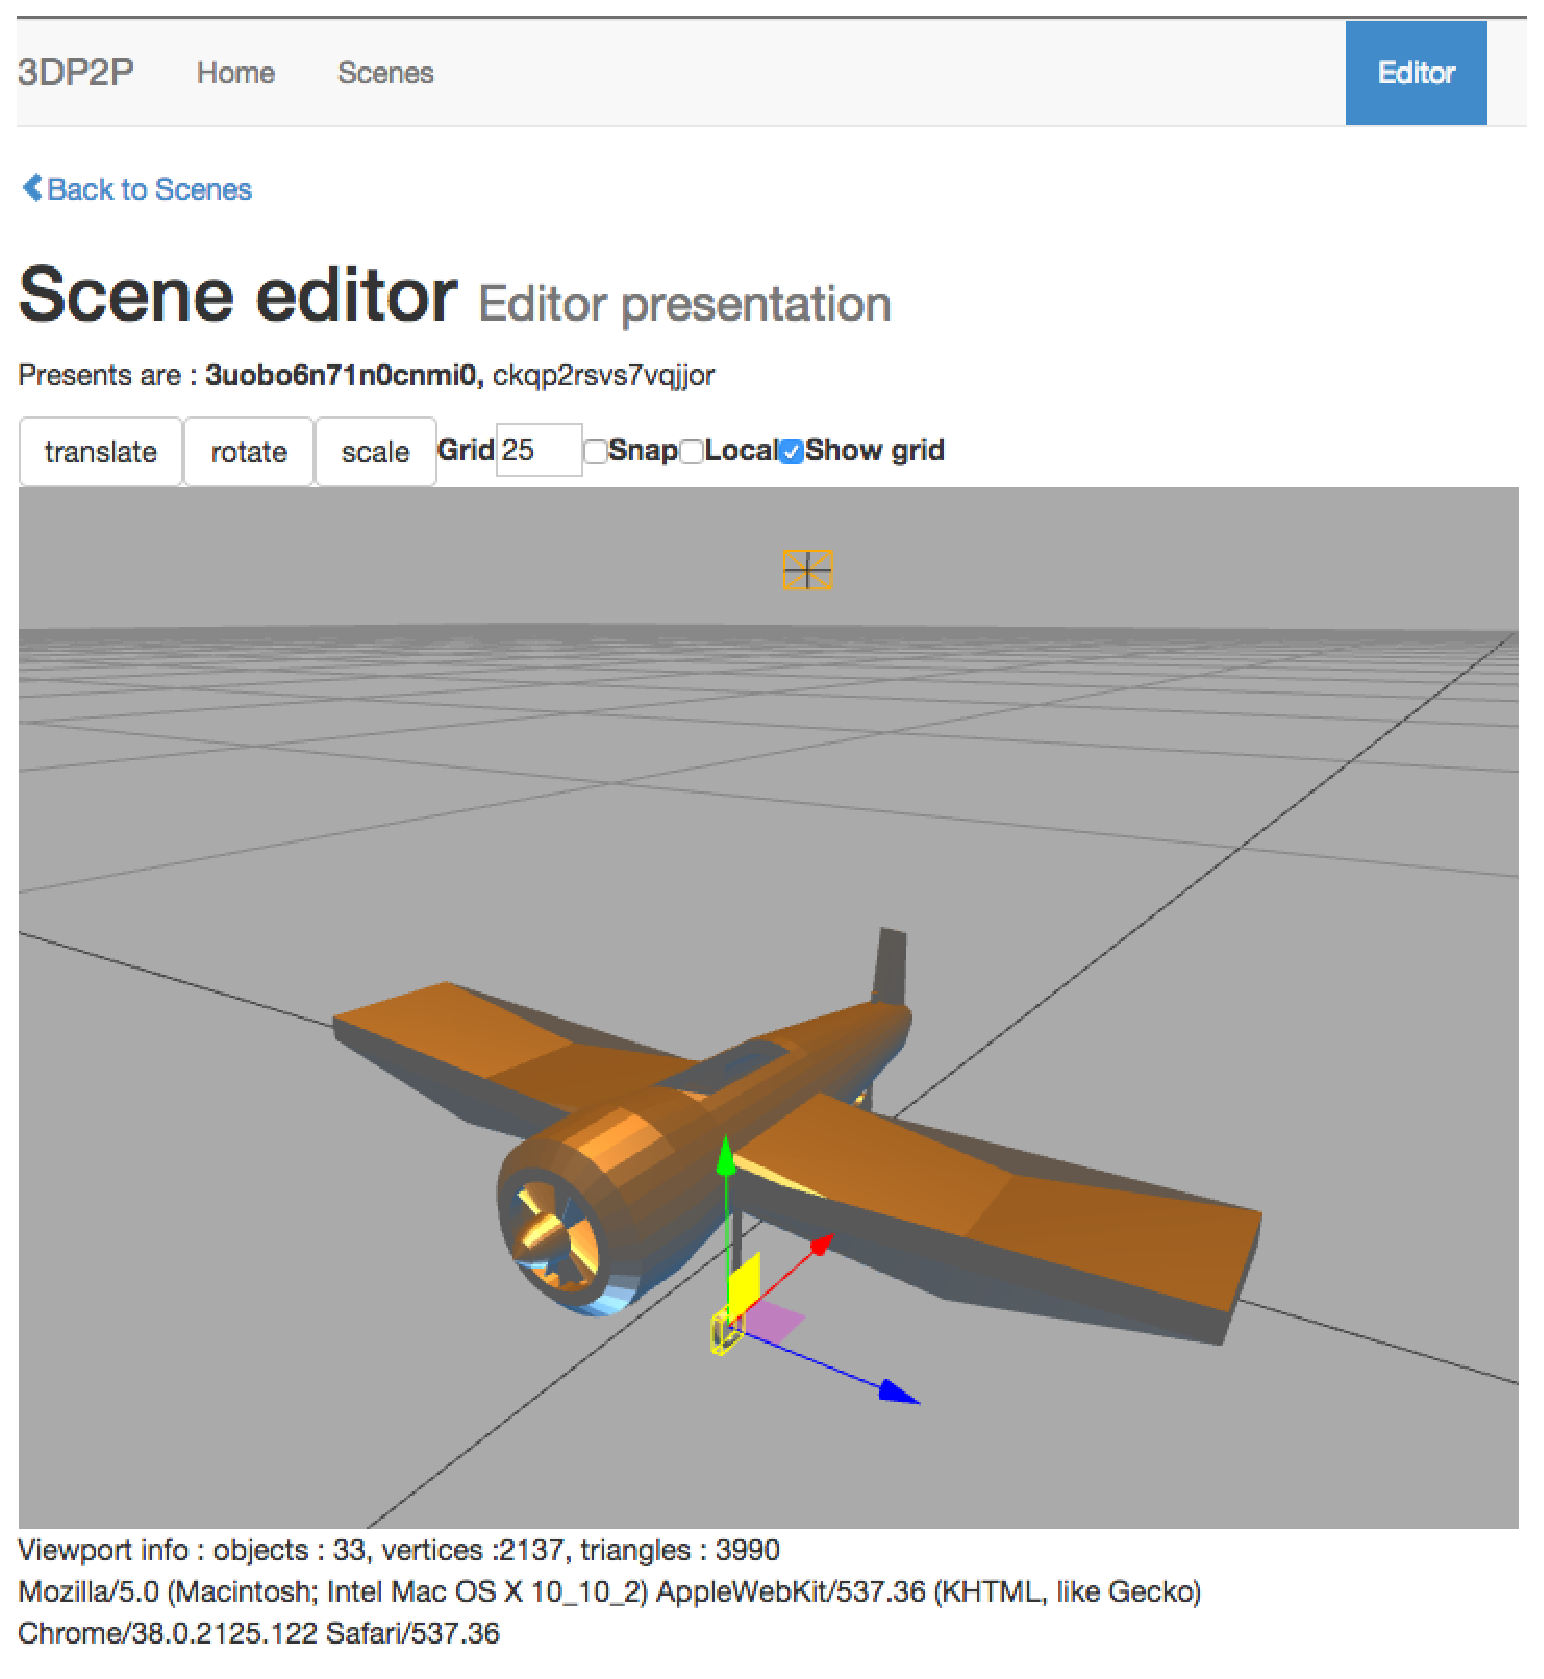
\includegraphics[width=0.6\columnwidth]{eps/editorpresentation.eps}
	\caption{Interface de 3DState}
	\label{fig:3Dstateinterface}
\end{figure}

\subsection{Gestion de la session}
Lorsqu'un utilisateur rejoint une session, il suit le déroulement des opérations 
décrit dans la Figure \ref{fig:sequence_state}. 
Dans un premier temps, afin de récupérer les données liées à l'espace de travail, 
le client web de l'utilisateur qui se rend sur une scène récupère 
tous les objets associés à la scène dans la base de données. Les objets de la 
scène sont renvoyés à l'éditeur pour les afficher. 
Dans un second temps, le système établit les connexions \gls{P2P} entre les 
clients de manière automatique et complète (topologie réseau en maillage 
complet) après avoir récupéré les identifiants des autres utilisateurs auprès du 
serveur de \textit{signaling}. Une fois la connexion établie, chaque collaborateur 
voit son environnement \gls{3D} dans l'éditeur mis à jour, indiquant la position du 
nouvel 
arrivant. Les collaborateurs éditent ensuite la scène \gls{3D} qui produit, sur les 
différents objets, des requêtes \gls{CRUD} -- incluant les opérations de translation, 
rotation et homothétie -- destinées au serveur (qui transmet les 
modifications à la base de données) puis aux collaborateurs.
Enfin, dans un dernier temps, lorsque l'utilisateur quitte la scène, il en notifie le 
serveur de \textit{signaling} qui s'occupe d'indiquer aux clients restants l'abandon 
du client pour qu'ils puissent mettre à jour leur interface en conséquence.

\begin{figure}[ht!]
	\centering
	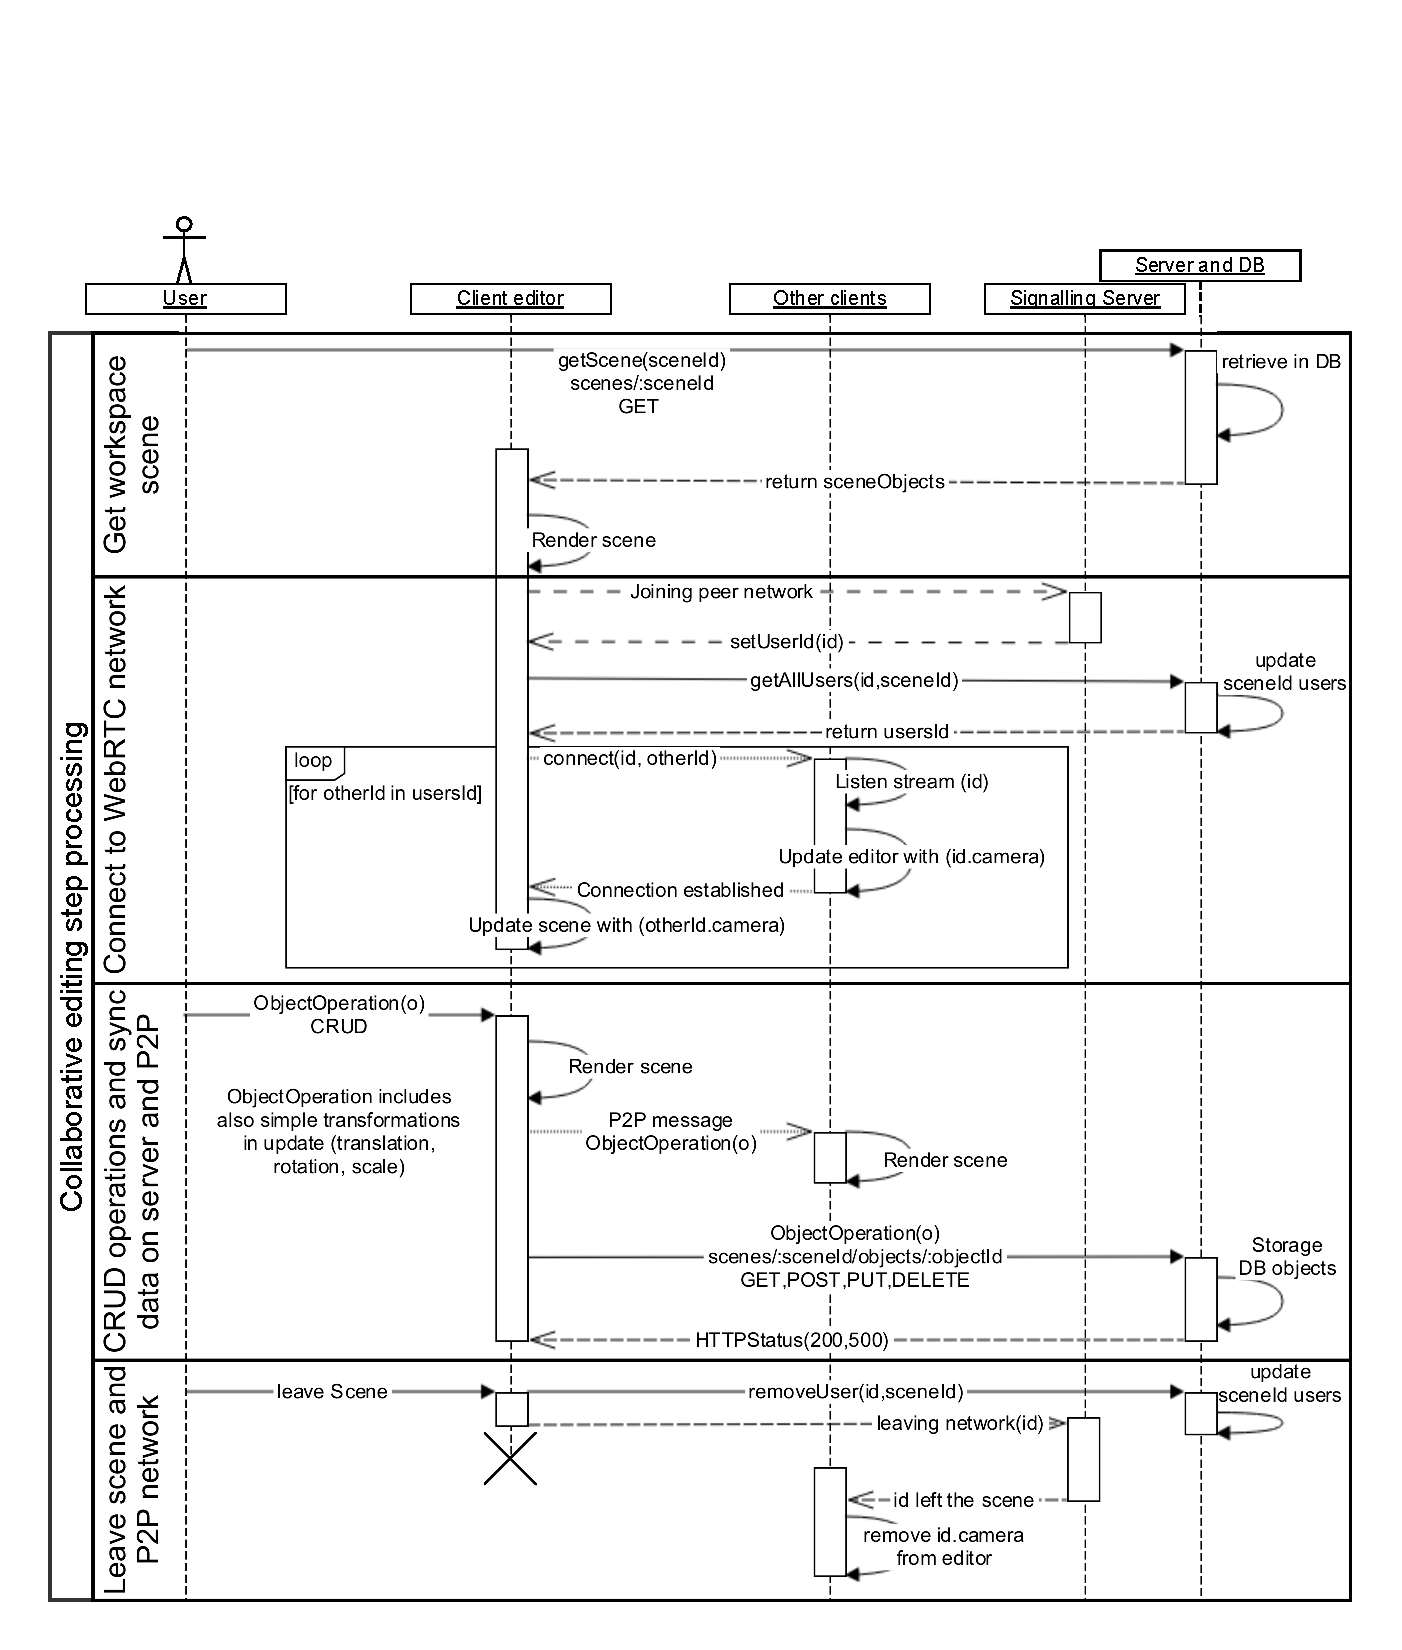
\includegraphics[trim={0 0 0 3cm},clip,width=1\columnwidth]
	{eps/sequence_wscg.eps}
	\caption{Diagramme de séquence de la gestion de la session dans une 
		architecture \og orientée état\fg{}}
	\label{fig:sequence_state}
\end{figure}

		
		\subsection{Bilan critique}
		
		
			\paragraph{Résumé des choix techniques}
			
			\begin{table}[!h]
				\centering
\caption{\label{table:3DStateChoixTechniques}Résumé des choix techniques pour 
3DState}
\begin{tabular}{llll}
	& \textbf{Plateforme / Service}& \textbf{Bibliothèque (version)}\\ \hline
	& \begin{tabular}[c]{@{}l@{}}
		Rendu WebGL \\ 
		Gestionnaire d'événements 
	\end{tabular} 	& 
	\begin{tabular}[c]{@{}l@{}}
		Three.JS (r69) \\ 
		signal-js (v1.0.0)
	\end{tabular}\\
	\multirow{-3}{*}{\textbf{Pair}} & WebRTC & PeerJS (v0.3.9)\\ \hline
	& Node.JS (v0.10.32)& ExpressJS (v4.9.0)\\
	& WebSocket & PeerJSServer (N/A) \\
	\multirow{-3}{*}{\textbf{Serveur}} & Base de données NoSQL & MongoDB 
	(v2.6.8) \\ \hline
\end{tabular}
\end{table}
			
			\paragraph{Testabilité}

\section{3DEvent : une approche découplée orientée événements}
\subsection{Intergiciel pour l'échange de 3D par événements}
\subsubsection{Données d'échanges}
\subsubsection{Synchronisation des données}
\subsubsection{Gestion de la cohérence}

\subsection{Interface orientée tâche}
Dans le but de proposer une \gls{IU} proche des fonctionnalités métiers liées à la 
modélisation \gls{3D}, l'éditeur possède une interface orientée \og tâche\fg{}, en 
comparaison avec des \gls{IU} \gls{CRUD}. En effet, les \gls{IU} \gls{CRUD} 
réduisent la sémantique métier du domaine d'application à la création, la lecture, la 
mise à jour et la suppression, omettant toutes les subtilités que peuvent dégager 
ces actions en perdant l'intention de l'utilisateur dès le niveau de l'interface. Une 
interface orientée tâche a tendance à s'attarder sur toutes les nuances que le 
domaine possède en caractérisant chaque action sans subir d'effet de 
simplification. Cette proximité avec le métier permet de calquer directement 
l'interface du modèle événementiel sur l'\gls{IU} et de guider l'utilisateur dans ses 
activités. L'utilisabilité, qualité de l'expérience utilisateur fournit par un système 
pour réaliser une tâche, est alors maximisée en terme d'efficacité, d'efficience et 
de satisfaction. 
Ce type d'\gls{IHM} s'organise autour de cas d'utilisation. Cela permet, 
d'une part, de présenter clairement les 
actions (\og ajouter une géométrie à la 
bibliothèque à partir d'un fichier\fg{} plutôt que \og téléverser un fichier\fg{}) : 
l'intention est clairement définie. D'autre part, lorsque l'utilisateur s'apprête à faire 
une action, seules les informations utiles sont affichées. Enfin, l'application fournit 
simplement l'information dans le contexte où elle doit être présentée, évitant à 
l'utilisateur d'aller la chercher ailleurs.
L'\gls{IU} devient alors une couche de l'application qui nécessite d'agréger, croiser 
et filtrer des données. La dénormalisation proposée par \gls{CQRS} remédie à ce 
besoin dans le cadre de la consultation de données. 


\subsubsection{Présentation de l'interface}


%\begin{figure}[h!]
%	\centering
%	\begingroup
%	
%	\subfloat[Rotation (vue \gls{3D}) et outils de manipulation d'objet 
%	\gls{3D} 
%	(panneau 
%	
%latéral)]{\includegraphics[width=0.75\textwidth]{eps/2rotatedetail.eps}\label{fig:ui2}}\hfill
%	
%	\subfloat[Translation (vue \gls{3D}) et visualisation de l'historique 
%	(panneau 
%	
%latéral)]{\includegraphics[width=0.75\textwidth]{eps/1translatehisto.eps}\label{fig:ui1}}\hfill
%	
%	\subfloat[Mise à l'échelle (vue \gls{3D}) et liste des collaborateurs 
%	(panneau 
%	
%latéral)]{\includegraphics[width=0.75\textwidth]{eps/3scalecollab.eps}\label{fig:ui3}}\hfill
%	
%	\endgroup
%	\caption{Interface utilisateur pendant une session collaborative (trois 
%personnes)}
%	\label{fig:screenshots}
%\end{figure}
Lorsqu'un utilisateur se connecte à une scène, il a accès à une interface web 
(dans un navigateur) qui représente l'espace de travail collaboratif et qui lui 
permettant 
d'utiliser différentes fonctionnalités. Les deux modalités d'interaction sont le clavier 
et la souris\info{est ce qu'on parle de mobile?}. Le premier niveau de cette 
interface est scindée en deux panneaux~: 
\begin{enumerate}
	\item L'espace \gls{3D} consacré à la visualisation des objets et à leur 
	manipulation 
	dans l'environnement \gls{3D}~;
	\item La barre d'outils qui contient trois onglets~:~
	\begin{enumerate}
		\item "Scene" contient tous les détails de la scène et des maillages qu'elle 
		inclue~; 
		\item "Collaboration" fournit les informations liées à la collaboration~;
		\item "History" liste tous les événements qui ont eut lieu dans la scène et 
		leurs  détails. 
	\end{enumerate}
\end{enumerate}

\begin{figure}[ht]
	\centering
	\begingroup
	
	\subfloat[Onglet \og outils de manipulation sur la 
	scène\fg{}]{\includegraphics[width=0.38\textwidth]{eps/scenecontrol.eps}\label{fig:uicontrol}}
	\hfill
	\subfloat[Onglet \og collaboration\fg{}]
	{\includegraphics[width=0.27\textwidth]{eps/collaboration.eps}\label{fig:uicollab}} 
	\hfill
	\subfloat[Onglet \og 
	historique\fg{}]{\includegraphics[width=0.32\textwidth]{eps/history.eps}\label{fig:uihisotry}}
	
	\endgroup
	\caption{Onglets du panneau latéral de l'interface}
	\label{fig:uipanneau}
\end{figure}
La Figure \ref{fig:uipanneau} montre quelques captures d'écran durant une 
session collaborative sur le modèle Rotor.

L'onglet "Scene" (Figure \ref{fig:uicontrol}) possède un bloc contenant les détails 
d'un 
maillage en cours de 
sélection. Cela permet d'avoir la description des propriétés de l'objet sélectionné et 
une manipulation de ses paramètres (position, rotation et mise à l'échelle) plus 
précise que via l'espace \gls{3D} avec le cliqué / déplacé. "Scene" intègre 
également un espace réservé aux géométries disponibles dans la scène appelé 
Bibliothèque (de géométries).

L'onglet "Collaboration" (Figure \ref{fig:uicollab}) présente la liste des 
collaborateurs qui 
participent à la 
scène. Chacun d'eux est décrit par son nom, son état  (connecté ou déconnecté) 
et son rôle (administrateur, éditeur, lecteur ou autre\footnote{Un rôle peut être 
	défini par le biais du \gls{framework} 3DEvent}). En cliquant sur un élément de 
	la 
liste, l'utilisateur accède au dernier point de vue dans l'espace \gls{3D} connu du 
collaborateur représenté.

L'onglet "History" (Figure \ref{fig:uihisotry}) liste tous les événements passés dans 
la 
scène en fournissant 
l'accès à leur détail. Pour chaque événement, le système est capable de montrer 
dans l'espace \gls{3D} la différence entre l'état  après l'événement cliqué $state_x$ 
et l'état courant $state_n$. L'utilisateur peut à partir de cette visualisation choisir 
de \og revenir en arrière\fg{} sans perdre les données entre $state_n$ et $state_x$ 
car dans le système présenté ici, cela s'effectue par compensation (cf 
Event-Sourcing 
Section X)\improve{annulation d'un événement ou juste ES}.

Dans chaque onglet se trouvent différents blocs \gls{HTML}, avec des 
comportements spécifiques à un agrégat et injectés dynamiquement. Ces blocs 
correspondent aux views de ce modèle.

Les boîtes englobantes représentent la sélection des différents collaborateurs 
pendant la session.

Parmi les views disponibles dans le système, une grande partie est dédiée à 
l'\gls{IU} de l'application web pour le cas d'utilisation de la modélisation 3D. 
D'autres views sont disponibles pour un autre type d'utilisation destinée à 
l'observation des comportements des utilisateurs, élément est primordiale dans 
une expérimentations.



\paragraph{Exemple d'interaction}
La Figure \ref{fig:cqrs-example} décrit la façon dont le système traite l'exécution 
d'une commande de translation déclenchée par l'utilisateur et comment cette 
information est diffusée aux collaborateurs\footnote{Pour que l'exemple 
	fonctionne, la scène, la géométrie du cube et le maillage \textit{cube1} doivent 
	avoir été créés en amont.}.
Dans l'étape (a), la commande déclenchée par l'utilisateur s'adresse à l'agrégat 
$cube1$ et contient les paramètres de la translation (vecteur x, y, z). L'agrégat, 
qui 
modélise le domaine d'un maillage, génère l'événement de translation $e1$ (étape 
(b)) si tout est valide d'un point de vue métier. L'événement $e1$ est ensuite 
passé à l'Event Store. 
Le composant responsable de la détection de conflit permet au développeur 
d'implémenter ses propres règles de résolution de conflit. Le composant déclenche 
une exception lorsque le numéro de version reçu et le numéro de version courant 
de l'agrégat sont identiques (Figure \ref{fig:cqrs-example} étape (c)). Selon les 
règles métiers définies et les exceptions liées à la cohérence, l'événement peut 
être 
rejeté. Ce traitement peut être à l'origine de la génération de nouveaux 
événements.


\begin{figure}[]
	\centering
	\includegraphics[width=\columnwidth]{eps/example10.eps}
	\caption[Flux de la collaboration dans le framework 3DEvent entre 3 
	utilisateurs]{Exemple d'édition collaborative où User A est connecté à User  B, 
		lui 
		même connecté à User C. Le cycle montre les différentes étapes du 
		déclenchement: la commande, la 
		génération 
		de l'événement, la 
		synchronisation du journal d'événements, l'impact sur le rendu des autres 
		utilisateurs pour une translation sur un cube et le rendu 
		visuel.}\label{fig:cqrs-example}
\end{figure}

\subsection{Sélection fantôme}
Les interactions utilisateurs doivent être adaptées à la collaboration et aux 
manipulations à effectuer. Pour cela, l'éditeur 3DEvent introduit la fonctionnalité de 
sélection \og fantôme\fg{}. Lorsqu'un utilisateur souhaite sélectionner un objet de 
la scène, l'objet original ($O_o$) est 
cloné et devient l'objet fantôme ($O_f$). $O_f$ conservent les mêmes propriétés, 
représenté avec de la 
transparence d'où le terme \og fantôme\fg{}. 
L'objet $O_f$ prend alors le focus de sélection pour que l'utilisateur le manipule à 
la place de l'objet $O_f$. 
Lorsque l'utilisateur relâche $O_f$, alors la modification intentée s'applique sur 
$O_o$ avec le principe du \textit{Last Write Wins} (le dernier gagne).
La Figure \ref{fig:ghostselection} 
représente la sélection fantôme lors de la translation du corps du rotor par 
l'utilisateur Foo : c'est l'objet transparent qui est manipulé alors que l'objet opaque 
représente sa position originale. 
En différenciant l'actuel objet que l'utilisateur souhaite sélectionné ($O_{o}$) de 
celui manipulé ($O_f$), l'interaction est mise en valeur sous quatre angles :
\begin{itemize}
	\item l'ergonomie dans l'environnement \gls{3D} :
	$O_f$ est un objet temporaire qui permet à l'utilisateur
	d'avoir une visualisation de l'objet en cours de manipulation tout en 
	conservant le dernier état de $O_o$ visible. 
	$O_o$ peut être considéré comme un point de repère visuel pour l'utilisateur 
	lorsqu'il effectue sa manipulation. 
	L'$O_f$ a aussi un rôle d'intermédiaire entre l'utilisateur et la 
	finalité de l'interaction en donnant un support visuel à sa réflexion experte.
	Grâce à $O_f$, l'utilisateur peut également révoquer sa manipulation en 
	cours sans avoir eu d'impact sur $O_o$ en évitant des actions inutiles (faire 
	l'action 
	puis la défaire) pour le métier et coûteuses pour le réseau.
	
	\item la collaboration : si un collaborateur effectue une modification 
	à destination du même $O_o$ alors la représentation de $O_o$ chez 
	l'utilisateur est également modifiée. $O_f$ par contre ne subit pas d'impact ; 
	l'utilisateur peut continuer sa manipulation et~/~ou l'ajuster en fonction des 
	nouvelles informations liées à $O_o$ ou même révoquer sa manipulation 
	en cours si cela lui convient.
	
	\item le métier : seules les manipulations menées à terme sont 
	considérées comme des commandes. Cela évite d'avoir des événements qui ne 
	sont pas pertinents pour le métier dans le journal d'événements (comme lorsque 
	l'utilisateur change d'idée lors de l'interaction ou
	suite à une intervention concurrente). L'utilisateur n'a un impact sur l'application 
	que lorsqu'une modification métier est réalisée.
	
	\item le réseau : l'information importante à faire transité est l'événement 
	correspondant à la modification métier pas toutes les positions intermédiaires 
	même si intuitivement l'idée de temps réel pourrait conduire à cette solution. La 
	quantité de messages produite surchargerai à la fois le réseau et le fil 
	d'exécution principale de l'application. En effet, \gls{WebRTC} a l'inconvénient 
	pour le 
	moment de ne pas pouvoir s'exécuter dans un \textit{Web Worker} (fil 
	d'exécution 
	parallèle en JavaScript). Cette solution imposerai des 
	latences réseau et d'\gls{IU} qui affecteraient gravement l'expérience utilisateur
	sans apporter d'informations supplémentaires à l'aspect métier de la 
	collaboration. 
\end{itemize}


\begin{figure}[ht]
	\centering
	\includegraphics[trim={0 0 0cm 0}, clip, 
	width=0.8\columnwidth]{eps/1translatehisto.eps}
	\caption{Illustration de la sélection fantôme dans l'environnement 3D}
	\label{fig:ghostselection}
\end{figure}


\subsection{Bilan}
\paragraph{Testabilité}

% ----- chapitre Expérimentations et résultats
%!TEX root = main.tex
\chapter{Expérimentations}
\chaptertable
\section{Cas d'étude : Assemblage collaboratif d'objets 3D dans un 
environnement web}
Dans \cite{Desprat2015a} et \cite{Desprat2017}, 


\section{Expérimentation 1 : preuve de faisabilité}
Cette expérimentation est tirée de l'article \cite{Desprat2015a}.
Un des objectifs de cette expérimentation est de démontrer la faisabilité de notre 
approche réseau hybride avec une attention particulière à l'égard de l'expérience 
utilisateur.
\subsection{Présentation de l'expérimentation}

\subsection{Résultats}
\subsection{Discussion et Conclusion}

\section{Expérimentation 2 : Intégration du framework évènementiel}
\label{sec:us}
\input{51_xp_debs2017}





\section{Comparaison entre l'expérimentation 1 et l'expériementation 2}
\subsection{Résultats}
\subsection{Discussion et Conclusion}


% ----- chapitre Conclusion
%!TEX root = main.tex
\chapter{Conclusion}
\chaptertable

% ----- chapitre Annexes
\begin{appendix}
	\chapter{Description des évènements}
	\begin{landscape}
\begin{table}[]
	
	\centering
	\caption{3DEvent : résumé des évènements par agrégats}
	\label{tab:events}
	\begin{tabular}{lll}
		\toprule
		\textbf{Évènement}& \textbf{Nommage} & \textbf{Description} \\ \midrule
		\textbf{Agrégat Scène}     &                      &             \\ \hline
		Scène créée &  sceneCreated                  & Une scène a été 
		créée            \\
		Scène supprimée &        sceneRemoved              &  Une scène a été 
		supprimée           \\
		Scène renommée &     sceneRenamed                 &     Une scène a été 
		renommée        \\
		\textbf{Agrégat Maillage}  &                      &             \\ \hline
		Maillage ajouté &     meshAdded                 
		&  \begin{tabular}[c]{@{}l@{}} Un maillage a été ajouté dans la Scène à 
		partir \\d'une géométrie de la 
		bibliothèque \end{tabular}  \\
		Maillage déposé &     meshDropped               
		&      \begin{tabular}[c]{@{}l@{}} Un maillage a été déposé dans 
		l'environnement 3D\\ de la Scène à 
		partir d'une géométrie de la bibliothèque \end{tabular} \\
		Maillage supprimé & meshRemoved       &           Un maillage a été 
		supprimé de la Scène   \\
		Maillage translaté &   meshTranslated  	 &    Un maillage a 
		subit une translation dans la Scène         \\
		Maillage pivoté &      meshRotated                &     Un maillage a 
		subit une rotation dans la Scène              \\
		Maillage mis à l'échelle &  meshScaled           &      Un maillage a 
		subit une homothétie dans la Scène         \\
		\textbf{Agrégat Géométrie} &                      &             \\ \hline
		Géométrie importé dans la bibliothèque &  geometryImported           &        
		\begin{tabular}[c]{@{}l@{}} Une géométrie est créée à partir d'un fichier 
		importé par\\ 
		un utilisateur et ajoutée à la bibliothèque de la 
		Scène \end{tabular}     \\
		\textbf{Agrégat Utilisateur}        &                      &            \\ \hline
		Utilisateur créé&   userCreated                   &        Un utilisateur a été créé 
		dans l'application    \\
		Scène rejointe par utilisateur&     userJoinedScene                 &      Un 
		utilisateur a rejoint une scène       \\
		Scène quittée par utilisateur&        userLeftScene              &    Un utilisateur 
		a quitté une scène         \\
		Nom modifié &         usernameChanged           &     Un utilisateur a modifié 
		son nom        \\
		Couleur modifiée &       colorChanged                  &      Un utilisateur a 
		modifié son code couleur       \\ \bottomrule
	\end{tabular}
\end{table}

\end{landscape}

\chapter{Messages réseaux pour la synchronisation des Event Stores}

\begin{table}[]
	\centering
	\small
	\caption{Type de messages lors de la synchronisation}
	\label{table:messagetype}
	\begin{tabular}{ll}
		\toprule
		\textbf{Message}                & \textbf{Description} \\ \hline
		STREAM\_SYNC\_ASK      &  Demande de synchronisation d'un 
		\textit{stream}           \\
		CHUNK                  &     Réception d'une donnée \textit{chunk})        
		\\
		READY\_ASK             &      Prêt pour la démarrer la demande de 
		données de 
		sync.        \\
		READY                  &       Prêt pour démarrer la réception de 
		données de 
		sync.      \\
		ALL\_EVENTS\_SYNC\_ASK &     Demande de toutes les données 
		typées 
		évènement           \\
		EVENTS\_SYNC           &        Réception de données (en cours de 
		synchronisation)       \\
		META\_DATA\_ASK        &     Demande de métadonnées       \\
		META\_DATA             &      Réception de métadonnées       \\
		SYNC                   &      Réception de données (en cours de 
		synchronisation)         \\
		EVENT                  &     Réception d'une donnée typée 
		évènement        \\
		END\_SYNC              & Fin de la synchronisation \\ \bottomrule
	\end{tabular}
\end{table}
\todo{parler des tableaux}

\begin{table}[]
	\centering
	\caption{Statut du n\oe ud}
	\label{table:nodestatus}
	\begin{tabular}{ll}
		\toprule
		\textbf{Message}             & \textbf{Description} \\ \midrule
		ERROR               &      En erreur (désynchronisation)       \\
		READY               &       Prêt à recevoir des messages      \\
		META\_DATA\_ASK     &      En demande de métadonnées       \\
		META\_DATA\_RECEIVE &      En réception de métadonnées       \\
		CLOSE               &     Déconnecté (connexion fermée)        \\
		RECEIVE\_SYNC       &      En réception de données à synchroniser    \\
		CONNECTED           &      Connecté (connexion ouverte)        \\
		INIT                &     Initialisation   \\
		OK                  &    Connecté et synchronisé      \\
		SEND\_SYNC          &    En demande de synchronisation         \\
		END\_SYNC           &      Synchronisation terminée      \\ \bottomrule
	\end{tabular}
\end{table}
\end{appendix}

\backmatter

\completelist
\singlespacing
\bibliographystyle{apalike-fr}
%	\bibliography{references}
\bibliography{mendeley}
\end{document}